% Options for packages loaded elsewhere
\PassOptionsToPackage{unicode}{hyperref}
\PassOptionsToPackage{hyphens}{url}
\PassOptionsToPackage{dvipsnames,svgnames,x11names}{xcolor}
%
\documentclass[
  12pt,
  letterpaper,
  DIV=11,
  numbers=noendperiod]{scrreport}

\usepackage{amsmath,amssymb}
\usepackage{iftex}
\ifPDFTeX
  \usepackage[T1]{fontenc}
  \usepackage[utf8]{inputenc}
  \usepackage{textcomp} % provide euro and other symbols
\else % if luatex or xetex
  \usepackage{unicode-math}
  \defaultfontfeatures{Scale=MatchLowercase}
  \defaultfontfeatures[\rmfamily]{Ligatures=TeX,Scale=1}
\fi
\usepackage{lmodern}
\ifPDFTeX\else  
    % xetex/luatex font selection
\fi
% Use upquote if available, for straight quotes in verbatim environments
\IfFileExists{upquote.sty}{\usepackage{upquote}}{}
\IfFileExists{microtype.sty}{% use microtype if available
  \usepackage[]{microtype}
  \UseMicrotypeSet[protrusion]{basicmath} % disable protrusion for tt fonts
}{}
\makeatletter
\@ifundefined{KOMAClassName}{% if non-KOMA class
  \IfFileExists{parskip.sty}{%
    \usepackage{parskip}
  }{% else
    \setlength{\parindent}{0pt}
    \setlength{\parskip}{6pt plus 2pt minus 1pt}}
}{% if KOMA class
  \KOMAoptions{parskip=half}}
\makeatother
\usepackage{xcolor}
\usepackage[lmargin=1.2in,rmargin=1.2in,tmargin=1.2in,bmargin=1.2in]{geometry}
\setlength{\emergencystretch}{3em} % prevent overfull lines
\setcounter{secnumdepth}{5}
% Make \paragraph and \subparagraph free-standing
\ifx\paragraph\undefined\else
  \let\oldparagraph\paragraph
  \renewcommand{\paragraph}[1]{\oldparagraph{#1}\mbox{}}
\fi
\ifx\subparagraph\undefined\else
  \let\oldsubparagraph\subparagraph
  \renewcommand{\subparagraph}[1]{\oldsubparagraph{#1}\mbox{}}
\fi

\usepackage{color}
\usepackage{fancyvrb}
\newcommand{\VerbBar}{|}
\newcommand{\VERB}{\Verb[commandchars=\\\{\}]}
\DefineVerbatimEnvironment{Highlighting}{Verbatim}{commandchars=\\\{\}}
% Add ',fontsize=\small' for more characters per line
\usepackage{framed}
\definecolor{shadecolor}{RGB}{241,243,245}
\newenvironment{Shaded}{\begin{snugshade}}{\end{snugshade}}
\newcommand{\AlertTok}[1]{\textcolor[rgb]{0.68,0.00,0.00}{#1}}
\newcommand{\AnnotationTok}[1]{\textcolor[rgb]{0.37,0.37,0.37}{#1}}
\newcommand{\AttributeTok}[1]{\textcolor[rgb]{0.40,0.45,0.13}{#1}}
\newcommand{\BaseNTok}[1]{\textcolor[rgb]{0.68,0.00,0.00}{#1}}
\newcommand{\BuiltInTok}[1]{\textcolor[rgb]{0.00,0.23,0.31}{#1}}
\newcommand{\CharTok}[1]{\textcolor[rgb]{0.13,0.47,0.30}{#1}}
\newcommand{\CommentTok}[1]{\textcolor[rgb]{0.37,0.37,0.37}{#1}}
\newcommand{\CommentVarTok}[1]{\textcolor[rgb]{0.37,0.37,0.37}{\textit{#1}}}
\newcommand{\ConstantTok}[1]{\textcolor[rgb]{0.56,0.35,0.01}{#1}}
\newcommand{\ControlFlowTok}[1]{\textcolor[rgb]{0.00,0.23,0.31}{#1}}
\newcommand{\DataTypeTok}[1]{\textcolor[rgb]{0.68,0.00,0.00}{#1}}
\newcommand{\DecValTok}[1]{\textcolor[rgb]{0.68,0.00,0.00}{#1}}
\newcommand{\DocumentationTok}[1]{\textcolor[rgb]{0.37,0.37,0.37}{\textit{#1}}}
\newcommand{\ErrorTok}[1]{\textcolor[rgb]{0.68,0.00,0.00}{#1}}
\newcommand{\ExtensionTok}[1]{\textcolor[rgb]{0.00,0.23,0.31}{#1}}
\newcommand{\FloatTok}[1]{\textcolor[rgb]{0.68,0.00,0.00}{#1}}
\newcommand{\FunctionTok}[1]{\textcolor[rgb]{0.28,0.35,0.67}{#1}}
\newcommand{\ImportTok}[1]{\textcolor[rgb]{0.00,0.46,0.62}{#1}}
\newcommand{\InformationTok}[1]{\textcolor[rgb]{0.37,0.37,0.37}{#1}}
\newcommand{\KeywordTok}[1]{\textcolor[rgb]{0.00,0.23,0.31}{#1}}
\newcommand{\NormalTok}[1]{\textcolor[rgb]{0.00,0.23,0.31}{#1}}
\newcommand{\OperatorTok}[1]{\textcolor[rgb]{0.37,0.37,0.37}{#1}}
\newcommand{\OtherTok}[1]{\textcolor[rgb]{0.00,0.23,0.31}{#1}}
\newcommand{\PreprocessorTok}[1]{\textcolor[rgb]{0.68,0.00,0.00}{#1}}
\newcommand{\RegionMarkerTok}[1]{\textcolor[rgb]{0.00,0.23,0.31}{#1}}
\newcommand{\SpecialCharTok}[1]{\textcolor[rgb]{0.37,0.37,0.37}{#1}}
\newcommand{\SpecialStringTok}[1]{\textcolor[rgb]{0.13,0.47,0.30}{#1}}
\newcommand{\StringTok}[1]{\textcolor[rgb]{0.13,0.47,0.30}{#1}}
\newcommand{\VariableTok}[1]{\textcolor[rgb]{0.07,0.07,0.07}{#1}}
\newcommand{\VerbatimStringTok}[1]{\textcolor[rgb]{0.13,0.47,0.30}{#1}}
\newcommand{\WarningTok}[1]{\textcolor[rgb]{0.37,0.37,0.37}{\textit{#1}}}

\providecommand{\tightlist}{%
  \setlength{\itemsep}{0pt}\setlength{\parskip}{0pt}}\usepackage{longtable,booktabs,array}
\usepackage{multirow}
\usepackage{calc} % for calculating minipage widths
% Correct order of tables after \paragraph or \subparagraph
\usepackage{etoolbox}
\makeatletter
\patchcmd\longtable{\par}{\if@noskipsec\mbox{}\fi\par}{}{}
\makeatother
% Allow footnotes in longtable head/foot
\IfFileExists{footnotehyper.sty}{\usepackage{footnotehyper}}{\usepackage{footnote}}
\makesavenoteenv{longtable}
\usepackage{graphicx}
\makeatletter
\def\maxwidth{\ifdim\Gin@nat@width>\linewidth\linewidth\else\Gin@nat@width\fi}
\def\maxheight{\ifdim\Gin@nat@height>\textheight\textheight\else\Gin@nat@height\fi}
\makeatother
% Scale images if necessary, so that they will not overflow the page
% margins by default, and it is still possible to overwrite the defaults
% using explicit options in \includegraphics[width, height, ...]{}
\setkeys{Gin}{width=\maxwidth,height=\maxheight,keepaspectratio}
% Set default figure placement to htbp
\makeatletter
\def\fps@figure{htbp}
\makeatother
\newlength{\cslhangindent}
\setlength{\cslhangindent}{1.5em}
\newlength{\csllabelwidth}
\setlength{\csllabelwidth}{3em}
\newlength{\cslentryspacingunit} % times entry-spacing
\setlength{\cslentryspacingunit}{\parskip}
\newenvironment{CSLReferences}[2] % #1 hanging-ident, #2 entry spacing
 {% don't indent paragraphs
  \setlength{\parindent}{0pt}
  % turn on hanging indent if param 1 is 1
  \ifodd #1
  \let\oldpar\par
  \def\par{\hangindent=\cslhangindent\oldpar}
  \fi
  % set entry spacing
  \setlength{\parskip}{#2\cslentryspacingunit}
 }%
 {}
\usepackage{calc}
\newcommand{\CSLBlock}[1]{#1\hfill\break}
\newcommand{\CSLLeftMargin}[1]{\parbox[t]{\csllabelwidth}{#1}}
\newcommand{\CSLRightInline}[1]{\parbox[t]{\linewidth - \csllabelwidth}{#1}\break}
\newcommand{\CSLIndent}[1]{\hspace{\cslhangindent}#1}

\KOMAoption{captions}{tableheading}
\makeatletter
\makeatother
\makeatletter
\@ifpackageloaded{bookmark}{}{\usepackage{bookmark}}
\makeatother
\makeatletter
\@ifpackageloaded{caption}{}{\usepackage{caption}}
\AtBeginDocument{%
\ifdefined\contentsname
  \renewcommand*\contentsname{Tabla de contenidos}
\else
  \newcommand\contentsname{Tabla de contenidos}
\fi
\ifdefined\listfigurename
  \renewcommand*\listfigurename{Listado de Figuras}
\else
  \newcommand\listfigurename{Listado de Figuras}
\fi
\ifdefined\listtablename
  \renewcommand*\listtablename{Listado de Tablas}
\else
  \newcommand\listtablename{Listado de Tablas}
\fi
\ifdefined\figurename
  \renewcommand*\figurename{Figura}
\else
  \newcommand\figurename{Figura}
\fi
\ifdefined\tablename
  \renewcommand*\tablename{Tabla}
\else
  \newcommand\tablename{Tabla}
\fi
}
\@ifpackageloaded{float}{}{\usepackage{float}}
\floatstyle{ruled}
\@ifundefined{c@chapter}{\newfloat{codelisting}{h}{lop}}{\newfloat{codelisting}{h}{lop}[chapter]}
\floatname{codelisting}{Listado}
\newcommand*\listoflistings{\listof{codelisting}{Listado de Listados}}
\makeatother
\makeatletter
\@ifpackageloaded{caption}{}{\usepackage{caption}}
\@ifpackageloaded{subcaption}{}{\usepackage{subcaption}}
\makeatother
\makeatletter
\@ifpackageloaded{tcolorbox}{}{\usepackage[skins,breakable]{tcolorbox}}
\makeatother
\makeatletter
\@ifundefined{shadecolor}{\definecolor{shadecolor}{rgb}{.97, .97, .97}}
\makeatother
\makeatletter
\makeatother
\makeatletter
\makeatother
\ifLuaTeX
\usepackage[bidi=basic]{babel}
\else
\usepackage[bidi=default]{babel}
\fi
\babelprovide[main,import]{spanish}
% get rid of language-specific shorthands (see #6817):
\let\LanguageShortHands\languageshorthands
\def\languageshorthands#1{}
\ifLuaTeX
  \usepackage{selnolig}  % disable illegal ligatures
\fi
\IfFileExists{bookmark.sty}{\usepackage{bookmark}}{\usepackage{hyperref}}
\IfFileExists{xurl.sty}{\usepackage{xurl}}{} % add URL line breaks if available
\urlstyle{same} % disable monospaced font for URLs
\hypersetup{
  pdftitle={Reloj inteligente IoT basado en tecnologías abiertas para la recopilación de datos de confort térmico},
  pdfauthor={Julio César Landa López},
  pdflang={es},
  colorlinks=true,
  linkcolor={blue},
  filecolor={Maroon},
  citecolor={Blue},
  urlcolor={Blue},
  pdfcreator={LaTeX via pandoc}}

\title{Reloj inteligente IoT basado en tecnologías abiertas para la
recopilación de datos de confort térmico}
\author{Julio César Landa López}
\date{2024-12-06}

\begin{document}
\maketitle
\ifdefined\Shaded\renewenvironment{Shaded}{\begin{tcolorbox}[boxrule=0pt, breakable, borderline west={3pt}{0pt}{shadecolor}, frame hidden, sharp corners, interior hidden, enhanced]}{\end{tcolorbox}}\fi

\renewcommand*\contentsname{Tabla de contenidos}
{
\hypersetup{linkcolor=}
\setcounter{tocdepth}{2}
\tableofcontents
}
\listoffigures
\listoftables
\bookmarksetup{startatroot}

\hypertarget{resumen}{%
\chapter*{Resumen}\label{resumen}}
\addcontentsline{toc}{chapter}{Resumen}

\markboth{Resumen}{Resumen}

El confort térmico es un aspecto crucial para la calidad de vida de las
personas, ya que afecta directamente su bienestar físico y mental.
Además, desempeña un papel fundamental en el consumo energético de las
edificaciones, donde una gran parte de la energía se destina a sistemas
de calefacción, ventilación y aire acondicionado (HVAC, por sus siglas
en inglés). Estos sistemas nos ayudan a mantener condiciones adecuadas
de confort, sino que también contribuyen de manera indirecta a las
emisiones de gases de efecto invernadero (GEI) y al cambio climático.
Para mitigar este impacto climático, es fundamental integrar tecnologías
accesibles y eficientes que permitan propiciar el confort térmico sin
incrementar el consumo energético. Estrategias como el diseño
bioclimático destacan por su capacidad para aprovechar las condiciones
climáticas locales, reduciendo la dependencia de sistemas HVAC y
contribuyendo a la sostenibilidad.

Este trabajo presenta el desarrollo de un reloj inteligente basado en
tecnologías abiertas, diseñado para la recopilación de datos
relacionados con el confort térmico. El reloj permite recopilar datos
subjetivos a través de encuestas simplificadas de confort térmico, y
registrar la medición de variables fisiológicas, tales como la
temperatura de la piel y la frecuencia cardíaca. Los datos recopilados
son enviados y almacenados en la plataforma ThingsBoard, lo que permite
generar una base de datos contextualizada para el bioclima cálido
semihúmedo característico de Temixco, Morelos.

El reloj inteligente integra componentes de bajo costo, como la placa de
desarrollo XIAO ESP32C3, los sensores GY-906 y MAX30102, una pantalla
táctil XIAO Round Display, y un circuito vibrador, todo encapsulado en
una carcasa diseñada e impresa en 3D.

El desarrollo de este proyecto incluye el diseño, construcción,
calibración y validación del dispositivo. Este trabajo destaca y
demuestra el potencial de las tecnologías abiertas y los dispositivos
portátiles en el estudio del confort térmico, así como en la generación
de bases de datos que pueden facilitar la creación de modelos de confort
adaptativos. De esta manera, se contribuye al uso sostenible de los
recursos para lograr condiciones de confort térmico.

\bookmarksetup{startatroot}

\hypertarget{abstract}{%
\chapter*{Abstract}\label{abstract}}
\addcontentsline{toc}{chapter}{Abstract}

\markboth{Abstract}{Abstract}

\textbf{Abstract}

Thermal comfort is a crucial aspect of people's quality of life, as it
directly impacts their physical and mental well-being. Additionally, it
plays a fundamental role in the energy consumption of buildings, where a
significant portion of energy is allocated to heating, ventilation, and
air conditioning (HVAC) systems. While these systems help maintain
suitable comfort conditions, they also indirectly contribute to
greenhouse gas (GHG) emissions and climate change. To mitigate this
climate impact, it is essential to integrate accessible and efficient
technologies that promote thermal comfort without increasing energy
consumption. Strategies such as bioclimatic design stand out for their
ability to harness local climatic conditions, reducing reliance on HVAC
systems and contributing to sustainability.

This work presents the development of a smartwatch based on open-source
technologies, designed to collect data related to thermal comfort. The
smartwatch allows for the collection of subjective data through
simplified thermal comfort surveys and records the measurement of
physiological variables, such as skin temperature and heart rate. The
collected data is sent and stored on the ThingsBoard platform, enabling
the creation of a contextualized database for the warm, semi-humid
bioclimate characteristic of Temixco, Morelos.

The smartwatch integrates low-cost components, including the XIAO
ESP32C3 development board, GY-906 and MAX30102 sensors, a XIAO Round
Display touchscreen, and a vibrating circuit, all encapsulated in a
3D-printed case designed for this purpose.

The development of this project encompasses the design, construction,
calibration, and validation of the device. This work highlights and
demonstrates the potential of open-source technologies and wearable
devices in the study of thermal comfort, as well as in the generation of
databases that can facilitate the creation of adaptive comfort models.
In doing so, it contributes to the sustainable use of resources to
achieve thermal comfort conditions.

\bookmarksetup{startatroot}

\hypertarget{agradecimientos}{%
\chapter*{Agradecimientos}\label{agradecimientos}}
\addcontentsline{toc}{chapter}{Agradecimientos}

\markboth{Agradecimientos}{Agradecimientos}

Quiero agradecer a:

Mi tutor, Guillermo Barrios, por todo su apoyo durante esta etapa. No
solo me brindó respaldo académico, sino también personal.

Mi familia, por estar siempre a mi lado y por ser mi fuente de
fortaleza.

Mis amigos, ahora convertidos en familia, que hice en el Instituto de
Energías Renovables. Cada uno de ellos contribuyó a hacer de esta
experiencia una etapa inolvidable

\bookmarksetup{startatroot}

\hypertarget{cap-intro}{%
\chapter{Introducción}\label{cap-intro}}

El cambio climático es una de las principales amenazas a nivel global y
ha tomado gran relevancia en años recientes. Según el Grupo
Intergubernamental de Expertos sobre el Cambio Climático (IPCC, por sus
siglas en inglés), para limitar el calentamiento global a 1.5°C por
encima de los niveles preindustriales, es imprescindible una reducción
drástica de las emisiones globales de gases de efecto invernadero (GEI).
Estas emisiones deben alcanzar su máximo antes del año 2025 y disminuir
en un 43\% para el año 2030, llegando a cero neto para el año 2050. Esto
es esencial para reducir las emisiones de GEI, evitar el cambio
climático y, con ello, contribuir al cumplimiento de los Objetivos de
Desarrollo Sostenible planteados por la Organización de las Naciones
Unidas (2015).

El Synthesis Report (2023) señala que durante el período que abarca de
2011 a 2020, las actividades humanas causaron un calentamiento de
aproximadamente 1.1°C por encima de los niveles preindustriales. Este
incremento ha resultado en cambios importantes a nivel climático,
generando olas de calor, precipitaciones y sequías más intensas. Estos
efectos no solo amenazan la biodiversidad y la salud humana, sino que
también afectan directamente la eficiencia energética de las
edificaciones, ya que exigen un mayor consumo de energía de los sistemas
de climatización para mantener condiciones de confort térmico adecuadas,
incrementando las emisiones de GEI.

El 80\% de las emisiones globales de GEI provienen de la generación de
energía, las edificaciones, la industria y el transporta, mientras que
el 20\% restante proviene de actividades como la agricultura, la
silvicultura y otros usos de la tierra. Tan solo el uso de energía
representa el 73.2\% de generación de emisiones GEI a nivel global, y el
uso de energía en edificaciones constituye el 17.5\%, siendo el 6.6\%
correspondiente a edificaciones no residenciales y el 10.9\% a
edificaciones residenciales (Ritchie 2020). En México, el sector
residencial, comercial y público representa el 17.16\% del consumo final
de energía, de los cuales el 34.29\% corresponden a consumo eléctrico
(Secretaría de Energía 2023). En materia de eficiencia energética, el
principal desafío que enfrentan los edificios no residenciales en México
es su uso intensivo de electricidad (Lorentzen y McNeil 2020).

Para mejorar la eficiencia energética en las edificaciones en México, se
proponen varias estrategias, como el uso de sistemas de aire
acondicionados eficientes, la optimización de la iluminación, la
automatización en la gestión energética, las auditorias energéticas y
generar estándares de eficiencia. Estas medidas pueden reducir el
consumo de energía, disminuir costos y contribuir a un entorno más
sostenible (Lorentzen y McNeil 2020).

Ante este panorama, la digitalización se presenta como una herramienta
con el potencial de mejorar la eficiencia energética, favorecer la
descarbonización y ayudar a mitigar el cambio climático. La
digitalización permite una gestión más eficiente de los sistemas de
edificios mediante el monitoreo en tiempo real, el mantenimiento
predictivo y la optimización del uso energético. Tecnologías como los
medidores inteligentes, sensores con internet de las cosas (IoT, por sus
siglas en inglés) y sistemas de automatización de edificios ayudan a
reducir el consumo de energía al gestionar de manera eficiente servicios
como sistemas de aire acondicionado, calefacción e iluminación (Olabi,
Abdelkarem, y Jouhara 2023). Sin embargo, la digitalización también
implica un aumento en la demanda de energía. Para enfrentar este
desafío, el Panel Intergubernamental de Expertos sobre el Cambio
Climático (2022) destaca la necesidad de políticas proactivas y
regulación del desecho electrónico, así como la transición hacia fuentes
de energía sostenibles, prácticas alimenticias más sostenibles y la
reconfiguración urbana.

El confort térmico está fuertemente relacionado con el consumo de
energía en edificaciones y es un factor crucial en la calidad de vida de
los ocupantes. Una gran parte del consumo de energía en estas se ocupa
en mantener condiciones adecuadas de iluminación, temperatura y humedad
del aire, buscando obtener espacios con condiciones adecuadas para que
los ocupantes se encuentren confort térmico, lumínico y acústico. La
American Society of Heating, Refrigerating and Air-Conditioning
Engineers, Inc. (2017) es una organización global que desarrolla
estándares y guías para sistemas de construcción, eficiencia energética,
calidad del aire al interior y sostenibilidad. Define al confort térmico
como la condición mental que expresa satisfacción con el ambiente, y es
un juicio personal cognitivo que es influenciado por procesos físicos,
fisiológicos y otros factores.

En el contexto actual del cambio climático, el diseño de edificaciones
que favorezcan el confort térmico de manera eficiente y sustentable se
vuelve prioritario. Enescu (2017) destaca como se puede contribuir a
reducir el consumo energético de los sistemas de climatización teniendo
una adecuada gestión del confort térmico en las edificaciones, un diseño
eficiente reduce la dependencia de sistemas de calefacción y
refrigeración. En este sentido cobra importancia el diseño bioclimático.
Olgyay et~al. (1963) introdujo este concepto, el diseño bioclimático
consiste en diseñar las edificaciones acorde al clima del lugar, es
decir que se busca aprovechar las condiciones climáticas necesarias para
minimizar el uso de energía y, con ello, las emisiones de GEI.

\hypertarget{problema-especuxedfico-y-relevancia-del-proyecto}{%
\section{Problema específico y relevancia del
proyecto}\label{problema-especuxedfico-y-relevancia-del-proyecto}}

El confort térmico es un aspecto complejo de evaluar dada su naturaleza
subjetiva, ya que depende de la percepción individual de cada individuo,
por lo que tratar de evaluarlo de manera colectiva se convierte en un
desafío. La forma tradicional de evaluar el confort térmico es a través
de encuestas y sensores estacionarios que miden la temperatura ambiente,
humedad relativa y velocidad del viento. Sin embargo, estas herramientas
presentan retos, tales como la falta de accesibilidad o altos costos en
equipamiento, dificultando la recolección continua de datos para la
evaluación del confort térmico. Aunado a esto, estas herramientas
carecen de flexibilidad para ajustarse a las necesidades individuales de
los ocupantes, ya que una campaña de evaluación de confort térmico
generalmente implica estar en un ambiente controlado y con limitaciones
de espacio o acciones, lo que puede comprometer la calidad de los datos
obtenidos.

Recientemente han surgido nuevas herramientas tecnológicas como el
internet de las cosas (IoT, por sus siglas en ingles), la inteligencia
artificial (IA) o los dispositivos portátiles que pueden ayudar a
solucionar esta problemática. Distintos autores destacan como estas
tecnologías permiten una mejor recopilación y análisis de datos para la
evaluación y predicción del confort térmico (Tartarini et~al. 2022; Feng
et~al. 2023; Malakhatka et~al. 2021; Garces et~al. 2021; He et~al. 2025;
Nazarian et~al. 2021). Estas tecnologías favorecen el estudio del
confort térmico al permitir un monitoreo continuo y en tiempo real del
confort térmico, así como la generación de bases de datos para su
posterior estudio y generación de modelos de confort.

Existen relojes inteligentes comerciales que integran sensores avanzados
los cuales podrían ser útiles en este contexto, sin embargo, su
implementación enfrenta distintos desafíos. El acceso a los datos
recopilados por estos dispositivos está generalmente limitado o son de
difícil acceso. Una alternativa ante esta problemática es el desarrollo
de aplicaciones propias y específicas, pero esto implica programar la
aplicación para diferentes sistemas operativos, como Android y watchOS,
además de adaptarlas a modelos específicos de relojes inteligentes.
Asimismo, el desarrollo de dichas aplicaciones requiere mantenimiento
continuo para garantizar su funcionalidad.

Mishra y Ramgopal (2013) y Chaudhuri et~al. (2020), menciona también las
limitaciones de estas tecnologías, pues aunque son prometedoras, su
costo elevado y complejidad de implementación en muchos casos las vuelve
inaccesibles. Estos estudios resaltan la necesidad de desarrollar
herramientas más prácticas y económicamente viables, que permitan una
evaluación más inclusiva y personalizada del confort térmico.

Surge entonces la necesidad de la inclusión de tecnologías abiertas para
el desarrollo de estas herramientas. El termino tecnologías abiertas se
refiere a sistemas y herramientas cuyo diseño, código fuente o
especificaciones están disponibles públicamente, permitiendo que
cualquier persona los utilice, modifique y distribuya libremente
(Departamento de Defensa de EE.UU. 2009). El uso de tecnologías abiertas
permite mayor accesibilidad en la implementación de sistemas de
monitoreo de confort térmico, lo cual puede resultar en soluciones más
prácticas y económicas para la evaluación del confort térmico en
diferentes contextos.

Con las tecnologías abiertas también se pueden generar bases de datos
útiles para el estudio de confort térmico y la generación de modelos de
confort personalizados. Gnecco, Pigliautile, y Pisello (2023) presenta
una metodología para investigar la correlación entre el voto de
sensación térmica (TSV, por sus siglas en inglés) diario de los
individuos con variables ambientales y fisiológicas con el objetivo de
desarrollar modelos de confort personalizados que permitan maximizar el
bienestar de los ocupantes, a la vez que se minimiza el consumo
energético.

\hypertarget{objetivos-del-proyecto}{%
\section{Objetivos del proyecto}\label{objetivos-del-proyecto}}

Desarrollar un reloj inteligente basado en tecnologías abiertas capaz de
recolectar y enviar datos relacionados con el confort térmico a una
plataforma IoT, incluyendo variables fisiológicas y encuestas
simplificadas de confort térmico para la generación de una base de datos
contextualizada en el Instituto de Energías Renovables (IER) de la
Universidad Nacional Autónoma de México (UNAM) en Temixco, Morelos.

\textbf{Objetivos Específicos:}

\begin{itemize}
\item
  Diseñar y construir un dispositivo que integre componentes de
  hardware, incluyendo la placa de desarrollo XIAO ESP32C3, un sensor de
  temperatura de la piel (GY-906), un sensor de frecuencia cardíaca
  (MAX30102), una pantalla táctil (XIAO Round Display), un circuito
  vibrador para alarma, una batería y un interruptor de
  encendido/apagado, en un diseño compacto y ergonómico para el usuario.
\item
  Desarrollar e implementar encuestas de confort térmico simplificadas
  que se realicen de manera periódica a través de una interfaz gráfica
  intuitiva y de fácil uso para el usuario.
\item
  Calibrar y validar el funcionamiento de los sensores utilizando
  equipos de referencia, como cámaras termográficas y oxímetros, para
  asegurar un bajo margen de error en los datos fisiológicos
  recuperados.
\item
  Implementar un sistema de envío y almacenamiento de datos en una
  plataforma IoT para generar una base de datos con toda la información
  obtenida para su posterior análisis.
\end{itemize}

\hypertarget{metodologuxeda}{%
\section{Metodología}\label{metodologuxeda}}

La metodología del proyecto se centra en el desarrollo y la validación
de un reloj inteligente basado en tecnologías abiertas para la
recolección de datos relacionados con el confort térmico. El enfoque
metodológico incluye varias etapas clave:

\begin{itemize}
\item
  \textbf{Prototipado y diseño de hardware:} Se realiza el diseño y
  construcción de un prototipo funcional del dispositivo, utilizando la
  placa XIAO ESP32C3 y sensores como el GY-906 y el MAX30102, integrados
  con una pantalla táctil para facilitar la interacción del usuario.
\item
  \textbf{Implementación de encuestas simplificadas:} Se diseñan
  encuestas de confort térmico simplificadas que se ejecutan
  automáticamente a intervalos programados, permitiendo a los usuarios
  responder directamente desde el dispositivo. Estas encuestas recopilan
  datos subjetivos relacionados con el confort térmico.
\item
  \textbf{Calibración y pruebas de campo:} Los sensores del dispositivo
  se calibran utilizando equipos de referencia como la cámara
  termográfica Fluke Ti9 y el oxímetro Yonker YK-81C para asegurar la
  precisión de las mediciones fisiológicas. El dispositivo se somete a
  campañas de medición para evaluar la correcta calibración de los
  sensores.
\item
  \textbf{Conexión IoT y almacenamiento de datos:} Se utiliza la
  plataforma ThingsBoard para el almacenamiento de los datos
  recopilados, permitiendo la visualización en tiempo real y la descarga
  de los datos en cualquier momento para su análisis.
\end{itemize}

\hypertarget{estructura-de-la-tesis}{%
\section{Estructura de la tesis}\label{estructura-de-la-tesis}}

A continuación se presenta la estructura de esta tesis y que se aborda
en cada capitulo de la misma:

\begin{itemize}
\item
  \textbf{Antecedentes y Marco Teórico:} En el capitulo 2 se revisan
  estudios previos y conceptos claves relacionados con el proyecto. Se
  brinda un marco conceptual que fundamenta la investigación.
\item
  \textbf{Metodología:} En el capitulo 3 se describe todo el proceso de
  desarrollo del reloj inteligente, desde la selección y justificación
  de los componentes, hasta la construcción del dispositivo, la
  calibración de los sensores, la implementación de encuestas de confort
  térmico y la validación de funcionamiento del reloj inteligente.
\item
  \textbf{Conclusiones:} En el capitulo 4 se abordan las conclusiones
  generales del proyecto, así como las contribuciones, limitantes y
  trabajo futuro del mismo.
\end{itemize}

\bookmarksetup{startatroot}

\hypertarget{antecedentes-y-marco-teuxf3rico}{%
\chapter{Antecedentes y marco
teórico}\label{antecedentes-y-marco-teuxf3rico}}

\hypertarget{confort-tuxe9rmico}{%
\section{Confort térmico}\label{confort-tuxe9rmico}}

El confort térmico es un concepto subjetivo, ya que depende de las
percepciones individuales y está influenciado por factores ambientales y
personales. La sociedad estadounidense de ingenieros de calefacción,
refrigeración y aire acondicionado (ASHRAE, por sus siglas en inglés) lo
define como \emph{la condición mental que expresa satisfacción con el
ambiente térmico} (ASHRAE 55, 2017), mientras que la organización
internacional de normalización (ISO, por sus siglas en inglés) en su
norma 7730 lo describe como \emph{la sensación de bienestar térmico que
experimenta una persona en un entorno dado, considerando aspectos
físicos, fisiológicos y psicológicos} (2005). Podemos decir entonces que
el confort térmico es la sensación de satisfacción o insatisfacción con
el ambiente térmico y está influenciado por percepciones individuales y
como los individuos reaccionan ante las condiciones térmicas de su
entorno.

El confort térmico es más complejo que un simple estado de satisfacción
o insatisfacción, se puede considerar un rango de sensaciones que van
desde una percepción extrema de frío hasta una sensación de extremo
calor. En este sentido, se puede considerar como un equilibrio térmico
entre el cuerpo humano y su entorno, donde la temperatura corporal se
regula a través de procesos fisiológicos, como la sudoración, la
vasoconstricción y la vasodilatación (Sakoi et~al. 2023). Además, el
confort térmico no solo depende de las condiciones ambientales, sino
también de cómo los individuos interpretan estas condiciones según sus
experiencias y expectativas personales (ASHRAE 55, 2017).

Los factores que afectan la sensación de confort térmico se pueden
agrupar en dos categorías principales: factores ambientales y factores
personales.

\textbf{Factores ambientales}

Los factores ambientales incluyen la temperatura del aire, la
temperatura radiante media, la velocidad del aire, la humedad relativa,
y la presión atmosférica (ASHRAE 55, 2017). Estos factores son
fundamentales para evaluar el entorno y diseñar estrategias que mejoren
el confort térmico, ya que afectan directamente la capacidad del cuerpo
para mantener un equilibrio térmico adecuado.

\begin{itemize}
\item
  \textbf{Temperatura del aire:} Influye en la sensación de calor o frío
  percibida a través de la piel. Para S. Y. Sim et~al. (2016), Choi y
  Yeom (2017) y Liu et~al. (2019), la temperatura ambiente es uno de los
  principales factores que afecta al confort térmico.
\item
  \textbf{Temperatura radiante media:} Es la temperatura uniforme de un
  entorno imaginario en el cual el intercambio de calor radiante entre
  una persona y las superficies circundantes sería igual al intercambio
  de calor radiante real en el entorno actual (ASHRAE 2009). Las
  superficies realizan un intercambio de calor con el cuerpo humano,
  afectando la sensación de frío o calor. Este factor es crucial en el
  diseño de edificaciones, donde la elección de materiales influye
  directamente en la transferencia de calor.
\item
  \textbf{Velocidad del aire:} Juega un papel importante en la sensación
  de frescura o calor. El flujo de aire sobre la piel humana favorece la
  evaporación del sudor, lo cual genera un efecto refrescante. Según
  estudios, la velocidad adecuada del aire mejora significativamente los
  niveles de confort térmico, el rendimiento cognitivo y la satisfacción
  general (Cen, Cheng, y Wong 2023).
\item
  \textbf{Humedad relativa:} Afecta la capacidad del cuerpo humano para
  disipar el calor a través de la sudoración. En ambientes muy húmedos,
  la evaporación del sudor se ve disminuida, generando una mayor
  sensación de calor, mientras que en ambientes secos la sudoración se
  acelera, aumentando la sensación de frescura.
\item
  \textbf{Presión atmosférica:} La presión atmosférica también puede
  influir en la percepción del confort térmico, especialmente en
  entornos de gran altitud, donde la menor densidad del aire afecta a la
  respiración.
\end{itemize}

\textbf{Factores personales}

Los factores personales incluyen la actividad física, la vestimenta, la
edad, el sexo y aspectos culturales y socioeconómicos.

\begin{itemize}
\item
  \textbf{Actividad física:} Influye directamente en la producción de
  calor del cuerpo. Una persona que realiza una actividad física intensa
  produce más calor que una persona en reposo. En el contexto de confort
  térmico, la producción de calor se mide en unidades de ``\emph{met}'',
  donde 1 \emph{met} equivale a la producción de calor de una persona en
  reposo, aproximadamente 58.2 W/m² (ASHRAE, 2009).
\item
  \textbf{Vestimenta:} Actúa como un aislante térmico que ayuda a
  retener el calor en el cuerpo. El nivel de aislamiento térmico de la
  ropa se mide en unidades de ``\emph{clo}''. El valor de 1 \emph{clo}
  equivale al aislamiento proporcionado por un traje típico de negocios,
  aproximadamente 0.155 m²·K/W (ASHRAE, 2009).
\item
  \textbf{Edad:} La edad afecta la percepción del confort térmico debido
  a cambios fisiológicos asociados con el envejecimiento, que reducen la
  capacidad de termorregulación (Larriva y García 2019).
\item
  \textbf{Sexo:} El sexo también influye en la percepción del confort
  térmico. J. Lyu et~al. (2023) demuestra que las mujeres tienden a
  soportar temperaturas más cálidas en comparación con los hombres.
  Chaudhuri et~al. (2018) y Choi y Yeom (2017) también mencionan que el
  confort térmico está influenciado por el sexo del individuo.
\item
  \textbf{Factores culturales y socioeconómicos:} Las expectativas sobre
  un ambiente térmicamente confortable varían según la cultura. Además,
  el estatus socioeconómico puede afectar las preferencias térmicas
  debido al acceso desigual a recursos como sistemas de aire
  acondicionado y calefacción K. J. Lyu et~al. (2023).
\end{itemize}

\hypertarget{evaluaciuxf3n-de-confort-tuxe9rmico-a-travuxe9s-de-encuestas}{%
\section{Evaluación de confort térmico a través de
encuestas}\label{evaluaciuxf3n-de-confort-tuxe9rmico-a-travuxe9s-de-encuestas}}

A pesar de que el confort térmico es un termino subjetivo, este se puede
evaluar a través de encuestas de confort térmico. Para ello, la ISO en
su norma 10551 (2019) establece escalas de juicio subjetivo para evaluar
el entorno físico, con el objetivo de garantizar que los espacios sean
diseñados teniendo en cuenta al usuario. La norma aborda cinco tipos
principales de escalas, divididos en dos categorías: escalas para el
estado personal y escalas para describir el entorno físico. Las escalas
para el estado personal son tres: perceptual, evaluativa y preferencia.
Mientras que para el entorno físico son dos: aceptabilidad y
satisfacción.

Aguirre (2021) presenta las escalas de la siguiente manera:

\hypertarget{escalas-para-el-estado-personal}{%
\subsection{Escalas para el estado
personal}\label{escalas-para-el-estado-personal}}

\begin{enumerate}
\def\labelenumi{\arabic{enumi}.}
\tightlist
\item
  \textbf{Escala de percepción del estado personal:} \emph{¿Cómo te
  sientes ahora?}. Se utiliza para comprender la percepción subjetiva
  del estado personal de un individuo en un entorno específico. La
  escala puede ser unipolar o bipolar según lo requerido. En el caso de
  la escala unipolar, se utiliza una graduación de cuatro grados, que
  puede extenderse a cinco de ser necesario. El punto de origen se
  establece en 0, que representa un estado neutro, mientras que los
  grados de intensidad se enumeran como 1, 2, 3 y opcionalmente 4. En la
  Tabla~\ref{tbl-unipolar} se observa la estructura para la escala
  unipolar.
\end{enumerate}

\hypertarget{tbl-unipolar}{}
\begin{longtable}[]{@{}cc@{}}
\caption{\label{tbl-unipolar}Escala unipolar}\tabularnewline
\toprule\noalign{}
Punto de origen & Grados de intensidad \\
\midrule\noalign{}
\endfirsthead
\toprule\noalign{}
Punto de origen & Grados de intensidad \\
\midrule\noalign{}
\endhead
\bottomrule\noalign{}
\endlastfoot
0 & 1,2,3,(4) \\
\end{longtable}

Por otra parte, si la escala es bipolar, se utiliza una graduación de
siete grados, que puede ampliarse hasta nueve de ser necesario. El punto
de indiferencia también es 0, pero esta escala se divide en dos polos
opuestos: el polo A y el polo B. Los grados negativos de intensidad van
de -1 a -3 y -4 opcionalmente, siendo -4 el más cercano al polo A y -1
el más cercano a 0. Los grados positivos de intensidad van de 1 a 3 y 4
opcionalmente, siendo 4 el más cercano al polo B y 1 el más cercano a 0.
El 0 representa la ausencia de sensación en ambas escalas. En la
Tabla~\ref{tbl-bipolar} se oberva la estructura para la escala bipolar.

\hypertarget{tbl-bipolar}{}
\begin{longtable}[]{@{}
  >{\centering\arraybackslash}p{(\columnwidth - 8\tabcolsep) * \real{0.0952}}
  >{\centering\arraybackslash}p{(\columnwidth - 8\tabcolsep) * \real{0.2619}}
  >{\centering\arraybackslash}p{(\columnwidth - 8\tabcolsep) * \real{0.2738}}
  >{\centering\arraybackslash}p{(\columnwidth - 8\tabcolsep) * \real{0.2619}}
  >{\centering\arraybackslash}p{(\columnwidth - 8\tabcolsep) * \real{0.1071}}@{}}
\caption{\label{tbl-bipolar}Escala bipolar}\tabularnewline
\toprule\noalign{}
\begin{minipage}[b]{\linewidth}\centering
\end{minipage} & \begin{minipage}[b]{\linewidth}\centering
Grados de intensidad
\end{minipage} & \begin{minipage}[b]{\linewidth}\centering
Punto de indiferencia
\end{minipage} & \begin{minipage}[b]{\linewidth}\centering
Grados de intensidad
\end{minipage} & \begin{minipage}[b]{\linewidth}\centering
\end{minipage} \\
\midrule\noalign{}
\endfirsthead
\toprule\noalign{}
\begin{minipage}[b]{\linewidth}\centering
\end{minipage} & \begin{minipage}[b]{\linewidth}\centering
Grados de intensidad
\end{minipage} & \begin{minipage}[b]{\linewidth}\centering
Punto de indiferencia
\end{minipage} & \begin{minipage}[b]{\linewidth}\centering
Grados de intensidad
\end{minipage} & \begin{minipage}[b]{\linewidth}\centering
\end{minipage} \\
\midrule\noalign{}
\endhead
\bottomrule\noalign{}
\endlastfoot
Polo A & (-4),-3,-2,-1 & 0 & 1,2,3,(4) & Polo B \\
\end{longtable}

\begin{enumerate}
\def\labelenumi{\arabic{enumi}.}
\setcounter{enumi}{1}
\item
  \textbf{Escala evaluativa:} \emph{¿Cómo te encuentras?}. Se utiliza
  para medir el nivel de comodidad en un entorno. Es una escala unipolar
  de cuatro grados ampliable a cinco Tabla~\ref{tbl-unipolar}. El 0
  representa comodidad y el polo representa la incomodidad extrema.
\item
  \textbf{Escala de preferencia:} \emph{¿Cómo preferirías estar?}.
  Utiliza una escala bipolar simétrica con siete grados para medir la
  preferencia de las personas respecto a ciertos aspectos del entorno.
  El 0 representa ``sin cambio'' en la preferencia
  Tabla~\ref{tbl-bipolar}.
\end{enumerate}

\hypertarget{escalas-para-describir-el-entorno-fuxedsico}{%
\subsection{Escalas para describir el entorno
físico}\label{escalas-para-describir-el-entorno-fuxedsico}}

\begin{enumerate}
\def\labelenumi{\arabic{enumi}.}
\item
  \textbf{Aceptabilidad:} Esta escala se centra en la aceptabilidad a
  nivel personal del entorno. Tiene dos grados, se acepta o se rechaza.
\item
  \textbf{Satisfacción:} Se centra en la tolerancia al entorno. Es una
  escala de cinco grados. 0 es perfectamente tolerable, mientras que el
  polo es intolerable.
\end{enumerate}

\hypertarget{modelos-de-confort-tuxe9rmico}{%
\section{Modelos de confort
térmico}\label{modelos-de-confort-tuxe9rmico}}

Además de las encuestas utilizadas para evaluar el confort térmico, se
han desarrollado modelos diseñados específicamente para predecirlo.
Estos modelos se adaptan a condiciones especificas y pueden dividirse en
dos categorías: los modelos para edificaciones con sistemas de aire
acondicionado y los modelos para edificaciones sin aire acondicionado.

\hypertarget{modelos-para-edificaciones-con-sistemas-de-aire-acondicionado}{%
\subsection{Modelos para edificaciones con sistemas de aire
acondicionado}\label{modelos-para-edificaciones-con-sistemas-de-aire-acondicionado}}

\textbf{PMV-PPD}

El voto medio previsto (PMV, por sus siglas en inglés) está en función
de las siete variables físicas que afectan al confort térmico:
temperatura del aire, temperatura radiante, humedad relativa, velocidad
del aire, presión atmosférica, nivel metabólico del ocupante y nivel de
aislamiento térmico de la ropa. Dispone de una escala bipolar de
sensación térmica de siete puntos, donde -3 indica una sensación de
mucho frío, 0 representa una sensación neutra y +3 representa una
sensación de mucho calor. Este es un modelo pensado para edificaciones
que cuenten con sistemas de aire acondicionado y fue desarrollado por
Fanger (1970).

Las ecuaciones para calcular el PMV son:

\begin{equation}\protect\hypertarget{eq-pmv}{}{
\text{PMV} = \left[ 0.303 \cdot \exp(-0.036 \cdot M) + 0.028 \right] \cdot \Bigg\{ (M - W) - 3.05 \times 10^{-3} \cdot \big[ 5733 - 6.99 \cdot (M - W) - P_a \big] 
- 0.42 \cdot \big[ (M - W) - 58.15 \big] - 1.7 \times 10^{-5} \cdot M \cdot (5867 - P_a) 
- 0.0014 \cdot M \cdot (34 - t_a) - 3.96 \times 10^{-8} \cdot f_{cl} \cdot \big[ (t_{cl} + 273)^4 - (t_r + 273)^4 \big] 
- f_{cl} \cdot h_c \cdot (t_{cl} - t_a) \Bigg\}.
}\label{eq-pmv}\end{equation}

\begin{equation}\protect\hypertarget{eq-tcl}{}{
t_{cl} = 35.7 - 0.028 \cdot (M - W) - I_{cl} \cdot \Bigg\{ 3.96 \times 10^{-8} \cdot f_{cl} \cdot \big[(t_{cl} + 273)^4 - (\bar{t}_r + 273)^4\big] + f_{cl} \cdot h_c \cdot (t_{cl} - t_a) \Bigg\}
}\label{eq-tcl}\end{equation}

\begin{equation}\protect\hypertarget{eq-hc}{}{
h_c = 
\begin{cases} 
{2.38 \cdot |t_{cl} - t_a|^{0.25}} & \text{si } 2.38 \cdot |t_{cl} - t_a|^{0.25} > 12.1 \cdot \sqrt{v_{ar}} \\
12.1 \cdot \sqrt{v_{ar}} & \text{si } 2.38 \cdot |t_{cl} - t_a|^{0.25} < 12.1 \cdot \sqrt{v_{ar}}
\end{cases}
}\label{eq-hc}\end{equation}

\begin{equation}\protect\hypertarget{eq-fcl}{}{
f_{cl} =
\begin{cases} 
1.00 + 1.290 \cdot I_{cl} & \text{si } I_{cl} \leq 0.078 \\
1.00 + 0.645 \cdot I_{cl} & \text{si } I_{cl} > 0.078
\end{cases}
}\label{eq-fcl}\end{equation}

\begin{equation}\protect\hypertarget{eq-var}{}{
v_{ar} = v_{air} + 0.3 \cdot (M - 1)
}\label{eq-var}\end{equation}

donde:

\(M\) : Tasa metabólica (\(W/m^2\))\\
\(W\) : Trabajo mecánico externo (\(W/m^2\))\\
\(I_{cl}\) : Aislamiento térmico de la ropa (\(m^2 \cdot °C/W\))\\
\(f_{cl}\) : Factor de cobertura de la ropa (sin unidad)\\
\(t_a\) : Temperatura del aire (°C)\\
\(\bar{t}_r\) : Temperatura media radiante (°C)\\
\(p_a\) : Presión parcial del vapor de agua (Pa)\\
\(v_{ar}\) : Velocidad relativa del aire (m/s)\\
\(v_{air}\) : Velocidad del aire (m/s)\\
\(h_c\) : Coeficiente de transferencia de calor por convección
(\(W/m^2 \cdot °C\))\\
\(t_{cl}\) : Temperatura de la superficie de la ropa (°C)\\
\(HR\) : Humedad relativa (\%)

El Porcentaje Previsto de Insatisfacción (\(PPD\), por sus siglas en
inglés) es un modelo que predice el porcentaje de personas que se
sentirán insatisfechas con las condiciones térmicas en un ambiente
determinado. Este modelo está relacionado con el PMV y fue propuesto por
Fanger (1970). La ecuación que lo define se expresa de la siguiente
manera:

\begin{equation}\protect\hypertarget{eq-ppd}{}{
PPD = 100 - 95 \cdot \exp\left(-0.03353 \cdot \text{PMV}^4 - 0.2179 \cdot \text{PMV}^2\right)
}\label{eq-ppd}\end{equation}

ASHRAE 55 (2017) indica que el \(PPD\) no debe ser mayor al 10\% en
todos los edificios, mientras que la ISO 7730 (2005) indica un valor
menor al 10\% para edificios nuevos y 15\% para edificios ya existentes.
En la Figura~\ref{fig-pmvppd} observamos la relación entre el PMV y el
PPD.

\begin{figure}

{\centering \includegraphics{Capitulos/confort_termico_files/figure-pdf/fig-pmvppd-output-1.pdf}

}

\caption{\label{fig-pmvppd}Relación PMV-PPD y los límites para
edificaciones nuevas y existentes.}

\end{figure}

\hypertarget{modelos-para-edificaciones-sin-sistemas-de-aire-acondicionado}{%
\subsection{Modelos para edificaciones sin sistemas de aire
acondicionado}\label{modelos-para-edificaciones-sin-sistemas-de-aire-acondicionado}}

Existen modelos pensados para aplicarse en edificaciones sin sistemas de
aire acondicionado. Existen dos tipos: adaptativos y no adaptativos.

\textbf{Adaptativos}

\textbf{\emph{ePMV}}

El voto medio previsto extendido (ePMV, por sus siglas en inglés) es una
modificación al PMV. Se observó que el PMV sobrestima el voto de
sensación térmica de las personas en edificios sin aire acondicionado
ubicados en climas cálidos. Para corregir esto, se introdujo un factor
de expectativa (\emph{e}), el cual ajusta los cálculos del PMV teniendo
en cuenta factores como la duración del clima cálido a lo largo del año
y la frecuencia con que las personas ingresan a otros edificios en la
región que cuentan con sistemas de aire acondicionado (Fanger y Toftum
2002).

En la Tabla~\ref{tbl-factor_e} se presentan los valores del factor
\emph{e} para diferentes escenarios.

\hypertarget{tbl-factor_e}{}
\begin{longtable}[]{@{}
  >{\centering\arraybackslash}p{(\columnwidth - 4\tabcolsep) * \real{0.2254}}
  >{\centering\arraybackslash}p{(\columnwidth - 4\tabcolsep) * \real{0.6056}}
  >{\centering\arraybackslash}p{(\columnwidth - 4\tabcolsep) * \real{0.1690}}@{}}
\caption{\label{tbl-factor_e}Valores de \emph{e} según la duración del
período cálido y el acceso a edificios con aire
acondicionado.}\tabularnewline
\toprule\noalign{}
\begin{minipage}[b]{\linewidth}\centering
Período cálido
\end{minipage} & \begin{minipage}[b]{\linewidth}\centering
Edificios cercanos con aire acondicionado
\end{minipage} & \begin{minipage}[b]{\linewidth}\centering
Valor (e)
\end{minipage} \\
\midrule\noalign{}
\endfirsthead
\toprule\noalign{}
\begin{minipage}[b]{\linewidth}\centering
Período cálido
\end{minipage} & \begin{minipage}[b]{\linewidth}\centering
Edificios cercanos con aire acondicionado
\end{minipage} & \begin{minipage}[b]{\linewidth}\centering
Valor (e)
\end{minipage} \\
\midrule\noalign{}
\endhead
\bottomrule\noalign{}
\endlastfoot
Todo el año & No & 0.5 \\
Todo el año & Sí & 0.7 \\
Verano & No & 0.7-0.8 \\
Verano & Sí & 0.8-0.9 \\
Período corto en verano & - & 0.9-1 \\
\end{longtable}

Para el calculo del ePMV además de calcular el valor de \emph{e}, se
debe considerar el valor del estado metabólico del ocupante (MET).
usualmente el MET se determina mediante tablas estandarizadas que
asignan valores a diferentes actividades. Sin embargo, esto no considera
el comportamiento natural de las personas que al sentir calor tienden a
reducir su actividad de manera inconsciente para adaptarse al clima,
disminuyendo así su tasa metabólica. La solución propuesta para el ePMV
es considerar esta reducción en la tasa metabólica en ambientes cálidos.
Se considera una disminución del 6.7\%.

De esta manera, para calcular el ePMV se deben seguir los siguientes
pasos:

\begin{enumerate}
\def\labelenumi{\arabic{enumi}.}
\tightlist
\item
  Calcular el PMV
\item
  Se calcula la nueva tasa metabólica de la siguiente manera:
  \begin{equation}\protect\hypertarget{eq-met-modificado}{}{
   M_{mod} = M \cdot (1 -0.067 \cdot PMV)
   }\label{eq-met-modificado}\end{equation}
\end{enumerate}

Donde \(M_{mod}\) es la tasa metabólica modificada y \(M\) es la tasa
metabólica estimada para el PMV.

\begin{enumerate}
\def\labelenumi{\arabic{enumi}.}
\setcounter{enumi}{2}
\tightlist
\item
  Se vuelve a obtener el valor del PMV utilizando \(M_{mod}\)
\item
  Se multiplica el nuevo valor del PMV por el factor \emph{e}
\end{enumerate}

\textbf{aPMV}

El voto medio previsto adaptativo (aPMV, por sus siglas en inglés), es
una adaptación del PMV y fue propuesta por Yao, Li, y Liu (2009). Es un
modelo que toma en cuenta la sobrestimación del PMV de los ocupantes en
edificios sin aire acondicionado. Se propone un coeficiente adaptativo
\(\lambda\), el cual se obtiene realizando encuestas de sensación
térmica a los ocupantes del edificio, y en caso de que el edificio aún
se encuentre en construcción, se busca un edificio con características
similares. El aPMV se calcula de la siguiente manera:

\begin{equation}\protect\hypertarget{eq-apmv}{}{ 
\text{aPMV} = \frac{\text{PMV}}{1 + \lambda \text{PMV}} 
}\label{eq-apmv}\end{equation}

\textbf{No adaptativos}

\textbf{\emph{Índice Humidex Ontario}}

Propuesto por Masterton, Richardson, y atmosphérique (1979). Representa
en un solo valor cómo la temperatura y la humedad del aire afectan la
sensación térmica. Utiliza datos recopilados en una encuesta a una
muestra representativa de personas. Es un modelo exclusivo para climas
cálidos. Se calcula de la siguiente manera:

\begin{equation}\protect\hypertarget{eq-humidex}{}{
Humidex = T + h 
}\label{eq-humidex}\end{equation}
\begin{equation}\protect\hypertarget{eq-factor-humedad}{}{ 
h = \frac{5}{9}(p_v- 10) 
}\label{eq-factor-humedad}\end{equation}

donde:

\(T\) : Temperatura de bulbo seco (°C)\\
\(h\) : Factor de humedad (°C)\\
\(p_v\) : Presión de vapor (mbar)

\textbf{Índice Humidex Colima}

El Índice Humidex Colima adapta la fórmula original del Índice Humidex
Ontario Ecuación~\ref{eq-humidex} para responder a las condiciones
climáticas de la región de Colima, México. A diferencia del índice
original, que está diseñado exclusivamente para climas cálidos, este
nuevo índice considera la época de frío. Este índice se basa en
encuestas de confort realizadas en la ciudad de Colima. Estas encuestas
se llevaron a cabo en diferentes estaciones del año (Gómez-Azpetia,
Gómez, y Peña 2006).

\hypertarget{variables-fisioluxf3gicas-como-indicadores-de-confort-tuxe9rmico}{%
\section{Variables fisiológicas como indicadores de confort
térmico}\label{variables-fisioluxf3gicas-como-indicadores-de-confort-tuxe9rmico}}

Si bien existen distintos modelos que permiten predecir el confort
térmico, estos no son 100\% precisos, por ello se han buscado otras
formas de poder medir y predecir el confort térmico. Se ha visto que
existen variables fisiológicas que pueden estar fuertemente relacionadas
a la sensación de confort térmico del ser humano.

Las variables fisiológicas que están relacionadas con la respuesta del
cuerpo humano a las condiciones ambientales e incluyen la tasa de
sudoración, la temperatura de la piel y la frecuencia cardíaca (Bogatu
et~al. 2023). La medición de estas variables permite identificar cómo
una persona está reaccionando a las condiciones térmicas y si se
encuentra en un estado de confort. J. K. Sim, Yoon, y Cho (2018)
midieron la tasa de sudoración a través de una cámara de humedad y
mencionaron que el estado térmico puede ser medido a través del sudor.
Sin embargo, Bogatu et~al. (2023) señala que la sudoración no siempre es
un indicador fiable del confort térmico debido a que la sudoración se
puede ver afectada por factores emocionales o estrés. Además de que en
ambientes fríos la poca sudoración de la piel dificulta la medición de
esta variable. S. Y. Sim et~al. (2016) llevaron a cabo un estudio donde
midieron la temperatura de la piel en cuatro puntos distintos: parte
superior de la muñeca, arteria radial, arteria ulnar y la punta del dedo
índice. Los resultados mostraron que combinar las tres mediciones de la
muñeca proporciona los mejores resultados, con una correlación de
Pearson de 0.81 respecto al voto de sensación térmica (TSV, por sus
siglas en inglés). Sin embargo, las mediciones individuales de la parte
superior de la muñeca y de la arteria radial también ofrecieron
resultados satisfactorios, con una correlación de Pearson de 0.76. De
manera similar, Choi y Yeom (2017) realizaron un estudio en donde a
través de un algoritmo de árbol de decisiones crearon modelos para
predecir el TSV midiendo la temperatura en diferentes puntos del cuerpo:
frente, cuello, espalda, brazo, muñeca (interior), muñeca (posterior),
pecho, cintura, vientre. En donde el mejor resultado lo obtuvieron al
hacer un modelo combinando las mediciones de la cintura, brazo y la
parte interior de la muñeca, con un 95.87\% de precisión.

Bogatu et~al. (2023) también concluyeron que la temperatura de la piel
es un buen indicador de confort térmico debido a su facilidad de
medición, ya que representa el medio de interacción entre el cuerpo
humano y su entorno, regulando el intercambio de calor mediante procesos
como la vasodilatación y la vasoconstricción. Identificaron que a
temperaturas más altas en la piel se registra una mayor tendencia a una
sensación de calor, mientras que temperaturas más bajas de la piel se
relacionan con una sensación de frío. Además, identificaron la
frecuencia cardíaca y la variabilidad de la frecuencia cardíaca (VFC)
como buenos indicadores del confort térmico. La VFC está vinculada al
estado de homeostasis del cuerpo y puede reflejar el nivel de confort
térmico de una persona, con estudios que muestran variaciones de HRV
según el entorno térmico y una precisión del 93.7\% al predecir el
estado térmico de un individuo utilizando algoritmos de clasificación de
aprendizaje automático. De hecho, el estudio de Nkurikiyeyezu, Suzuki, y
Lopez (2017) refuerza esta idea, mostrando que la VFC puede predecir el
estado de confort térmico en diferentes condiciones ambientales. En su
estudio, se analizaron índices de la VFC de individuos realizando tareas
en ambientes fríos, neutros y cálidos, logrando predecir el estado
térmico con una precisión de hasta el 93.7\%.

\hypertarget{modelos-de-confort-tuxe9rmico-en-muxe9xico}{%
\section{Modelos de confort térmico en
México}\label{modelos-de-confort-tuxe9rmico-en-muxe9xico}}

La mayoría de los modelos de confort térmico que se han desarrollado son
para países europeos o Estados Unidos, en donde sus condiciones
climáticas difieren de las condiciones climáticas de México (en donde se
desarrolla este proyecto). Estos modelos y las investigaciones en
confort térmico han servido como base para definir parámetros de confort
térmico, sin embargo no siempre se adaptan a las diferentes condiciones
climáticas. México es un país con una gran variedad de regiones
bioclimáticas, desde regiones áridas, hasta regiones tropicales húmedas
(Fondo Nacional de la Vivienda para los Trabajadores (Infonavit) 2020),
lo cual requiere estudios específicos de confort térmico para cada una
de estas regiones. Al día de hoy se han hecho diversos estudios en las
diferentes regiones bioclimáticas del país. A continuación se presentan
algunos de esos estudios llevados a cabo en México.

Rincón-Martínez y Int (2019) llevaron a cabo experimentos para evaluar
el confort térmico en una cámara de ambiente controlado y estudios de
campo en la Universidad Autónoma Metropolitana (UAM) ubicada en la
delegación Iztapalapa de la Ciudad de México, la cual cuenta con un
clima templado húmedo, con la finalidad de comparar los resultados entre
las condiciones del laboratorio con los estudios de campo. Los
resultados mostraron una alta concordancia entre ambos escenarios, lo
que sugiere que las condiciones de laboratorio pueden simular
adecuadamente las condiciones de confort térmico bajo escenarios reales.
Martínez et~al. (2020), por su parte, desarrolló un modelo matemático
adaptativo para estimar el confort térmico en edificios educativos
naturalmente ventilados de Ensenada, Baja California, una región con un
bioclima templado seco. Desarrollaron un modelo matemático en función de
la temperatura operativa: \(𝑦 = 0.2159𝑥− 1.1115\), donde \(𝑦\)
representa la sensación térmica y \(𝑥\) la temperatura operativa.
Oropeza-Perez, Petzold-Rodriguez, y Bonilla-Lopez (2017) desarrollaron
un modelo adaptativo de confort térmico para cuatro principales regiones
climáticas de México (clima árido, clima tropical seco, clima templado y
clima tropical húmedo), analizaron edificios con y sin sistemas de aire
acondicionado. Demostraron que el uso de estrategias pasivas, como la
ventilación natural y el control solar, pueden mejorar el confort
térmico en una edificación y reducir con ello la dependencia de sistema
mecánicos de climatización. López-Pérez, Flores-Prieto, y Ríos-Rojas
(2019) hicieron algo similar al llevar a cabo un estudio en veinticiete
edificaciones educativas en dos modos de operación, con aire
acondicionado y con ventilación natural. El Estudio fue realizado
durante la temporada cálida en Tuxtla Gutiérrez, Chiapas, en donde hay
un bioclima tropical cálido húmedo. Concluyeron que los ocupantes pueden
adaptarse a temperaturas interiores más altas que las recomendadas por
estándares internacionales, especialmente cuando se implementan
estrategias de ventilación natural. Destacando en estos dos estudios la
importancia de las estrategias de diseño bioclimático. Finalmente,
Zepeda-Gil y Natarajan (2022) investigó el confort térmico en viviendas
con ventilación natural en la Meseta Central Mexicana (Ciudad de México
y alrededores), con un bioclima templado subhúmedo. El estudio mostró
que solo el 42\% de las horas de ocupación cumplían con los rangos de
confort térmico aceptable, y este porcentaje disminuía
significativamente durante el invierno. Los habitantes recurrían a
estrategias como el uso de prendas adicionales para mantener el confort.
El estudio subraya la importancia de implementar medidas de aislamiento
térmico y el diseño de viviendas energéticamente eficientes para
garantizar entornos interiores más saludables y reducir la dependencia
de estrategias compensatorias ineficientes.

A pesar de los avances logrados en diversos estudios de confort térmico
realizados en México, es importante continuar investigando en las
distintas regiones bioclimáticas del país. La gran diversidad climática
de México requiere soluciones adaptadas a las características
específicas de cada región, con el objetivo de garantizar tanto el
confort térmico como la eficiencia energética.

\hypertarget{dispositivos-portuxe1tiles-y-tecnologuxedas-abiertas-en-el-confort-tuxe9rmico}{%
\section{Dispositivos portátiles y tecnologías abiertas en el confort
térmico}\label{dispositivos-portuxe1tiles-y-tecnologuxedas-abiertas-en-el-confort-tuxe9rmico}}

El uso de dispositivos portátiles ha surgido en años recientes como una
valiosa herramienta en la investigación del confort térmico.
Dispositivos con la capacidad de recopilar continuamente datos
ambientales y fisiológicos han impulsado el desarrollo de modelos de
confort adaptativos, así como un mayor entendimiento general del confort
térmico. El avance de la tecnología y el acceso a tecnologías abiertas y
de bajo costo ha favorecido la integración de estos dispositivos a los
estudios de confort térmico. En este contexto, varios estudios han
explorado diversas estrategias para el estudio y modelado del confort
térmico con la integración de dispositivos portátiles en el proceso.

Garces et~al. (2021) se apoyaron de la tecnología portátil para la
estimación del confort térmico a través del modelo PMV-PPD. Crearon un
nodo sensor con sensores de temperatura del aire y humedad relativa
(DHT22), y un anemómetro de hilo caliente para medir la velocidad del
aire, variables que son clave para la estimación del modelo. El trabajo
hecho, demostró la viabilidad de la integración de sistemas de bajo
costo con tecnologías libres para la estimación del confort térmico.

En el estudio de J. K. Sim, Yoon, y Cho (2018), se desarrolló un
dispositivo portátil diseñado para ser colocado en la muñeca. Este
dispositivo tiene un sensor de humedad capacitivo (SY-HC-1) dentro de
una cámara de humedad, permitiendo medir de manera continua la tasa de
sudoración del usuario. La cámara de humedad tiene la función de
controlar la ventilación natural en el área de la muñeca a través de un
actuador termo-neumático que controla la apertura y el cierre de la
cámara. El estudio encontró una correlación directa entre el aumento de
la tasa de sudoración y el estado de estrés térmico experimentado por el
usuario, evidenciando que una mayor tasa de sudoración está asociada con
niveles más altos de estrés térmico.

Por otro lado, Cho et~al. (2023) desarrollaron un brazalete con tres
termistores ubicados en la arteria radial, la arteria cubital y la parte
superior de la muñeca, complementado con sensores externos para medir la
temperatura del aire y la humedad relativa. Un algoritmo de inteligencia
artificial integró estas mediciones con encuestas subjetivas de confort
térmico, utilizando escalas como el TSV, para personalizar un modelo
predictivo de confort térmico. Este sistema permitió controlar un
sistema de calefacción, ventilación y aire acondicionado.

El proyecto Coolbit, desarrollado por Nazarian et~al. (2021), utilizó
relojes inteligentes Fitbit equipados con sensores iButton para medir
variables como la temperatura del aire, la humedad relativa, la
temperatura de la piel, la frecuencia cardíaca y la humedad de la piel.
Además, integraron retroalimentación subjetiva mediante encuestas para
evaluar la percepción de confort térmico. A través de métodos de
regresión, se estableció una correlación entre estas variables y la
percepción térmica de los usuarios, permitiendo predecir la temperatura
central del cuerpo con un margen de error de ±0.27 °C.

Feng et~al. (2023) desarrollaron un sistema portátil capaz de predecir
preferencias térmicas individuales. Utilizaron el brazalete Empatica E4,
que mide variables fisiológicas como la temperatura de la piel, la
frecuencia cardíaca, la conductancia eléctrica de la piel (EDA, por sus
siglas en inglés) y la actividad física. También utilizaron el sensor
ambiental Ubibot WS1 que mide la temperatura del aire, la humedad
relativa y el nivel de luz. Diseñaron una aplicación móvil para llevar a
cabo una encuesta de confort térmico que se activaba con una alerta en
momentos específicos determinados por cambios detectados en los
sensores. Estas encuestas incluían escalas de preferencia térmica,
sensación térmica y nivel de aislamiento de la ropa. Los datos
recopilados se integraron en un modelo de regresión logística
multinomial, alcanzando una precisión promedio del 80.3\% en la
predicción de preferencias térmicas individuales.

Un enfoque diferente fue explorado en el estudio de He et~al. (2025), en
el cual utilizaron sensores inerciales (IMU, por sus siglas en inglés)
para correlacionar actividades humanas con niveles de confort térmico.
Los sensores IMU, que combinan acelerómetros, giroscopios y
magnetómetros, permiten medir movimientos y orientaciones en tres ejes.
En este estudio, se colocaron sensores IMU en las manos de los
participantes durante actividades predefinidas a través de encuestas
diseñadas para identificar acciones asociadas con estados térmicos de
frío, neutro y calor. Estas actividades incluyen frotarse las manos,
abanicarse con las manos, usar el teléfono o abrocharse botones, entre
otras. Los sensores IMU registraron variables como aceleración,
velocidad angular y ángulos de Euler, cuyos datos se utilizaron para
entrenar modelos de aprendizaje automático. Estos modelos lograron
identificar las actividades específicas asociadas con distintos estados
de confort térmico. Los autores destacan la viabilidad de estos sensores
para aplicaciones en el control de sistemas HVAC.

En el estudio de Tartarini et~al. (2022), se utilizó un reloj
inteligente Fitbit, dos sensores iButton y la aplicación Cozie para
evaluar el confort térmico humano. Cozie, una aplicación diseñada para
relojes inteligentes, permitió la recopilación de datos subjetivos
mediante encuestas rápidas, además de integrar mediciones de sensores
del reloj como la frecuencia cardíaca y la ubicación, aunque actualmente
unicamente se encuentra disponible para Apple Watch y algunos modelos de
Fitbit. En este estudio se midieron variables como la temperatura de la
piel en la muñeca, registrada con un sensor iButton colocado en la parte
interna de la correa del reloj; la frecuencia cardíaca, obtenida
directamente del Fitbit; la temperatura exterior, derivada de datos
climáticos del gobierno de Singapur (lugar donde fue llevado a cabo el
estudio); la temperatura del aire cercano al cuerpo, medida por un
iButton colocado en la parte externa de la correa; y la temperatura del
aire interior y la humedad relativa, registradas mediante sensores
adicionales instalados en los espacios interiores de los participantes.
A través de Cozie, se realizaron encuestas subjetivas en momentos
aleatorios, las cuales incluían preguntas sobre la sensación térmica, la
preferencia térmica, el nivel de actividad física y el aislamiento de la
ropa. Los datos recopilados sirvieron para desarrollar modelos de
regresión multinomial que correlacionaron las variables medidas con las
respuestas subjetivas, mientras que algoritmos de aprendizaje automático
ayudaron a identificar patrones complejos en los datos, mejorando la
precisión de las predicciones. Para evaluar el rendimiento de los
modelos, se empleó el F1-score, obteniendo un promedio de 0.78.

Estos estudios demuestran que el uso de dispositivos portátiles en el
confort térmico ha revolucionado la manera en que se obtienen datos
fisiológicos, ambientales y datos de encuestas útiles para el estudio
del confort térmico. Asimismo, el uso de tecnologías abiertas simplifica
su integración al hacerlas más económicas y accesibles. Esto abre las
puertas para el desarrollo de nuevos estudios, modelos adaptativos de
confort térmico y diversas aplicaciones en esta área.

\bookmarksetup{startatroot}

\hypertarget{cap-desarrollo}{%
\chapter{Diseño, desarrollo y validación}\label{cap-desarrollo}}

En este capitulo se describe el proceso completo de desarrollo,
construcción y validación del reloj inteligente para la recopilación de
datos de confort térmico presentado en esta tesis. La
Sección~\ref{sec-metodología} presenta una descripción detallada del
reloj inteligente, la selección de los componentes y la justificación de
su elección. En la Sección~\ref{sec-construccion} se desarrolla la etapa
de diseño y construcción del dispositivo. La Sección~\ref{sec-encuestas}
se centra en el diseño y la implementación de las encuestas mediante la
interfaz gráfica, mientras que la Sección~\ref{sec-calibración} detalla
el proceso de calibración de los sensores. En la
Sección~\ref{sec-programación} se presenta una descripción de la lógica
de programación del reloj inteligente, y en la
Sección~\ref{sec-instrucciones} se proporcionan instrucciones de uso.
Finalmente, en la Sección~\ref{sec-validación} se verifica la
funcionalidad del reloj inteligente para recopilar información de las
encuestas de confort térmico y las mediciones de la temperatura de la
piel y la frecuencia cardíaca, y enviar estos datos a la plataforma
ThingsBoard.

\hypertarget{sec-metodologuxeda}{%
\section{Metodología}\label{sec-metodologuxeda}}

\begin{enumerate}
\def\labelenumi{\arabic{enumi}.}
\tightlist
\item
  \textbf{Descripción general del dispositivo:}
\end{enumerate}

El dispositivo presentado en esta tesis es un prototipo de reloj
inteligente diseñado específicamente para la investigación en el ámbito
del confort térmico. Este dispositivo permite la recopilación de la
frecuencia cardíaca y de la temperatura de la piel, variables cuya
relación con el confort térmico se discutió en el capítulo anterior.
Además, este dispositivo realiza encuestas periódicas simplificadas de
confort térmico mediante una interfaz de usuario intuitiva, que permite
responder la encuesta de forma rápida y sencilla. La recopilación de
estos datos se realiza en la plataforma de Internet de las Cosas (IoT,
por sus siglas en inglés) llamada ThingsBoard, lo que permite la
creación de una base de datos de confort térmico en un bioclima cálido
semihúmedo (Infonavit 2024) en Temixco, Morelos. Esta base de datos
facilitará estudios para el entendimiento del confort térmico y el
desarrollo de modelos de confort para este tipo de bioclima, así como de
modelos de confort personalizados.

\begin{enumerate}
\def\labelenumi{\arabic{enumi}.}
\setcounter{enumi}{1}
\tightlist
\item
  \textbf{Selección de componentes}
\end{enumerate}

Para garantizar el funcionamiento del dispositivo, es fundamental
seleccionar correctamente todos los componentes. A continuación se
describen los principales componentes utilizados, junto con sus
características y la justificación de su elección en el proyecto. Esta
justificación se basa en criterios como compatibilidad, consumo
energético, precisión y capacidad de procesamiento en el caso del
microcontrolador.

Los componentes básicos del reloj inteligente son:

\begin{itemize}
\tightlist
\item
  Placa de desarrollo
\item
  Pantalla
\item
  Sensor de temperatura
\item
  Sensor de frecuencia cardíaca
\item
  Circuito vibrador
\item
  Batería
\end{itemize}

\textbf{Placa de desarrollo}

La selección de la placa o tarjeta de desarrollo es una decisión crucial
en el desarrollo del proyecto. Se requiere una placa de tamaño reducido
que cumpla con características esenciales como conexión WiFi, velocidad
de procesamiento, memoria ROM y comunicación I2C. Además, debe tener un
bajo consumo energético para garantizar el uso portátil prolongado del
reloj inteligente.

Durante el proceso de selección se consideraron placas de desarrollo
Arduino, ESP y Raspberry. En la tabla Tabla~\ref{tbl-placas} se presenta
una comparación de diferentes placas de desarrollo con las
características requeridas.

\hypertarget{tbl-placas}{}
\begin{longtable}[]{@{}
  >{\raggedright\arraybackslash}p{(\columnwidth - 10\tabcolsep) * \real{0.2500}}
  >{\raggedright\arraybackslash}p{(\columnwidth - 10\tabcolsep) * \real{0.0862}}
  >{\raggedright\arraybackslash}p{(\columnwidth - 10\tabcolsep) * \real{0.1293}}
  >{\raggedright\arraybackslash}p{(\columnwidth - 10\tabcolsep) * \real{0.2759}}
  >{\raggedright\arraybackslash}p{(\columnwidth - 10\tabcolsep) * \real{0.1121}}
  >{\raggedright\arraybackslash}p{(\columnwidth - 10\tabcolsep) * \real{0.1466}}@{}}
\caption{\label{tbl-placas}Comparación de características de
conectividad y hardware en placas de desarrollo.}\tabularnewline
\toprule\noalign{}
\begin{minipage}[b]{\linewidth}\raggedright
\textbf{Placa de desarrollo}
\end{minipage} & \begin{minipage}[b]{\linewidth}\raggedright
\textbf{WIFI}
\end{minipage} & \begin{minipage}[b]{\linewidth}\raggedright
\textbf{Bluetooth}
\end{minipage} & \begin{minipage}[b]{\linewidth}\raggedright
\textbf{Comunicación}
\end{minipage} & \begin{minipage}[b]{\linewidth}\raggedright
\textbf{Cable}
\end{minipage} & \begin{minipage}[b]{\linewidth}\raggedright
\textbf{Pines}
\end{minipage} \\
\midrule\noalign{}
\endfirsthead
\toprule\noalign{}
\begin{minipage}[b]{\linewidth}\raggedright
\textbf{Placa de desarrollo}
\end{minipage} & \begin{minipage}[b]{\linewidth}\raggedright
\textbf{WIFI}
\end{minipage} & \begin{minipage}[b]{\linewidth}\raggedright
\textbf{Bluetooth}
\end{minipage} & \begin{minipage}[b]{\linewidth}\raggedright
\textbf{Comunicación}
\end{minipage} & \begin{minipage}[b]{\linewidth}\raggedright
\textbf{Cable}
\end{minipage} & \begin{minipage}[b]{\linewidth}\raggedright
\textbf{Pines}
\end{minipage} \\
\midrule\noalign{}
\endhead
\bottomrule\noalign{}
\endlastfoot
Arduino Nano 33 IoT & si & 4.2 & SPI, I2C, I2S, UART & Micro USB & 30
GPIOS, 8 ADC \\
Arduino nano esp32 & si & LE & UART, I2C, SPI, I2S, CAN(TWAI) & USB C &
22 GPIOS, 8 ADC \\
Arduino nano RP2040 connect & si & si & STI, I2C, I2S, PIO, UART & USB C
& 30 GPIOS, 8 ADC \\
Raspberry pi pico W & si & 5.2 & UART, I2C, SPI & Micro USB & 26 GPIOS,
3 ADC \\
ESP32 pico kit & si & si & I2C, I2S, SPI & Micro USB & 34 GPIOS \\
Seeed Studio XIAO ESP32C3 & si & 5 & 1x UART, 1x IIC, 1x SPI & USB C &
11 GPIOS, 4 ADC \\
Seeed Studio XIAO ESP32S3 & si & 5 & 1x UART, 1x IIC, 1x SPI & USB C &
11 GPIOS, 9 ADC \\
\end{longtable}

Si bien todas las placas presentadas son opciones viables, Seeed Studio
ha desarrollado placas orientadas a aplicaciones de dispositivos
portátiles. Estas placas tienen las características deseadas y además
empatan perfectamente con las necesidades del proyecto debido a su
tamaño compacto, conectividad, modos de bajo consumo y la posibilidad de
la integración con una pantalla táctil desarrollada por la misma marca.
Para el desarrollo del proyecto, se elige la XIAO ESP32C3 sobre la XIAO
ESP32S3. Aunque la primera es menos potente, cumple con todos los
requerimientos a un menor costo. Además, la limitada disponibilidad de
la XIAO ESP32S3 en México durante el desarrollo del proyecto también
influye en la decisión. No obstante, la XIAO ESP32S3 podría ser usada
sin ningún problema, ofreciendo incluso aumentar considerablemente la
capacidad de memoria para futuras modificaciones o mejoras en el código.
La Tabla~\ref{tbl-esp} muestra las características especificas de la
placa seleccionada.

\hypertarget{tbl-esp}{}
\begin{longtable}[]{@{}
  >{\raggedright\arraybackslash}p{(\columnwidth - 2\tabcolsep) * \real{0.3359}}
  >{\raggedright\arraybackslash}p{(\columnwidth - 2\tabcolsep) * \real{0.6641}}@{}}
\caption{\label{tbl-esp}Especificaciones técnicas detalladas de la placa
XIAO ESP32C3.}\tabularnewline
\toprule\noalign{}
\begin{minipage}[b]{\linewidth}\raggedright
\textbf{Parámetro}
\end{minipage} & \begin{minipage}[b]{\linewidth}\raggedright
\textbf{Seeed Studio XIAO ESP32C3}
\end{minipage} \\
\midrule\noalign{}
\endfirsthead
\toprule\noalign{}
\begin{minipage}[b]{\linewidth}\raggedright
\textbf{Parámetro}
\end{minipage} & \begin{minipage}[b]{\linewidth}\raggedright
\textbf{Seeed Studio XIAO ESP32C3}
\end{minipage} \\
\midrule\noalign{}
\endhead
\bottomrule\noalign{}
\endlastfoot
Procesador & ESP32-C3 32 bitRISC-V160 MHz \\
Conectividad & 2.4 GHz WiFiBLE: Bluetooth 5.0, malla Bluetooth \\
On-chip Memory & 400 KB SRAM \& 4 MB Flash \\
Interfaz & 1x UART, 1x IIC, 1x SPI,11x GPIO(PWM), 4x ADC, 1x botón
Reset, 1x botón Boot \\
Dimensiones & 21 x 17.8 mm \\
Características eléctricas & Voltaje de entrada (Typo-C): 5 VVoltaje de
operación 3.3 V \\
& Voltaje de operación:- Type-C: 5 V@19mA - BAT: 3.8 V@22mA \\
& corriente de carga de batería: 350 mA/100 mA \\
Modo de bajo consumo & Modo deep-sleep: \textgreater{} 44 µA \\
Consumo de energía con WIFI activo & Modo activo: \textless{} 75 mA \\
Consumo de energía con Bluetooth activo & Modo modem-sleep: \textless{}
27 mA \\
Temperatura de trabajo & -40 °C \textasciitilde{} 85 °C \\
\end{longtable}

\textbf{Pantalla}

La elección de la pantalla debe alinearse con los criterios establecidos
para la placa de desarrollo. se busca una pantalla que ademas de ser de
tamaño reducido, sea compatible con la placa seleccionada. En la tabla
Tabla~\ref{tbl-screen}, se presentan las características básicas de las
pantallas compatibles con la placa de desarrollo seleccionada.

\hypertarget{tbl-screen}{}
\begin{longtable}[]{@{}
  >{\raggedright\arraybackslash}p{(\columnwidth - 6\tabcolsep) * \real{0.4889}}
  >{\raggedright\arraybackslash}p{(\columnwidth - 6\tabcolsep) * \real{0.2111}}
  >{\raggedright\arraybackslash}p{(\columnwidth - 6\tabcolsep) * \real{0.1556}}
  >{\raggedright\arraybackslash}p{(\columnwidth - 6\tabcolsep) * \real{0.1444}}@{}}
\caption{\label{tbl-screen}Comparación de pantallas compatibles con la
XIAO ESP32C3.}\tabularnewline
\toprule\noalign{}
\begin{minipage}[b]{\linewidth}\raggedright
\textbf{Pantalla}
\end{minipage} & \begin{minipage}[b]{\linewidth}\raggedright
\textbf{Pantalla táctil}
\end{minipage} & \begin{minipage}[b]{\linewidth}\raggedright
\textbf{tecnología}
\end{minipage} & \begin{minipage}[b]{\linewidth}\raggedright
\textbf{dimensión}
\end{minipage} \\
\midrule\noalign{}
\endfirsthead
\toprule\noalign{}
\begin{minipage}[b]{\linewidth}\raggedright
\textbf{Pantalla}
\end{minipage} & \begin{minipage}[b]{\linewidth}\raggedright
\textbf{Pantalla táctil}
\end{minipage} & \begin{minipage}[b]{\linewidth}\raggedright
\textbf{tecnología}
\end{minipage} & \begin{minipage}[b]{\linewidth}\raggedright
\textbf{dimensión}
\end{minipage} \\
\midrule\noalign{}
\endhead
\bottomrule\noalign{}
\endlastfoot
Seeed Studio Round Display for XIAO & si & TFT LCD & 1.28'\,' \\
Waveshare Módulo de visualización & no & OLED RGB & 1.50'\,' \\
GC9A01 Pantalla & no & TFT LCD & 1.28'\,' \\
\end{longtable}

La pantalla seleccionada es la Seeed Studio Round Display for XIAO. Este
modelo es compatible con la placa XIAO ESP32C3, elegida previamente,
gracias al enfoque de Seeed Studio para desarrollar un ecosistema
orientado a aplicaciones de dispositivos portátiles. La compatibilidad
entre los componentes, tecnología táctil y diseño redondo, logran que la
pantalla se ajuste a las necesidades del proyecto.

\textbf{Sensor de temperatura}

La Tabla~\ref{tbl-temp} muestra una comparación entre distintos sensores
de temperatura que podrían ser utilizados en el proyecto, incluyendo
termistores, sensores infrarrojos y un sensor de temperatura y humedad.
Estos sensores se manejan en un rango de operación entre los 3.3 V y 5.0
V para garantizar su compatibilidad con la placa de desarrollo
seleccionada.

\hypertarget{tbl-temp}{}
\begin{longtable}[]{@{}
  >{\raggedright\arraybackslash}p{(\columnwidth - 8\tabcolsep) * \real{0.1517}}
  >{\raggedright\arraybackslash}p{(\columnwidth - 8\tabcolsep) * \real{0.2079}}
  >{\raggedright\arraybackslash}p{(\columnwidth - 8\tabcolsep) * \real{0.2022}}
  >{\raggedright\arraybackslash}p{(\columnwidth - 8\tabcolsep) * \real{0.2191}}
  >{\raggedright\arraybackslash}p{(\columnwidth - 8\tabcolsep) * \real{0.2191}}@{}}
\caption{\label{tbl-temp}Comparación de sensores de temperatura por
rango operativo y precisión.}\tabularnewline
\toprule\noalign{}
\begin{minipage}[b]{\linewidth}\raggedright
\textbf{Nombre del sensor}
\end{minipage} & \begin{minipage}[b]{\linewidth}\raggedright
\textbf{Tipo de sensor}
\end{minipage} & \begin{minipage}[b]{\linewidth}\raggedright
\textbf{Rango de temperatura}
\end{minipage} & \begin{minipage}[b]{\linewidth}\raggedright
\textbf{Precisión}
\end{minipage} & \begin{minipage}[b]{\linewidth}\raggedright
\textbf{Comunicación}
\end{minipage} \\
\midrule\noalign{}
\endfirsthead
\toprule\noalign{}
\begin{minipage}[b]{\linewidth}\raggedright
\textbf{Nombre del sensor}
\end{minipage} & \begin{minipage}[b]{\linewidth}\raggedright
\textbf{Tipo de sensor}
\end{minipage} & \begin{minipage}[b]{\linewidth}\raggedright
\textbf{Rango de temperatura}
\end{minipage} & \begin{minipage}[b]{\linewidth}\raggedright
\textbf{Precisión}
\end{minipage} & \begin{minipage}[b]{\linewidth}\raggedright
\textbf{Comunicación}
\end{minipage} \\
\midrule\noalign{}
\endhead
\bottomrule\noalign{}
\endlastfoot
\textbf{GY-906 (MLX90614)} & Sensor de temperatura infrarrojo & -70°C a
382.2°C & ±0.5°C (0°C a 50°C) & I2C \\
\textbf{ZTP-115M} & Sensor de temperatura infrarrojo & -20°C a 100°C &
±1°C (32°C a 42°C) & Salida analógica \\
\textbf{NTC MF52AT} & Termistor NTC & -55°C a 125°C & ±0.2°C
(dependiendo de la resistencia) & Ninguna (sensor resistivo) \\
\textbf{BetaTherm 10K3A1} & Termistor NTC & -50°C a 150°C & ±0.2°C (25°C
a 45°C) & Ninguna (sensor resistivo) \\
\textbf{AHT20} & Sensor de temperatura y humedad & -40°C a 85°C & ±0.3°C
(temperatura) / ±2\% HR (humedad) & I2C \\
\end{longtable}

Tras un análisis detallado, se selecciona el sensor GY-906 debido a su
tamaño compacto, su tecnología infrarroja y comunicación digital por
I2C. Aunque el termistor NTC MF52AT ofrece una alternativa viable, se
descarta por ser un sensor analógico. Dado que el reloj inteligente está
diseñado para operar en un espacio reducido, cualquier interferencia en
las conexiones internas podría afectar la precisión de los sensores
analógicos. Por esta razón, se opta por el GY-906, que garantiza
transmisión de datos en entornos compactos.

\textbf{Sensor de frecuencia cardíaca}

Los sensores ópticos se han consolidado como una buena opción para la
medición de la frecuencia cardíaca en dispositivos portátiles. Maxim
Integrated ofrece la línea de sensores MAX3010X para este tipo de
aplicaciones. Estos sensores destacan por su bajo consumo de energía,
precio accesible, tamaño compacto y protocolo de comunicación I2C. La
Tabla~\ref{tbl-pulso} muestra una comparación entre los sensores
MAX20100, MAX30102 y MAX30105.

\hypertarget{tbl-pulso}{}
\begin{longtable}[]{@{}
  >{\raggedright\arraybackslash}p{(\columnwidth - 8\tabcolsep) * \real{0.1683}}
  >{\raggedright\arraybackslash}p{(\columnwidth - 8\tabcolsep) * \real{0.2178}}
  >{\raggedright\arraybackslash}p{(\columnwidth - 8\tabcolsep) * \real{0.0792}}
  >{\raggedright\arraybackslash}p{(\columnwidth - 8\tabcolsep) * \real{0.2871}}
  >{\raggedright\arraybackslash}p{(\columnwidth - 8\tabcolsep) * \real{0.2475}}@{}}
\caption{\label{tbl-pulso}Comparación de sensores de frecuencia
cardíaca.}\tabularnewline
\toprule\noalign{}
\begin{minipage}[b]{\linewidth}\raggedright
\textbf{Sensor}
\end{minipage} & \begin{minipage}[b]{\linewidth}\raggedright
\textbf{Tipo de almacenamiento}
\end{minipage} & \begin{minipage}[b]{\linewidth}\raggedright
\textbf{Resolución ADC}
\end{minipage} & \begin{minipage}[b]{\linewidth}\raggedright
\textbf{Funcionalidades}
\end{minipage} & \begin{minipage}[b]{\linewidth}\raggedright
\textbf{Consumo de Energía}
\end{minipage} \\
\midrule\noalign{}
\endfirsthead
\toprule\noalign{}
\begin{minipage}[b]{\linewidth}\raggedright
\textbf{Sensor}
\end{minipage} & \begin{minipage}[b]{\linewidth}\raggedright
\textbf{Tipo de almacenamiento}
\end{minipage} & \begin{minipage}[b]{\linewidth}\raggedright
\textbf{Resolución ADC}
\end{minipage} & \begin{minipage}[b]{\linewidth}\raggedright
\textbf{Funcionalidades}
\end{minipage} & \begin{minipage}[b]{\linewidth}\raggedright
\textbf{Consumo de Energía}
\end{minipage} \\
\midrule\noalign{}
\endhead
\bottomrule\noalign{}
\endlastfoot
\textbf{MAX30100} & 16-bit FIFO & 14-bit & Frecuencia cardíaca y SpO2 &
600 µA a 1 mA \\
\textbf{MAX30102} & 32-bit FIFO & 18-bit & Frecuencia cardíaca, SpO2 &
600 µA a 1.2 mA \\
\textbf{MAX30105} & 32-bit FIFO & 18-bit & Frecuencia cardíaca, SpO2,
detección de partículas & 600 µA a 1.2 mA \\
\end{longtable}

El MAX30102 se elige como la mejor opción para este proyecto por su
equilibrio entre funcionalidad, capacidad de captura de datos y costo. A
comparación del MAX30105, este es más económico y fácil de conseguir en
México, mientras que el MAX30100 se encuentra aproximadamente por el
mismo precio. Además, el MAX30102 ofrece mejoras significativas respecto
al MAX30100, tanto en la resolución como en el tipo de almacenamiento.
Tanto la funcionalidad de detección de partículas, como la medición de
oxigenación en la sangre no son una característica actual del reloj
inteligente planteado en esta tesis, pero podrían ser una variables de
interés en investigaciones futuras.

\textbf{Circuito vibrador}

El dispositivo cuenta con un sistema de alarma silenciosa compuesta por
un motor vibrador circular de 8 mm de diámetro, alimentado a 3.7 V y un
circuito de control. La Figura~\ref{fig-circuito_motor} muestra este
circuito.

\begin{figure}

{\centering \includegraphics[width=0.5\textwidth,height=\textheight]{Capitulos/../Imagenes/Circuito_motor.png}

}

\caption{\label{fig-circuito_motor}Circuito de control del motor
vibrador.}

\end{figure}

\textbf{Batería}

El uso de baterías de polímero de litio (LiPo) es ampliamente utilizado
en dispositivos portátiles debido a sus características de pequeño
tamaño, bajo peso y facilidad de carga. Para este proyecto, que integra
una placa de desarrollo XIAO ESP32C3, una pantalla XIAO Round Display,
un sensor GY-906, un sensor MAX30102 y un circuito vibrador, es crucial
seleccionar una capacidad de batería que asegure un funcionamiento
continuo y confiable, considerando el consumo energético de cada
componente involucrado.

La XIAO ESP32C3 presenta un consumo promedio de 74.7 mA durante su
operación activa (Studio 2024), mientras que la pantalla XIAO Round
Display demanda aproximadamente 70.0 mA (Solution 2024). Por su parte,
el sensor GY-906 tiene un consumo de corriente bajo, en el rango de 1.0
a 2.0 mA (Melexis 2009), el sensor MAX30102 consume entre 0.6 y 1.2 mA
durante la medición de la frecuencia cardíaca (Integrated 2015).
Adicionalmente, el motor vibrador registra un consumo estimado de 84.0
mA (uElectronics 2024), dependiendo de la intensidad de la vibración y
la carga aplicada.

El consumo total del dispositivo en condiciones de operación máxima
puede alcanzar 232.0 mA. Sin embargo, este nivel de consumo es poco
probable alcanzarse durante el uso típico del dispositivo,ya que,
durante la mayor parte del tiempo los sensores y la pantalla permanecen
inactivos y solo se encenderan al momento de llevar a cabo sus
mediciones; el motor vibrador se enciende únicamente por breves periodos
cada hora. Con el fin de asegurar autonomía del dispositivo y evitar
interrupciones en su funcionamiento, se selecciona una batería de 650.0
mAh. Este capacidad satisface los requisitos energéticos, permitiendo el
uso prolongado del reloj inteligente. Además, la batería seleccionada
cumple en tamaño y peso, ajustándose adecuadamente al diseño del
dispositivo.

La Tabla~\ref{tbl-componentes-seleccionados} muestra todos los
componentes seleccionados para el desarrollo del dispositivo.

\hypertarget{tbl-componentes-seleccionados}{}
\begin{longtable}[]{@{}
  >{\raggedright\arraybackslash}p{(\columnwidth - 2\tabcolsep) * \real{0.3182}}
  >{\raggedright\arraybackslash}p{(\columnwidth - 2\tabcolsep) * \real{0.6818}}@{}}
\caption{\label{tbl-componentes-seleccionados}Tabla de componentes
seleccionados.}\tabularnewline
\toprule\noalign{}
\begin{minipage}[b]{\linewidth}\raggedright
\textbf{Componente}
\end{minipage} & \begin{minipage}[b]{\linewidth}\raggedright
\textbf{Descripción}
\end{minipage} \\
\midrule\noalign{}
\endfirsthead
\toprule\noalign{}
\begin{minipage}[b]{\linewidth}\raggedright
\textbf{Componente}
\end{minipage} & \begin{minipage}[b]{\linewidth}\raggedright
\textbf{Descripción}
\end{minipage} \\
\midrule\noalign{}
\endhead
\bottomrule\noalign{}
\endlastfoot
XIAO ESP32C3 & Placa de desarrollo compacta con Wi-Fi y BLE \\
XIAO Round Display & Pantalla circular táctil de 1.28 pulgadas \\
GY-906 & Sensor infrarrojo de temperatura sin contacto \\
MAX30102 & Sensor óptico de frecuencia cardíaca \\
Circuito vibrador & Circuito vibrador para notificaciones silenciosas \\
Batería 650 mAh & Batería LiPo recargable \\
\end{longtable}

\begin{enumerate}
\def\labelenumi{\arabic{enumi}.}
\setcounter{enumi}{2}
\tightlist
\item
  \textbf{Diseño del dispositivo}
\end{enumerate}

Una vez seleccionados los componentes básicos del reloj inteligente, el
diseño se enfoca en crear una carcasa compacta que permita alojar los
componentes sin interferencias entre ellos y en desarrollar los
circuitos internos de conexión

\textbf{Carcasa:}

La carcasa del dispositivo esta diseñada para ser impresa en 3D y consta
de tres partes principales y un seguro. La primera parte es la base y
esta es la que está en contacto con la muñeca del usuario, cuenta con
ranuras para el acomodo y fijación de los sensores y que estos queden en
contacto directo con la piel para llevar a cabo las mediciones de forma
adecuada

La parte central de la carcasa es la pieza que va arriba de la base y es
donde se aloja el microcontrolador, el motor vibrador y el interruptor
de encendido. La pieza está diseñada con compartimentos para fijar cada
uno de estos componentes. Por la parte exterior de la carcasa, esta
pieza cuenta con ranuras para colocar las correas que fijan el
dispositivo a la muñeca del usuario.

La parte superior de la carcasa está diseñada con el fin de mantener la
pantalla táctil en su posición y cerrar el dispositivo. Todas las piezas
se ensamblan una con otra por presión, evitando el uso de tornillos.

Adicional, hay una cuarta pieza que es un seguro para fijar el
interruptor de encendido. Esta se coloca por encima del interruptor una
vez esté colocado en su posición en la pieza central. El seguro ensambla
por presión a la pieza y deja fijo el interruptor.

En la Figura~\ref{fig-partescase} Se observan las tres piezas
principales de la carcasa.

\begin{figure}

{\centering \includegraphics[width=0.75\textwidth,height=\textheight]{Capitulos/../Imagenes/PartesCase.png}

}

\caption{\label{fig-partescase}Partes de la carcasa del dispositivo (el
seguro se muestra a mayor escala para su mejor visualización).}

\end{figure}

\textbf{Diseño de los circuitos}

El diseño de los circuitos del reloj inteligente se divide en tres
circuitos, circuito vibrador para alarma Figura~\ref{fig-conexiones} a)
, circuito de sensores y microcontrolador Figura~\ref{fig-conexiones} b)
y el circuito de la batería Figura~\ref{fig-conexiones} c). Cada uno de
estos circuitos está diseñado para mantener las conexiones lo más
simples y cortas posibles. Dado que la placa XIAO ESP32C3 y la pantalla
XIAO Round Display se ensamblan directamente, se omite ese circuito.

\begin{figure}

{\centering \includegraphics{Capitulos/../Imagenes/Diagrama de conexiones.png}

}

\caption{\label{fig-conexiones}Diagrama de conexiones: a) circuito
vibrador de alarma, b) circuito de sensores y placa de desarrollo, c)
circuito de la batería.}

\end{figure}

El código de colores utilizado en este proyecto, para facilitar las
conexiones, es:

\begin{itemize}
\tightlist
\item
  \textbf{\emph{Rojo:}} Conexión Vcc (3.3 V).
\item
  \textbf{\emph{Negro:}} GND.
\item
  \textbf{\emph{Azul:}} cable de comunicación SCL.
\item
  \textbf{\emph{Blanco:}} cable de comunicación SDA.
\item
  \textbf{\emph{Verde:}} señal de activación del motor.
\item
  \textbf{\emph{Amarillo:}} conexión entre el pin emisor del transistor
  y el motor vibratorio.
\end{itemize}

El circuito vibrador es un circuito sencillo de control de motor, su
principal objetivo energizar el motor vibrador y proteger el
microcontrolador, evitando que el motor se alimente directamente desde
el pin digital del microcontrolador, si no que lo haga directamente de
la fuente de alimentación general del dispositivo, mientras que el pin
del microcontrolador se utiliza únicamente para enviar la señal de
activación.

El circuito de sensores y placa de desarrollo tiene como propósito
establecer la comunicación simultánea de ambos sensores a la placa de
desarrollo mediante el protocolo I2C.

El circuito de la batería integra un interruptor de encendido y apagado,
que permite al usuario controlar la alimentación del dispositivo; y un
conector JST, que proporciona la conexión directa con la pantalla táctil
XIAO Round Display que a su vez alimenta a todo el reloj inteligente.

Finalmente, en la Figura~\ref{fig-DiagramaBloques} se muestra el
diagrama de bloques funcional del dispositivo, destacando los
componentes del dispositivo y sus conexiones, haciendo una separación
entre los elementos internos y externos del reloj. Los componentes
dentro del recuadro negro son aquellos que están contenidos físicamente
dentro de la carcasa del reloj, como los sensores, la batería, la antena
WIFI, el circuito de la pantalla, el circuito vibrador y el
microcontrolador. Por otro lado, los elementos que se encuentran fuera
del recuadro negro corresponden a los componentes externos con los
cuales el usuario interactúa directamente, como el interruptor de
encendido y apagado, la pantalla táctil y el puerto de carga USB-C.
Además, el diagrama indica las interconexiones entre los diferentes
componentes con líneas. Se destaca que la conexión entre los sensores y
el microcontrolador es mediante el protocolo I2C.

\begin{figure}

{\centering \includegraphics{Capitulos/../Imagenes/DiagramaBloques.png}

}

\caption{\label{fig-DiagramaBloques}Diagrama de bloques funcional del
reloj inteligente.}

\end{figure}

\hypertarget{sec-construccion}{%
\section{Construcción del dispositivo}\label{sec-construccion}}

La construcción del reloj inteligente se puede separar en tres etapas:
La impresión de la carcasa, la conexión de los componentes electrónicos,
junto con la integración y el montaje de todos los elementos en la
carcasa.

\textbf{\emph{Carcasa:}} los archivos STL para la impresión de la
carcasa los puedes encontrar en el repositorio del proyecto

\textbf{\emph{Componentes electrónicos:}} Las conexiones de los
componentes electrónicos se llevan a cabo siguiendo los diagramas de
Figura~\ref{fig-conexiones}. Es importante seguir correctamente los
diagramas para facilitar posteriormente su acomodo dentro de la carcasa.

\textbf{\emph{Integración y montaje:}} Una vez realizadas las
conexiones, se lleva a cabo el montaje de los circuitos dentro de la
carcasa, esta se ensambla y se colocan las correas.

En el articulo XXX puede encontrar información más detallada acerca del
diseño y los pasos a seguir para la construcción del dispositivo.

\hypertarget{sec-encuestas}{%
\section{Encuestas e interfaz}\label{sec-encuestas}}

Una de las principales características del reloj inteligente presentado,
es la capacidad de realizar encuestas de confort térmico de manera
periódica y en condiciones reales con el propósito de recolectar datos
que permitan estudiar la percepción de confort térmico en el Instituto
de Energías Renovables (IER) de la UNAM. A continuación se describe la
metodología de implementación de las encuestas, la lógica de la interfaz
y las funcionalidades que permiten la interacción eficiente entre el
usuario y el dispositivo.

\begin{enumerate}
\def\labelenumi{\arabic{enumi}.}
\tightlist
\item
  \textbf{Diseño de las Encuestas}
\end{enumerate}

El reloj inteligente lleva a cabo encuestas simplificadas de confort
térmico cada hora, en horarios específicos entre las 08:00 a.m. y las
09:00 p.m., programadas en las medias horas para alinearse con los
horarios de actividades en el IER, permitiendo al usuario aclimatarse
antes de responder la encuesta. Al llegar el momento de responder la
encuesta, el dispositivo activa una alarma vibradora que consta de tres
pulsos cortos en un lapso de un segundo, para notificar al usuario. Si
el usuario ignora la alarma, el botón de `Encuesta' permanece activo
hasta que se complete la encuesta, si después de quince minutos la
encuesta no ha sido respondida, la alarma se vuelve a activar una vez
más. Si esta segunda notificación es ignorada, la alarma no se activa
nuevamente hasta la próxima hora programada.

La encuesta consta de cinco preguntas. Las preguntas seleccionadas se
basan en los lineamientos establecidos por la ISO 10551 (International
Organization for Standardization (2019)). Las cinco preguntas son las
siguientes:

\begin{itemize}
\tightlist
\item
  \textbf{Vestimenta}: Presenta la pregunta: ``¿Cuál es tu vestimenta
  actual?'' donde el usuario puede seleccionar todas las prendas que
  este usando de una lista predefinida. El objetivo de esta pregunta es
  calcular el nivel de aislamiento térmico del usuario (clo). La
  interfaz muestra el cálculo del valor de clo en la parte inferior de
  la pantalla a medida que se seleccionan o deseleccionan las prendas.
  La Tabla~\ref{tbl-prendas} muestra la lista de prendas disponibles
  para seleccionar con su respectivo calor de clo.
\end{itemize}

\hypertarget{tbl-prendas}{}
\begin{longtable}[]{@{}
  >{\raggedright\arraybackslash}p{(\columnwidth - 6\tabcolsep) * \real{0.2692}}
  >{\raggedright\arraybackslash}p{(\columnwidth - 6\tabcolsep) * \real{0.2308}}
  >{\raggedright\arraybackslash}p{(\columnwidth - 6\tabcolsep) * \real{0.2692}}
  >{\raggedright\arraybackslash}p{(\columnwidth - 6\tabcolsep) * \real{0.2308}}@{}}
\caption{\label{tbl-prendas}Tabla de equivalencia de prendas a
clo.}\tabularnewline
\toprule\noalign{}
\begin{minipage}[b]{\linewidth}\raggedright
\textbf{Prenda}
\end{minipage} & \begin{minipage}[b]{\linewidth}\raggedright
\textbf{Valor de clo}
\end{minipage} & \begin{minipage}[b]{\linewidth}\raggedright
\textbf{Prenda}
\end{minipage} & \begin{minipage}[b]{\linewidth}\raggedright
\textbf{Valor de clo}
\end{minipage} \\
\midrule\noalign{}
\endfirsthead
\toprule\noalign{}
\begin{minipage}[b]{\linewidth}\raggedright
\textbf{Prenda}
\end{minipage} & \begin{minipage}[b]{\linewidth}\raggedright
\textbf{Valor de clo}
\end{minipage} & \begin{minipage}[b]{\linewidth}\raggedright
\textbf{Prenda}
\end{minipage} & \begin{minipage}[b]{\linewidth}\raggedright
\textbf{Valor de clo}
\end{minipage} \\
\midrule\noalign{}
\endhead
\bottomrule\noalign{}
\endlastfoot
Zapato & 0.02 & Shorts & 0.06 \\
Calzón & 0.04 & Vestido & 0.15 \\
Playera & 0.09 & Pantalón de mezclilla & 0.23 \\
Camisa & 0.15 & Abrigo & 0.40 \\
Pantalón & 0.25 & Gorro de lana & 0.08 \\
Calcetines & 0.02 & Bata de baño & 0.30 \\
Sombrero & 0.05 & Chaleco & 0.10 \\
Bufanda & 0.10 & Botas & 0.10 \\
Guantes & 0.10 & Impermeable & 0.20 \\
Chaqueta & 0.30 & Sandalias & 0.02 \\
Suéter & 0.18 & Brasier & 0.02 \\
Falda & 0.14 & Corpiño & 0.03 \\
\end{longtable}

\begin{itemize}
\tightlist
\item
  \textbf{Actividad}: Presenta la pregunta: ``¿Qué actividad estás
  realizando?'' donde el usuario selecciona una única opción de una
  lista predefinida de actividades que permiten calcular la tasa
  metabólica (met) del usuario. La Tabla~\ref{tbl-actividad} muestra la
  lista de actividades con su respectivo valor de met asociado.
\end{itemize}

\hypertarget{tbl-actividad}{}
\begin{longtable}[]{@{}ll@{}}
\caption{\label{tbl-actividad}Tabla equivalencia de actividades a
met.}\tabularnewline
\toprule\noalign{}
\textbf{Actividad} & \textbf{Valor de met} \\
\midrule\noalign{}
\endfirsthead
\toprule\noalign{}
\textbf{Actividad} & \textbf{Valor de met} \\
\midrule\noalign{}
\endhead
\bottomrule\noalign{}
\endlastfoot
Tomando clase sentado & 1.3 \\
Tomando clase de pie & 1.8 \\
Dando clase sentado & 2.0 \\
Dando clase de pie & 2.3 \\
Caminando & 2.9 \\
Comiendo & 1.5 \\
Escribiendo & 1.3 \\
Trabajando en computadora & 1.5 \\
De pie en un laboratorio & 2.0 \\
\end{longtable}

\begin{itemize}
\item
  \textbf{Ubicación}: Presenta la pregunta: ``¿Donde te encuentras?''
  donde el usuario selecciona una única opción de una lista predefinida
  de ubicaciones dentro del nuevo edificio del IER UNAM.
\item
  \textbf{Escala de confort térmico}: Presenta la pregunta: ``¿Cuál es
  tu sensación térmica en este momento?'' donde el usuario puede elegir
  su sensación térmica actual en un rango de -3.0 a 3.0 en intervalos de
  0.5. Cada valor tiene una descripción asociada de la sensación
  térmica. La Tabla~\ref{tbl-tsv} muestra la descripción asociada a cada
  uno de los valores del voto de sensación térmica.
\end{itemize}

\hypertarget{tbl-tsv}{}
\begin{longtable}[]{@{}ll@{}}
\caption{\label{tbl-tsv}Escala del voto de sensación térmica con su
descripción.}\tabularnewline
\toprule\noalign{}
\textbf{Valor de Sensación Térmica} & \textbf{Descripción} \\
\midrule\noalign{}
\endfirsthead
\toprule\noalign{}
\textbf{Valor de Sensación Térmica} & \textbf{Descripción} \\
\midrule\noalign{}
\endhead
\bottomrule\noalign{}
\endlastfoot
-3 & Frío extremo \\
-2.5 & Mucho frío \\
-2 & Frío \\
-1.5 & Ligeramente frío \\
-1 & Fresco \\
-0.5 & Ligeramente fresco \\
0 & Neutro \\
0.5 & Ligeramente templado \\
1 & Templado \\
1.5 & Ligeramente caluroso \\
2 & Caluroso \\
2.5 & Muy caluroso \\
3 & Calor extremo \\
\end{longtable}

\begin{itemize}
\tightlist
\item
  \textbf{Aceptación Térmica}: Presenta la pregunta: ``¿Aceptas la
  sensación térmica actual?'', donde el usuario puede responder ``Sí'' o
  ``No''. Esta pregunta busca evaluar si, independientemente de la
  sensación térmica reportada, el usuario la percibe como aceptable.
\end{itemize}

\begin{enumerate}
\def\labelenumi{\arabic{enumi}.}
\setcounter{enumi}{1}
\tightlist
\item
  \textbf{Interfaz de Usuario}
\end{enumerate}

La interfaz del dispositivo ha sido diseñada utilizando la biblioteca
LVGL, que ofrece herramientas para la creación de interfaces gráficas en
microcontroladores integrados con pantallas táctiles. Cada una de las
preguntas descritas previamente se presenta en una pantalla distinta,
permitiendo al usuario navegar de manera intuitiva y sencilla. La
interfaz se diseñó con los siguientes elementos:

\begin{itemize}
\item
  Navegación entre Pantallas: Cada pantalla tiene botones laterales para
  avanzar o retroceder entre las preguntas de la encuesta. Una vez
  completadas todas las preguntas, el usuario puede presionar el botón
  ``Finalizar''.
\item
  Interacción con Pantallas: Cada pantalla que presenta una lista
  predefinida de opciones cuenta con botones para moverse entre las
  diferentes opciones disponibles. Esto permite al usuario seleccionar
  fácilmente la opción deseada, asegurando una interacción fluida y
  precisa con el dispositivo.
\end{itemize}

\begin{enumerate}
\def\labelenumi{\arabic{enumi}.}
\setcounter{enumi}{2}
\tightlist
\item
  \textbf{Funcionalidades adicionales y validación}
\end{enumerate}

Una vez que se completa la encuesta, al pulsar el botón ``Finalizar'',
aparece un mensaje emergente que solicita al usuario mantenerse inmóvil
mientras que los sensores de frecuencia cardíaca (MAX30102) y de
temperatura de la piel (GY-906) llevan a cabo sus mediciones
correspondientes, estas mediciones se realizan en un lapso de diez
segundos. Los resultados se muestran al usuario para su validación. Si
el usuario considera que los resultados son válidos, puede enviarlos; de
lo contrario, tiene la opción de repetir las mediciones.

Los datos recolectados son enviados a la plataforma ThingsBoard para su
almacenamiento y análisis posterior. Esta funcionalidad permite
construir una base de datos que facilite el estudio del confort térmico
en diferentes espacios y condiciones dentro del IER.

\hypertarget{sec-calibraciuxf3n}{%
\section{Calibración}\label{sec-calibraciuxf3n}}

Esta sección describe el proceso de calibración de los sensores MAX30102
y GY-906, utilizados para medir la frecuencia cardíaca y la temperatura
de la piel, respectivamente.

\begin{enumerate}
\def\labelenumi{\arabic{enumi}.}
\tightlist
\item
  \textbf{Calibración del Sensor MAX30102}
\end{enumerate}

Para la calibración del sensor MAX30102, se utiliza como referencia un
oxímetro de pulso Yonker YK-81C, que ofrece una precisión de ± 1 bpm.
Dado que las mediciones del reloj inteligente se realizan en intervalos
de 10 segundos, este mismo periodo se emplea durante el proceso de
calibración. El sensor se configura mediante Arduino y la librería de
SparkFun para los sensores MAX3010X. La calibración se enfoca en la
configuración de varios parámetros ajustables buscando disminuir el
error, los parámetros son: \texttt{ledBrightness},
\texttt{sampleAverage}, \texttt{ledMode}, \texttt{sampleRate},
\texttt{pulseWidth}, \texttt{adcRange} y \texttt{RATE\_SIZE}.

\begin{itemize}
\tightlist
\item
  \textbf{ledBrightness} (0 - 255): Controla la intensidad de los LED
  infrarrojo y rojo, afectando la penetración de la luz en el tejido de
  la piel y, en consecuencia, la calidad de la señal obtenida. Un valor
  más alto aumenta la intensidad de la luz, mejorando la detección en
  condiciones de baja perfusión, pero incrementa el consumo de energía.
\item
  \textbf{sampleAverage} (1, 2, 4, 8, 16, 32): Define cuántas muestras
  se promedian antes de almacenarse en la memoria FIFO. Un mayor
  promedio reduce el ruido y estabiliza la señal, a costa de reducir la
  capacidad de respuesta a cambios rápidos.
\item
  \textbf{ledMode} (1 - 3): Establece el modo de operación del sensor.
  El valor 1 utiliza solo el LED rojo, el valor 2 emplea tanto el LED
  rojo como el infrarrojo para medir la frecuencia cardíaca y la
  saturación de oxígeno, y el valor 3 incluye un tercer LED verde en
  algunos modelos de la serie MAX3010X.
\item
  \textbf{sampleRate} (50, 100, 200, 400, 800, 1000, 1600, 3200 Hz):
  Define la frecuencia con la que se toman las muestras de la señal,
  afectando la resolución temporal y la capacidad de captar variaciones
  rápidas en la frecuencia cardíaca. Una mayor frecuencia proporciona
  una mejor resolución temporal, pero puede aumentar el ruido si la
  señal no se filtra adecuadamente.
\item
  \textbf{pulseWidth} (69, 118, 215, 411 µs): Controla la duración del
  pulso de luz emitido por los LED. Un mayor ancho de pulso mejora la
  resolución de las mediciones, pero también incrementa el consumo de
  energía del sensor y la cantidad de luz reflejada, lo cual puede
  saturar el ADC en ciertos tipos de piel.
\item
  \textbf{adcRange} (2048, 4096, 8192, 16384 nA): Establece el rango de
  entrada del convertidor analógico-digital. Aumentar el rango permite
  al sensor manejar señales más intensas sin saturarse, mientras que un
  rango menor mejora la sensibilidad para señales débiles.
\item
  \textbf{RATE\_SIZE} (tamaño del buffer): Determina el tamaño del
  buffer para el cálculo de la frecuencia cardíaca. Este parámetro
  afecta la cantidad de datos utilizados para calcular la frecuencia
  cardíaca promedio. Aumentar el tamaño del buffer de 4 a 6 mejora la
  precisión de las lecturas, ya que permite una mayor estabilidad en los
  cálculos.
\end{itemize}

Inicialmente, los parámetros se configuran con valores predeterminados,
pero los resultados muestran un Error Absoluto Medio (EAM) de 18.5 bpm
respecto al oxímetro de referencia, lo cual no es aceptable. Se decide
utilizar únicamente el EAM porque mide la magnitud promedio del error,
sin distinguir entre mediciones que están por encima o por debajo del
estándar, lo cual es ideal para evaluar la precisión general del sensor.
Para mejorar disminuir el error, se exploran valores extremos del
parámetro \texttt{RATE\_SIZE}, variando desde 1 hasta 100. Con
\texttt{RATE\_SIZE} igual a 1, se obtienen resultados rápidos pero poco
precisos, mientras que con \texttt{RATE\_SIZE} igual a 100, se logran
errores bajos, pero se requieren múltiples intervalos de 10 segundos,
incrementando el tiempo total de medición. Para encontrar un equilibrio
entre precisión y tiempo de medición, se evalúan valores intermedios de
\texttt{RATE\_SIZE} entre 4 y 16. El valor encontrado es
\texttt{RATE\_SIZE} igual a 6, lo cual reduce el EAM a 4.4 bpm.

La Tabla~\ref{tbl-max30102} muestra el error absoluto medio (EAM)
obtenido para diferentes valores de \texttt{RATE\_SIZE} entre 4 y 16,
destacando que el mejor valor para \texttt{RATE\_SIZE} es 6.

\hypertarget{tbl-max30102}{}
\begin{longtable}[]{@{}lll@{}}
\caption{\label{tbl-max30102}Error Absoluto Medio (EAM) para diferentes
valores de RATE\_SIZE en el MAX30102.}\tabularnewline
\toprule\noalign{}
\textbf{Número de Mediciones} & \textbf{RATE\_SIZE} & \textbf{EAM
(bpm)} \\
\midrule\noalign{}
\endfirsthead
\toprule\noalign{}
\textbf{Número de Mediciones} & \textbf{RATE\_SIZE} & \textbf{EAM
(bpm)} \\
\midrule\noalign{}
\endhead
\bottomrule\noalign{}
\endlastfoot
20 & 4 & 18.5 \\
20 & 6 & 4.4 \\
20 & 8 & 12.0 \\
20 & 10 & 19.6 \\
20 & 12 & 7.7 \\
20 & 14 & 13.6 \\
20 & 16 & 15.8 \\
\end{longtable}

Posteriormente, con \texttt{RATE\textbackslash{}\_SIZE} fijado en 6, se
ajusta el valor de \texttt{sampleAverage} de 4 a 8, logrando un EAM de
3.6 bpm, lo cual representa una mejora en la señal. La configuración
final incluye los siguientes valores: \texttt{ledBrightness} en 31,
\texttt{sampleAverage} en 8, \texttt{ledMode} en 2, \texttt{sampleRate}
en 400, \texttt{pulseWidth} en 411, \texttt{adcRange} en 2048 y
\texttt{RATE\textbackslash{}\_SIZE} en 6.

\begin{enumerate}
\def\labelenumi{\arabic{enumi}.}
\setcounter{enumi}{1}
\tightlist
\item
  \textbf{Calibración del Sensor GY-906}
\end{enumerate}

Para la calibración del sensor de temperatura GY-906, se utiliza una
cámara termográfica Fluke Ti9 como referencia. Tanto el sensor como la
cámara se configuran con una emisividad de 0.98, correspondiente a la
emisividad promedio de la piel humana. Las pruebas se realizan durante
tres días, entre las 10:00 a. m. y las 06:00 p.~m., con mediciones cada
media hora para capturar diferentes condiciones ambientales.

Durante cada sesión de medición, el sensor GY-906 realiza diez
mediciones consecutivas en un lapso de diez segundos, y el promedio de
estas mediciones se envía a la plataforma ThingsBoard, lo cual permite
reducir el ruido y aumentar la precisión. Simultáneamente, las lecturas
de la cámara termográfica se registran manualmente. Para minimizar el
error por movimiento, el dispositivo emite una alerta vibratoria de un
segundo, seguida de una pausa de cuatro segundos antes de realizar la
medición, permitiendo al usuario mantener la mano inmóvil durante el
proceso de medición. Se obtienen 86 pares de mediciones, la
Tabla~\ref{tbl-estadisticas-camara} muestra las características
estadísticas de ambos conjuntos de datos.

\hypertarget{tbl-estadisticas-camara}{}
\begin{longtable}[]{@{}lll@{}}
\caption{\label{tbl-estadisticas-camara}Estadísticas de las mediciones
del sensor GY-906 y la cámara termográfica Fluke Ti9.}\tabularnewline
\toprule\noalign{}
\textbf{Estadística} & \textbf{Sensor (°C)} & \textbf{Cámara (°C)} \\
\midrule\noalign{}
\endfirsthead
\toprule\noalign{}
\textbf{Estadística} & \textbf{Sensor (°C)} & \textbf{Cámara (°C)} \\
\midrule\noalign{}
\endhead
\bottomrule\noalign{}
\endlastfoot
Media & 34.65 & 35.25 \\
Desviación estándar & 0.72 & 0.65 \\
Mínimo & 32.36 & 32.80 \\
Máximo & 35.87 & 35.87 \\
\end{longtable}

Se realiza un análisis inicial entre las mediciones de la cámara
respecto al sensor y se obtienen los siguientes datos:

\begin{itemize}
\tightlist
\item
  Error Medio (EM): 0.60°C
\item
  Error Absoluto Medio (EAM): 0.66°C
\end{itemize}

Se aplica una calibración mediante un modelo de regresión lineal,
obteniéndose los siguientes valores clave:

\begin{itemize}
\tightlist
\item
  Pendiente: 0.54 ± 0.08
\item
  Intercepto: 16.70 ± 2.77
\end{itemize}

Una vez obtenidos estos valores, se aplica la función de regresión
lineal sobre los datos del sensor para generar una nueva columna con
datos corregidos. Al comparar esta nueva columna con las lecturas de la
cámara se obtienen los siguientes errores:

\begin{itemize}
\tightlist
\item
  EM: -3.39 X 10-15°C
\item
  EAM: 0.41°C
\end{itemize}

La Figura~\ref{fig-dispersion} compara las gráficas de dispersión de los
datos, donde la figura a) muestra los datos antes de la calibración y la
figura b) presenta los datos después de la calibración.

\begin{figure}

{\centering \includegraphics{Capitulos/desarrollo_files/figure-pdf/fig-dispersion-output-1.pdf}

}

\caption{\label{fig-dispersion}Gráficos de dispersión de las mediciones
del sensor GY-906 y la cámara termográfica Fluke Ti9 antes y después de
la calibración.}

\end{figure}

\hypertarget{sec-programaciuxf3n}{%
\section{Lógica de programación}\label{sec-programaciuxf3n}}

A continuación, se describe el funcionamiento general del reloj
inteligente, detallando la estructura del programa y la función de cada
uno de los archivos que componen el proyecto desarrollado en Arduino.
También se presentan los diagramas de flujo de los procesos clave, como
la función \texttt{actualizar\_hora} y el procedimiento para responder
una encuesta y medir la temperatura de la piel y la frecuencia cardíaca.
Además, se destacan aspectos relevantes, como los horarios programados
para las encuestas y las estrategias implementadas para el ahorro de la
batería del reloj inteligente.

\begin{enumerate}
\def\labelenumi{\arabic{enumi}.}
\tightlist
\item
  \textbf{Descripción de la funcionalidad de los archivos del proyecto}
\end{enumerate}

El proyecto se desarrolla en Arduino, empleando principalmente la
librería LVGL para el diseño de la interfaz gráfica (LVGL Project 2024).
Está compuesto por varios archivos de código, cada uno con una función
específica. A continuación, se ofrece una breve descripción de cada uno
de ellos:

\begin{enumerate}
\def\labelenumi{\arabic{enumi}.}
\item
  \textbf{Proyecto\_confort.ino}: Este es el archivo principal del
  proyecto. En él se ejecuta el código principal, se incluyen las
  librerías necesarias, y se declaran tanto las variables como las
  funciones usadas.
\item
  \textbf{ui.c} y \textbf{ui.h}: Estos archivos se encargan de la
  ejecución y configuración general de la interfaz gráfica. El archivo
  header (\texttt{ui.h}) contiene las declaraciones de funciones y
  variables utilizadas en \texttt{ui.c}.
\item
  \textbf{ui\_Inicio.c}: Configura la pantalla principal del reloj. En
  la pantalla se muestra la hora actual, un contador regresivo que
  indica cuánto tiempo falta hasta el momento de contestar la siguiente
  encuesta, y el botón para iniciar la encuesta cuando esta está
  disponible.
\item
  \textbf{ui\_Clo.c}: Configura la pantalla para la pregunta sobre el
  nivel de aislamiento térmico de la ropa que usa el usuario. Este
  archivo contiene un diccionario con distintas prendas de ropa con sus
  respectivos valores de aislamiento térmico.
\item
  \textbf{ui\_Met.c}: Configura la pantalla para la pregunta sobre el
  nivel de actividad metabólica del usuario. Este archivo contiene un
  diccionario con diversas actividades y sus respectivos valores de
  nivel metabólico.
\item
  \textbf{ui\_Ubicacion.c}: Configura la pantalla para la pregunta sobre
  la ubicación del usuario. Este archivo contiene una lista de
  ubicaciones del lugar donde se llevan a cabo las campañas de
  mediciones.
\item
  \textbf{ui\_Sensacion.c}: Configura la pantalla para la pregunta sobre
  el nivel de sensación térmica. Este archivo contiene un diccionario
  con la escala de sensación térmica, que va de -3.0 a 3.0, y la
  descripción correspondiente para cada nivel.
\item
  \textbf{ui\_Aceptacion.c}: Configura la pantalla destinada a la
  pregunta de aceptación térmica.
\item
  \textbf{ui\_events.c} y \textbf{ui\_events.h}: Contienen todas las
  funciones creadas específicamente para el proyecto, tanto las
  relacionadas con la gestión de eventos generados por la interfaz como
  otras funciones generales del programa. El archivo de encabezado
  (\texttt{ui\_events.h}) contiene las declaraciones de las funciones y
  variables utilizadas en \texttt{ui\_events.c}.
\item
  \textbf{ui\_helpers.c} y \textbf{ui\_helpers.h}: Contienen funciones
  auxiliares de la librería LVGL, diseñadas para facilitar la
  implementación y el manejo de la interfaz gráfica. El archivo header
  (\texttt{ui\_helpers.h}) contiene las declaraciones de funciones y
  variables utilizadas en \texttt{ui\_helpers.c}.
\end{enumerate}

El reloj está programado para realizar encuestas de confort térmico cada
hora entre las 08:30 a.m. y las 09:30 p.m. Programar las encuestas para
realizarse en el minuto 30 de cada hora permite proporcionar al usuario
un periodo de adaptación térmica previo a responder la primera encuesta,
asumiendo que el usuario entra a un espacio o salón a la hora en punto.
Esto se debe a que las actividades en el IER suelen iniciar en horas
exactas, lo que asegura que los usuarios tengan tiempo suficiente para
estabilizar su sensación térmica antes de contestar la primera encuesta.

\begin{enumerate}
\def\labelenumi{\arabic{enumi}.}
\setcounter{enumi}{1}
\tightlist
\item
  \textbf{Descripción de la función actualizar\_hora}
\end{enumerate}

La función denominada \texttt{actualizar\_hora}, que se encuentra en el
archivo \texttt{ui\_events.c}, se encarga de actualizar la hora en
pantalla, además habilita o desahibilita el botón para realizar la
encuesta según el horario o si esta ya fue o no contestada. Esta función
también es la encargada de emitir la alarma para alertar al usuario la
disponibilidad de una nueva encuesta. El diagram de flujo de esta
función se presenta en la Figura~\ref{fig-actualizarhora}.

XXX Me falta actualizar la figura para corregirla

\begin{figure}

{\centering \includegraphics[width=0.5\textwidth,height=\textheight]{index_files/mediabag/Capitulos/../Imagenes/Actualizar_hora.pdf}

}

\caption{\label{fig-actualizarhora}Diagrama de flujo de la función
actualizar\_hora.}

\end{figure}

\begin{enumerate}
\def\labelenumi{\arabic{enumi}.}
\setcounter{enumi}{2}
\tightlist
\item
  \textbf{Descripción del proceso para contestar una encuesta, medir la
  temperatura de la piel y la frecuencia cardíaca, y mandar los datos a
  ThingsBoard}
\end{enumerate}

Cuando el usuario presiona el botón para iniciar la encuesta, se da
inicio a un proceso que consta de varias etapas: primero, el usuario
responde a las preguntas de la encuesta; luego, se registran las
variables fisiológicas; seguidamente, se validan las mediciones
obtenidas; y, finalmente, se envían los datos a la plataforma
ThingsBoard.

Es importante destacar que, una vez enviada la encuesta, las respuestas
y mediciones no se reinician automáticamente. Esto permite que, al
iniciar una nueva encuesta, el reloj conserve las respuestas de la
última encuesta realizada. De esta manera, el usuario puede optar por
mantener las mismas respuestas o modificarlas según sea necesario. Esta
funcionalidad tiene dos objetivos principales: en primer lugar, reducir
el tiempo necesario para responder encuestas de manera consecutiva; y,
en segundo lugar, permitir al usuario observar cómo evolucionan sus
respuestas a lo largo del día.

En caso de que las mediciones de los sensores no sean aceptadas por el
usuario, estas se realizan nuevamente. El diagrama de flujo que describe
el proceso de la encuesta se presenta en la
Figura~\ref{fig-iniciarencuesta}.

XXX Me falta corregir también este diagrama

\begin{figure}

{\centering \includegraphics{index_files/mediabag/Capitulos/../Imagenes/Iniciar_encuesta.pdf}

}

\caption{\label{fig-iniciarencuesta}Diagrama de flujo de encuesta y
medición de variables.}

\end{figure}

\begin{enumerate}
\def\labelenumi{\arabic{enumi}.}
\setcounter{enumi}{3}
\tightlist
\item
  \textbf{Estrategias para el ahorro de la batería del reloj
  inteligente}
\end{enumerate}

Para optimizar el consumo de energía, se implementan dos estrategias
principales. La primera consiste en mantener la pantalla del reloj
apagada mientras el dispositivo está en reposo. Si la pantalla está
encendida y no se detecta actividad durante más de 10 segundos, se apaga
automáticamente. No obstante, el usuario puede reactivarla en cualquier
momento con un simple toque para consultar la hora. La segunda
estrategia consiste en mantener apagados el sensor de temperatura
(GY-906) y el sensor de frecuencia cardíaca (MAX30102), activándose
únicamente durante el proceso de medición de las variables fisiológicas.

\hypertarget{sec-instrucciones}{%
\section{Instrucciones de uso}\label{sec-instrucciones}}

El procedimiento de configuración e interacción con el reloj inteligente
se puede dividir en cuatro etapas. La primera etapa consiste en la
preparación del entorno de desarrollo, que implica la instalación del
software Arduino con las paqueterías y librerías necesarias, así como la
configuración del dispositivo en la plataforma ThingsBoard. La segunda
etapa se centra en el registro de los datos del usuario mediante un
formulario de Google. La tercera etapa corresponde a la configuración y
carga del código a la placa de desarrollo. Por última, la cuarta etapa
consiste en las instrucciones generales para interactuar con el
dispositivo a través de sus diferentes pantallas.

\begin{enumerate}
\def\labelenumi{\arabic{enumi}.}
\tightlist
\item
  \textbf{Preparación del entorno de desarrollo}
\end{enumerate}

Para iniciar, se instala la versión más reciente del Arduino IDE,
disponible para descarga en su sitio oficial. A continuación, se agrega
el paquete de placas ESP32 al entorno del Arduino IDE. Para ello, se
abre el programa, se selecciona la opción ``Archivo'' y luego
``Preferencias''. En el cuadro de texto ``URLs adicionales para el
gestor de tarjetas'', se inserta la URL:

\begin{Shaded}
\begin{Highlighting}[]
\ExtensionTok{https://raw.githubusercontent.com/espressif/arduino{-}esp32/gh{-}pages/package\_esp32\_index.json}
\end{Highlighting}
\end{Shaded}

tal como se muestra en la Figura~\ref{fig-paqueteriaArduino}, la flecha
roja en la figura señala al recuadro en donde debe colocarse la URL.

\begin{figure}

{\centering \includegraphics{Capitulos/../Imagenes/Paqueteria_arduino.png}

}

\caption{\label{fig-paqueteriaArduino}Configuración de las URLs
adicionales en el gestor de tarjetas del Arduino IDE para agregar el
paquete de placas ESP32.}

\end{figure}

A continuación, se accede al Gestor de placas dando click en
``Herramientas'', seguido de ``Placa'' y, finalmente, ``Gestor de
placas''. En el gestor, se busca ``esp32'' y se procede a instalar el
paquete esp32 de Espressif Systems, como se muestra en la
Figura~\ref{fig-esp32placas}. La flecha roja en la figura señala el
paquete que debe instalarse.

\begin{figure}

{\centering \includegraphics{Capitulos/../Imagenes/esp32_placas.png}

}

\caption{\label{fig-esp32placas}Selección e instalación del paquete
ESP32 de Espressif Systems en el Gestor de placas del Arduino IDE.}

\end{figure}

Posteriormente, se configuran las librerías necesarias para el proyecto.
Es importatne instalar las librerías en las versiones especificadas para
garantizar el correcto funcionamiento del reloj inteligente. La
Tabla~\ref{tbl-librerias} presenta las librerías requeridas junto con
las versiones recomendadas. Estas librerías pueden instalarse
manualmente, una por una, o, de manera alternativa, se puede descargar
la carpeta llamada ``Arduino'' del repositorio del proyecto y copiarla
en la carpeta de librerías existente en la máquina local, que
generalmente se encuentra en el directorio ``Documentos''.

\hypertarget{tbl-librerias}{}
\begin{longtable}[]{@{}
  >{\raggedright\arraybackslash}p{(\columnwidth - 2\tabcolsep) * \real{0.7000}}
  >{\raggedright\arraybackslash}p{(\columnwidth - 2\tabcolsep) * \real{0.3000}}@{}}
\caption{\label{tbl-librerias}Librerías utilizadas y sus versiones
recomendadas para el funcionamiento del reloj
inteligente.}\tabularnewline
\toprule\noalign{}
\begin{minipage}[b]{\linewidth}\raggedright
\textbf{Librería}
\end{minipage} & \begin{minipage}[b]{\linewidth}\raggedright
\textbf{Versión instalada}
\end{minipage} \\
\midrule\noalign{}
\endfirsthead
\toprule\noalign{}
\begin{minipage}[b]{\linewidth}\raggedright
\textbf{Librería}
\end{minipage} & \begin{minipage}[b]{\linewidth}\raggedright
\textbf{Versión instalada}
\end{minipage} \\
\midrule\noalign{}
\endhead
\bottomrule\noalign{}
\endlastfoot
Adafruit BusIO & 1.16.1 \\
Adafruit GFX Library & 1.11.9 \\
Adafruit MLX90614 Library & 2.1.5 \\
ArduinoHttpClient & 0.6.0 \\
ArduinoJson & 7.0.4 \\
I2C BM8563 RTC & 1.0.4 \\
lvgl & 8.3.10 \\
Seeed Arduino Round display & 1.0.0 \\
SparkFun MAX3010x Pulse and Proximity Sensor Library & 1.1.2 \\
TBPubSubClient & 2.9.4 \\
TFT\_eSPI & 2.5.34 \\
ThingsBoard & 0.13.0 \\
\end{longtable}

Una vez configurado el entorno de Arduino, es necesario registrar el
dispositivo en la plataforma IoT ThingsBoard instalada en los servidores
del IER. Se requiere una cuenta activa e iniciar sesión en el servidor
de ThingsBoard del IER. Una vez dentro, se accede a la sección
``Devices'' y se selecciona ``Add new device''. En la ventana de
configuración, es fundamental asignar un nombre que identifique
claramente el reloj inteligente asociado al usuario. Además, se puede
optar por utilizar el token generado automáticamente por ThingsBoard o
definir uno personalizado. Este token es indispensable para enlazar el
reloj inteligente con la plataforma.

\begin{enumerate}
\def\labelenumi{\arabic{enumi}.}
\setcounter{enumi}{1}
\tightlist
\item
  \textbf{Registro de datos del usuario}
\end{enumerate}

Al asignar el reloj inteligente a un usuario, es necesario recopilar
información básica sobre este. Para ello, se diseña un formulario que
debe ser completado con los datos del usuario una vez que se le ha
asignado el dispositivo. Las preguntas incluidas en el formulario son
las siguientes:

\begin{itemize}
\tightlist
\item
  Nombre y apellidos
\item
  Indique su fecha de nacimiento
\item
  ¿Cuál es su peso? {[}kg{]}
\item
  ¿Cuál es su altura? {[}m{]}
\item
  ¿Cuál es su sexo?
\item
  ¿Con que frecuencia a la semana sueles estar en espacios con aire
  acondicionado?
\item
  ¿Cuánto tiempo llevas viviendo en Temixco?
\item
  Nombre del dispositivo
\item
  Token
\item
  ID del dispositivo
\end{itemize}

El registro de estos datos al inicio de una campaña de medición permite
generar una base de datos más robusta y contextualizada. Esto es
importante, ya que la percepción de confort térmico personal puede estar
influenciada por factores como la edad, peso, altura, sexo, la
exposición frecuente a espacios con aire acondicionado y la adaptación
del usuario al entorno donde reside.

El formulario se desarrolla utilizando la plataforma Google Forms, lo
que facilita su acceso y su rápida respuesta por parte de los usuarios.
Además, esta herramienta permite almacenar automáticamente las
respuestas en un archivo con formato .xlsx, el cual puede ser procesado
de diversas maneras, ya sea con programas de hojas de cálculo como Excel
o mediante herramientas de análisis de datos en Python. A continuación
se muestra el formulario hecho en Google Forms:

Cargando\ldots{}

\begin{enumerate}
\def\labelenumi{\arabic{enumi}.}
\setcounter{enumi}{2}
\tightlist
\item
  \textbf{Configuración y carga del código}
\end{enumerate}

El código completo del proyecto se encuentra disponible en la carpeta
Proyecto\_confort dentro del repositorio. Para inicializar el
dispositivo, es necesario realizar configuraciones básicas únicamente en
el archivo \texttt{Proyecto\_confort.ino}. Estas configuraciones
incluyen la conexión a la red Wi-Fi donde se utilizará el dispositivo,
modificando las siguientes líneas de código:

\begin{Shaded}
\begin{Highlighting}[]
\AttributeTok{const} \DataTypeTok{char}\OperatorTok{*}\NormalTok{ ssid }\OperatorTok{=} \StringTok{"RED\_WIFI"}\OperatorTok{;}
\AttributeTok{const} \DataTypeTok{char}\OperatorTok{*}\NormalTok{ password }\OperatorTok{=} \StringTok{"CLAVE\_WIFI"}\OperatorTok{;}
\end{Highlighting}
\end{Shaded}

Asimismo, se debe configurar el dispositivo para su integración con la
plataforma ThingsBoard, especificando el token del dispositivo y la
dirección del servidor, mediante la edición de las siguientes líneas:

\begin{Shaded}
\begin{Highlighting}[]
\AttributeTok{const} \DataTypeTok{char}\OperatorTok{*}\NormalTok{ TOKEN }\OperatorTok{=} \StringTok{"TOKEN\_DISPOSITIVO"}\OperatorTok{;}
\AttributeTok{const} \DataTypeTok{char}\OperatorTok{*}\NormalTok{ THINGSBOARD\_SERVER }\OperatorTok{=} \StringTok{"URL\_SERVIDOR"}\OperatorTok{;}
\end{Highlighting}
\end{Shaded}

Una vez realizadas estas configuraciones, el código se carga en la placa
de desarrollo seleccionando la opción de placa \texttt{XIAO\_ESP32C3} en
el Arduino IDE.

\begin{enumerate}
\def\labelenumi{\arabic{enumi}.}
\setcounter{enumi}{3}
\tightlist
\item
  \textbf{Instrucciones generales de interacción con el reloj
  inteligente}
\end{enumerate}

El reloj inteligente se carga a través de un puerto USB-C. Es importante
que el interruptor del dispositivo permanezca en posición de encendido
durante la carga, ya que, de lo contrario, no será posible cargar la
batería. La carcasa del reloj incluye pestañas laterales diseñadas para
sujetar las correas y ajustarlo cómodamente a la muñeca del usuario.

La interfaz del reloj está compuesta por siete pantallas principales y
dos ventanas emergentes. La pantalla principal
(Figura~\ref{fig-pantallas}(a)) permite al usuario visualizar la hora
actual y el tiempo restante para la siguiente encuesta.

Cuando se habilita el botón para responder una encuesta, se muestra la
pantalla de encuesta (Figura~\ref{fig-pantallas}(b)), que guía al
usuario a través de las preguntas del formulario. Cada una de las
preguntas está asociada con una pantalla específica:

\begin{itemize}
\tightlist
\item
  La primera pregunta, relacionada con la vestimenta actual del usuario,
  se visualiza en la Figura~\ref{fig-pantallas}(c).
\item
  La segunda pregunta, relacionada con la actividad que el usuario está
  realizando en ese momento, se muestra en la
  Figura~\ref{fig-pantallas}(d).
\item
  La tercera pregunta, relacionada con la ubicación actual del usuario,
  aparece en la Figura~\ref{fig-pantallas}(e).
\item
  La cuarta pregunta, relacionada con la sensación térmica del usuario,
  se despliega en la Figura~\ref{fig-pantallas}(f).
\item
  La quinta y última pregunta, relacionada con la aceptación de la
  sensación térmica, se presenta en la Figura~\ref{fig-pantallas}(h).
\end{itemize}

Adicionalmente, el reloj cuenta con dos ventanas emergentes. La primera
ventana emergente (Figura~\ref{fig-pantallas}(i)) se activa al finalizar
la encuesta e indica que los sensores han comenzado a realizar
mediciones. La segunda ventana emergente (Figura~\ref{fig-pantallas}(j))
se muestra una vez que los sensores han terminado de medir, presentando
los resultados al usuario. En esta pantalla, el usuario puede aceptar
los resultados y enviarlos a ThingsBoard o rechazarlos para repetir las
mediciones. Es importante mencionar que cada pantalla de la encuesta
cuenta con botones que permiten navegar entre las pantallas y
seleccionar las opciones según las necesidades del usuario.

\begin{figure}

{\centering 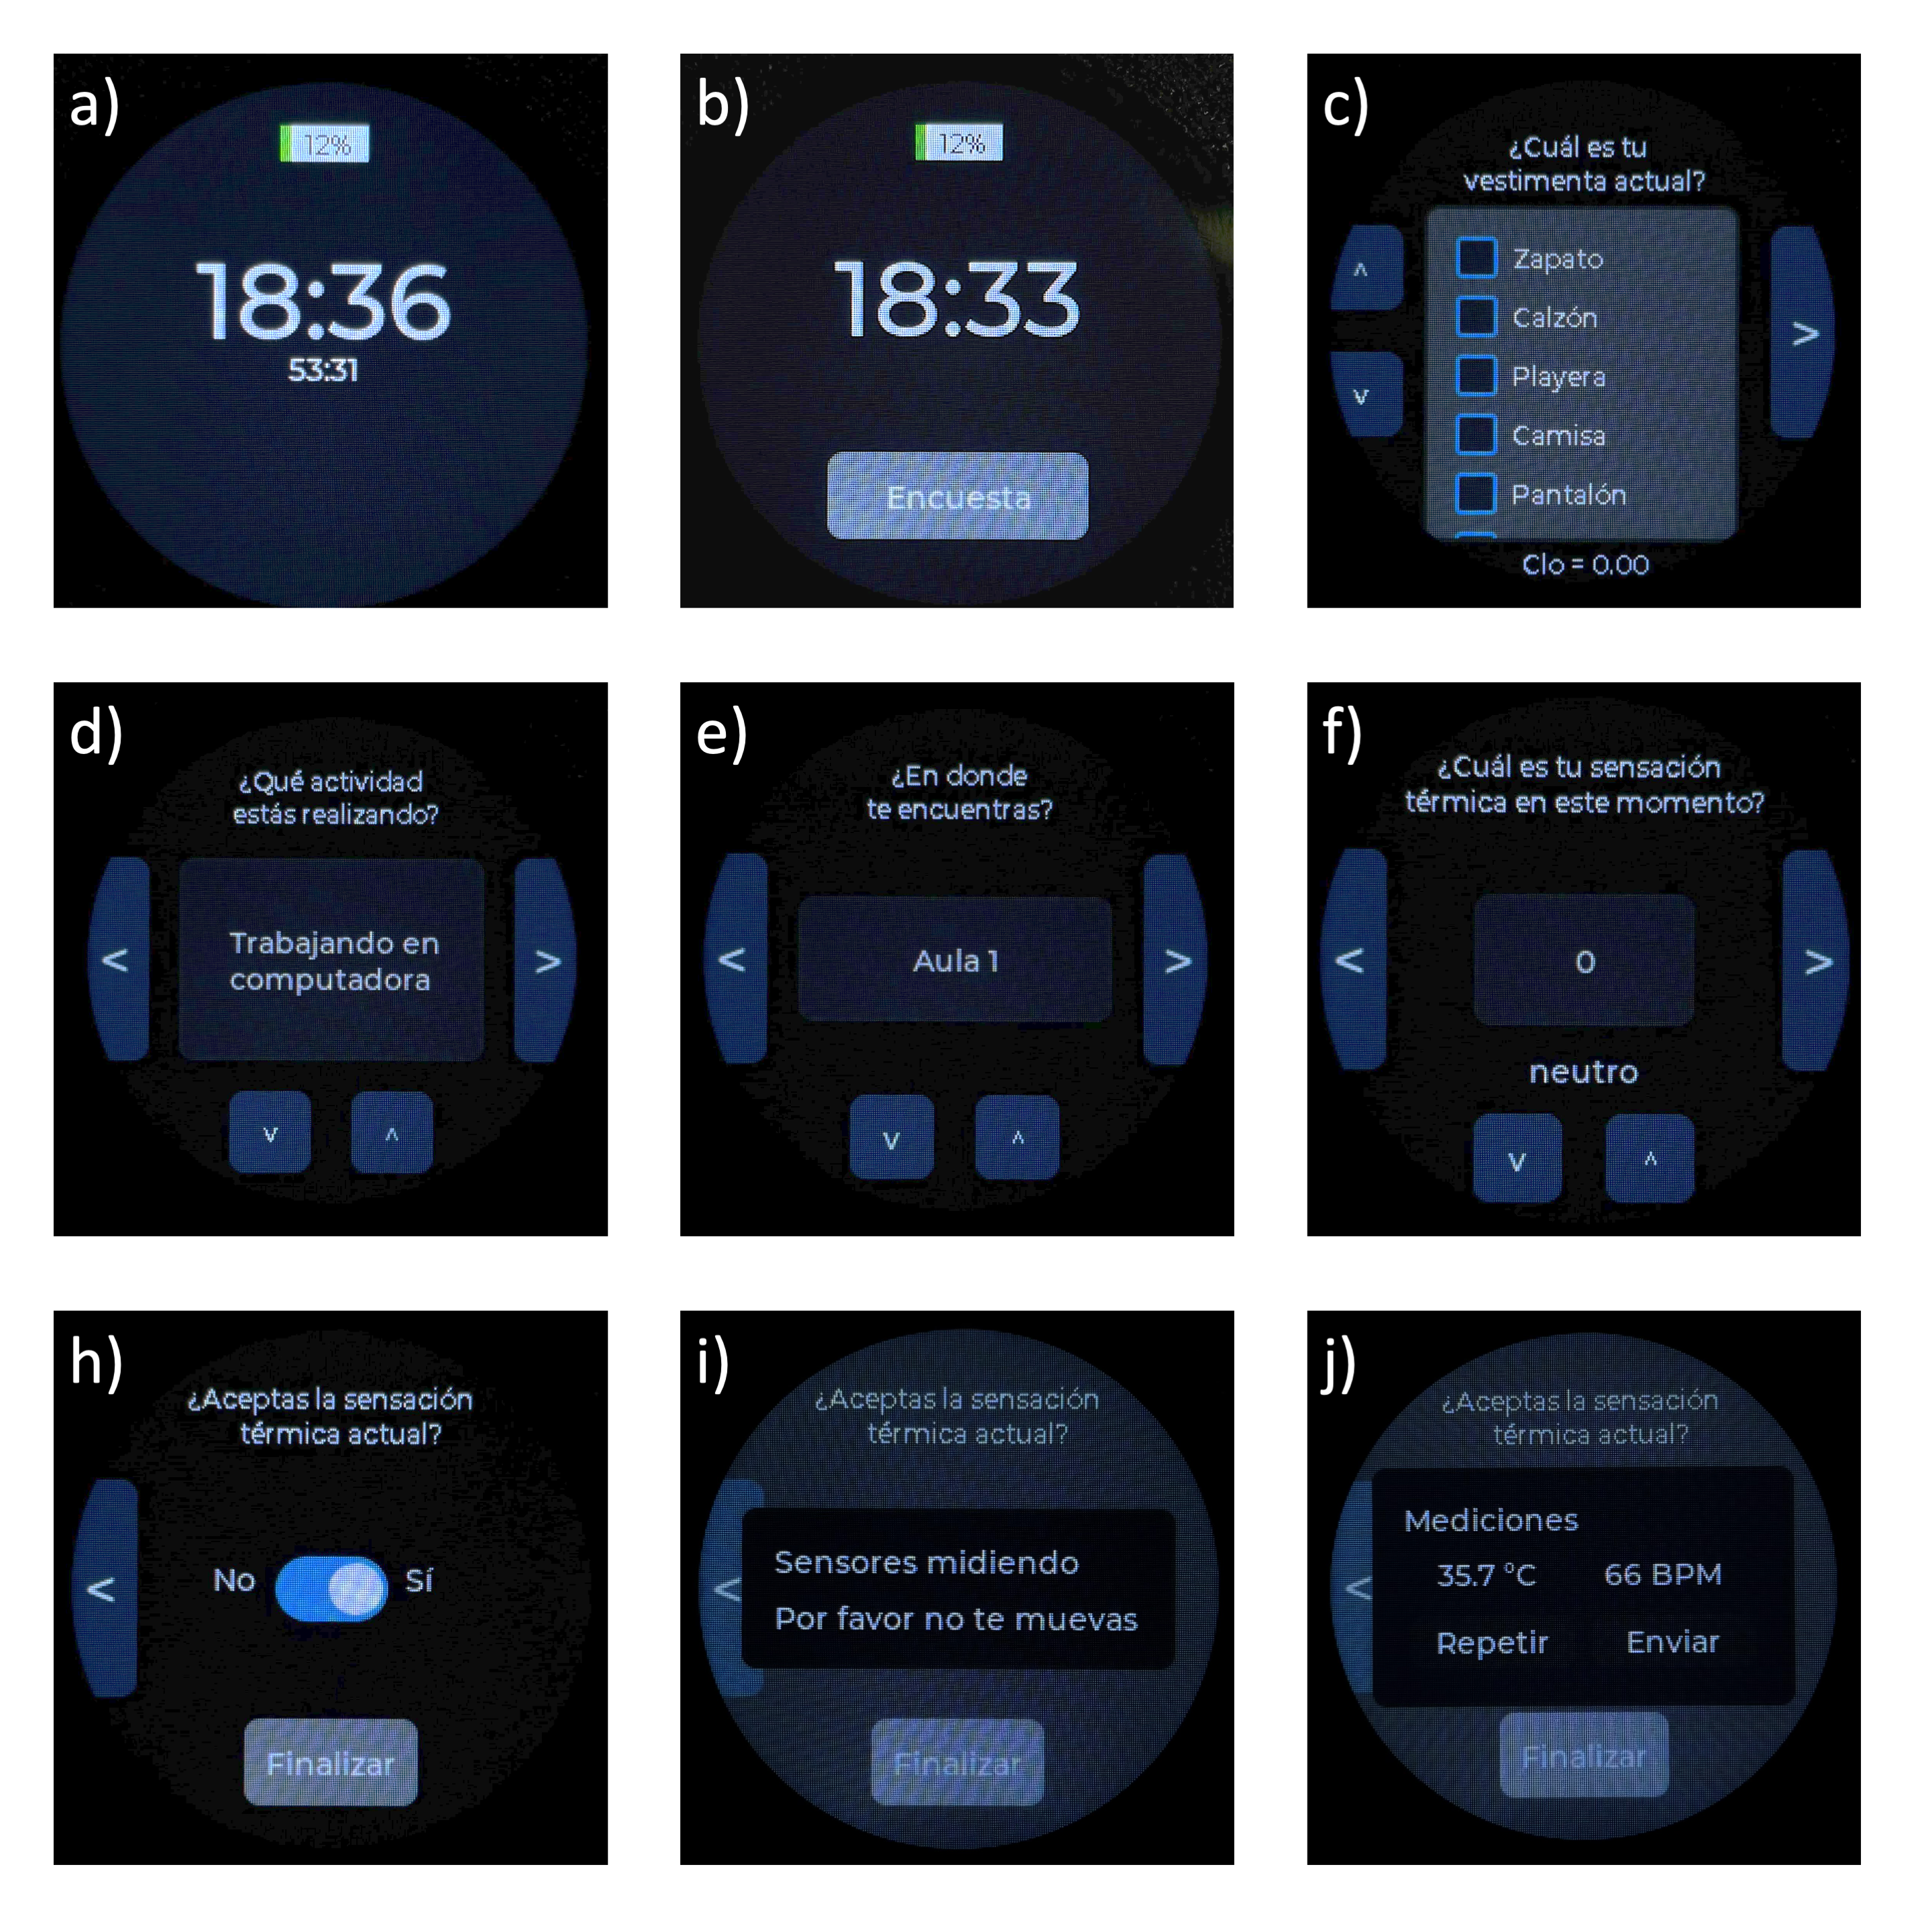
\includegraphics{Capitulos/../Imagenes/Pantallas.png}

}

\caption{\label{fig-pantallas}Interfaz del reloj inteligente: (a)
pantalla principal, (b) activación de la encuesta, (c) pregunta sobre la
vestimenta actual, (d) pregunta sobre la actividad realizada, (e)
pregunta sobre la ubicación, (f) pregunta sobre la sensación térmica,
(h) pregunta sobre la aceptación de la sensación térmica, (i) ventana
emergente indicando el inicio de las mediciones, y (j) ventana emergente
con los resultados de las mediciones.}

\end{figure}

\hypertarget{sec-validaciuxf3n}{%
\section{Validación del funcionamiento del reloj
inteligente}\label{sec-validaciuxf3n}}

Los datos generados por el reloj inteligente se almacenan en la
plataforma ThingsBoard, desde donde pueden descargarse para su posterior
análisis. Para facilitar este proceso, se diseña una libreta de Jupyter,
disponible en la carpeta descarga\_thingsboard del repositorio. Esta
libreta, denominada \texttt{Descarga\_datos.ipynb}, está programada en
Python y requiere realizar configuraciones previas para su ejecución.

\textbf{Requisitos previos}

Es necesario instalar la herramienta \texttt{git}, la cual puede
descargarse desde el siguiente enlace: descarga git. Asimismo, se
requiere la instalación de las siguientes librerías de Python:
\texttt{matplotlib}, \texttt{datetime}, \texttt{pandas} e
\texttt{iertools}. Esta ultima puede instalarse mediante el comando:

\begin{Shaded}
\begin{Highlighting}[]
\ExtensionTok{pip}\NormalTok{ install git+https://github.com/AltamarMx/iertools.git}
\end{Highlighting}
\end{Shaded}

Además, es necesario contar con el archivo \texttt{.xlsx} generado a
partir del formulario completado con la información del usuario.

Con las librerías instaladas, se procede a configurar el archivo
\texttt{config.ini}, en el cual deben ingresarse las credenciales del
dispositivo y de la plataforma ThingsBoard. Los parámetros a configurar
en este archivo son los siguientes:

\begin{itemize}
\tightlist
\item
  \textbf{dispositivo:} Nombre del dispositivo, utilizado para
  identificarlo en la libreta
\item
  \textbf{token:} Token del dispositivo en ThingsBoard
\item
  \textbf{device\_id:} ID del dispositivo
\item
  \textbf{tenant:} Cuenta de usuario en ThingsBoard
\item
  \textbf{password:} Contraseña de la cuenta
\item
  \textbf{host:} Dirección del servidor de ThingsBoard
\item
  \textbf{port:} Puerto del servidor
\end{itemize}

\textbf{Configuración de la libreta}

Dentro de la libreta \texttt{Descarga\_datos.ipynb}, se debe indicar:

\begin{itemize}
\tightlist
\item
  La ruta de ubicación del archivo \texttt{.xlsx} del formulario, como
  se muestra a continuación:
\end{itemize}

\begin{Shaded}
\begin{Highlighting}[]
\NormalTok{formulario }\OperatorTok{=} \StringTok{\textquotesingle{}../data/Formulario.xlsx\textquotesingle{}}         
\end{Highlighting}
\end{Shaded}

\begin{itemize}
\tightlist
\item
  El nombre del dispositivo, tal como está definido en el archivo
  \texttt{config.ini}:
\end{itemize}

\begin{Shaded}
\begin{Highlighting}[]
\NormalTok{nombre\_dispositivo }\OperatorTok{=} \StringTok{\textquotesingle{}Nombre del dispositivo\textquotesingle{}}   
\end{Highlighting}
\end{Shaded}

\begin{itemize}
\tightlist
\item
  El rango de fechas para la descarga de datos:
\end{itemize}

\begin{Shaded}
\begin{Highlighting}[]
\NormalTok{fecha1 }\OperatorTok{=}\NormalTok{ parse(}\StringTok{"2024{-}01{-}01"}\NormalTok{)  }
\NormalTok{fecha2 }\OperatorTok{=}\NormalTok{ datetime.datetime.now()}
\end{Highlighting}
\end{Shaded}

\textbf{Descarga y procesamiento de datos}

Una vez configurada la libreta, se realiza la descarga de los datos
almacenados en ThingsBoard dentro del rango de fechas especificado.
Posteriormente, se genera un dataframe que combina estas mediciones con
las respuestas obtenidas del formulario. Este proceso permite validar
que el dispositivo es capaz de registrar encuestas, medir variables
fisiológicas y envíar correctamente los datos a ThingsBoard para su
almacenamiento.

\textbf{Resultados de la validación}

Para validar el funcionamiento del reloj inteligente, se realizan dos
campañas de medición, cada una con diferentes individuos, obteniendo un
total de 60 mediciones. La Tabla~\ref{tbl-data_downloaded} proporciona
una muestra que incluye tres mediciones correspondientes al primer
sujeto y tres mediciones del segundo sujeto.

En la tabla, la columna correspondiente a la frecuencia de uso de
espacios con aire acondicionado (\(F\)) se muestra de forma numérica.
Esto se debe a que los valores de esta columna están codificados según
un diccionario, cuyo propósito es simplificar la visualización de los
datos. La equivalencia de este diccionario es la siguiente:

\begin{Shaded}
\begin{Highlighting}[]
\NormalTok{diccionario\_frecuencia }\OperatorTok{=}\NormalTok{ \{}
    \StringTok{"Todos los días"}\NormalTok{: }\DecValTok{3}\NormalTok{,}
    \StringTok{"3 a 5 días a la semana"}\NormalTok{: }\DecValTok{2}\NormalTok{,}
    \StringTok{"1 a 3 días a la semana"}\NormalTok{: }\DecValTok{1}\NormalTok{,}
    \StringTok{"Nunca"}\NormalTok{: }\DecValTok{0}
\NormalTok{\}}
\end{Highlighting}
\end{Shaded}

\hypertarget{tbl-data_downloaded}{}
\begin{longtable}[]{@{}
  >{\raggedright\arraybackslash}p{(\columnwidth - 26\tabcolsep) * \real{0.1196}}
  >{\raggedright\arraybackslash}p{(\columnwidth - 26\tabcolsep) * \real{0.0815}}
  >{\raggedright\arraybackslash}p{(\columnwidth - 26\tabcolsep) * \real{0.0652}}
  >{\raggedright\arraybackslash}p{(\columnwidth - 26\tabcolsep) * \real{0.0870}}
  >{\raggedright\arraybackslash}p{(\columnwidth - 26\tabcolsep) * \real{0.0543}}
  >{\raggedright\arraybackslash}p{(\columnwidth - 26\tabcolsep) * \real{0.0489}}
  >{\raggedright\arraybackslash}p{(\columnwidth - 26\tabcolsep) * \real{0.0761}}
  >{\raggedright\arraybackslash}p{(\columnwidth - 26\tabcolsep) * \real{0.0652}}
  >{\raggedright\arraybackslash}p{(\columnwidth - 26\tabcolsep) * \real{0.0598}}
  >{\raggedright\arraybackslash}p{(\columnwidth - 26\tabcolsep) * \real{0.0543}}
  >{\raggedright\arraybackslash}p{(\columnwidth - 26\tabcolsep) * \real{0.0543}}
  >{\raggedright\arraybackslash}p{(\columnwidth - 26\tabcolsep) * \real{0.0598}}
  >{\raggedright\arraybackslash}p{(\columnwidth - 26\tabcolsep) * \real{0.0543}}
  >{\raggedright\arraybackslash}p{(\columnwidth - 26\tabcolsep) * \real{0.0543}}@{}}
\caption{\label{tbl-data_downloaded}Conjunto de datos de cinco encuestas
térmicas y mediciones, que incluye el nivel de aislamiento de la ropa
(\(I_{cl}\)), la tasa metabólica (\(M_r\)), la ubicación, el voto de
sensación térmica (TSV), la aceptación térmica (TA), la temperatura de
la piel de la muñeca (\(T_w\)), la frecuencia cardíaca (\(H_r\)), la
edad, el peso (\(W\)), la altura (\(H\)), el sexo, la frecuencia de uso
de espacios con aire acondicionado (\(F\)) y el identificador del
individuo que está usando el reloj inteligente (\(I\)).}\tabularnewline
\toprule\noalign{}
\multirow{4}{*}{\begin{minipage}[b]{\linewidth}\raggedright
\textbf{Fecha}

\emph{AAAA-MM-DD HH:MM}
\end{minipage}} &
\multirow{4}{*}{\begin{minipage}[b]{\linewidth}\raggedright
\textbf{\(I_{cl}\)}

\emph{clo}
\end{minipage}} &
\multirow{4}{*}{\begin{minipage}[b]{\linewidth}\raggedright
\textbf{\(M_r\)}

\emph{met}
\end{minipage}} &
\multirow{4}{*}{\begin{minipage}[b]{\linewidth}\raggedright
\textbf{Ubicación}

\emph{-}
\end{minipage}} &
\multirow{4}{*}{\begin{minipage}[b]{\linewidth}\raggedright
\textbf{TSV}

\emph{-}
\end{minipage}} &
\multirow{4}{*}{\begin{minipage}[b]{\linewidth}\raggedright
\textbf{TA}

\emph{-}
\end{minipage}} &
\multirow{4}{*}{\begin{minipage}[b]{\linewidth}\raggedright
\textbf{\(T_{w}\)}

\emph{°C}
\end{minipage}} &
\multirow{4}{*}{\begin{minipage}[b]{\linewidth}\raggedright
\textbf{\(H_r\)}

\emph{bpm}
\end{minipage}} &
\multirow{4}{*}{\begin{minipage}[b]{\linewidth}\raggedright
\textbf{Edad}

\emph{años}
\end{minipage}} &
\multirow{4}{*}{\begin{minipage}[b]{\linewidth}\raggedright
\textbf{\(W\)}

\emph{kg}
\end{minipage}} &
\multirow{4}{*}{\begin{minipage}[b]{\linewidth}\raggedright
\textbf{\(H\)}

\emph{m}
\end{minipage}} &
\multirow{4}{*}{\begin{minipage}[b]{\linewidth}\raggedright
\textbf{Sexo}

\emph{-}
\end{minipage}} &
\multirow{4}{*}{\begin{minipage}[b]{\linewidth}\raggedright
\textbf{\(F\)}

\emph{-}
\end{minipage}} &
\multirow{4}{*}{\begin{minipage}[b]{\linewidth}\raggedright
\textbf{\(I\)}

\emph{-}
\end{minipage}} \\
 \\
 \\
 \\
\midrule\noalign{}
\endfirsthead
\toprule\noalign{}
\multirow{4}{*}{\begin{minipage}[b]{\linewidth}\raggedright
\textbf{Fecha}

\emph{AAAA-MM-DD HH:MM}
\end{minipage}} &
\multirow{4}{*}{\begin{minipage}[b]{\linewidth}\raggedright
\textbf{\(I_{cl}\)}

\emph{clo}
\end{minipage}} &
\multirow{4}{*}{\begin{minipage}[b]{\linewidth}\raggedright
\textbf{\(M_r\)}

\emph{met}
\end{minipage}} &
\multirow{4}{*}{\begin{minipage}[b]{\linewidth}\raggedright
\textbf{Ubicación}

\emph{-}
\end{minipage}} &
\multirow{4}{*}{\begin{minipage}[b]{\linewidth}\raggedright
\textbf{TSV}

\emph{-}
\end{minipage}} &
\multirow{4}{*}{\begin{minipage}[b]{\linewidth}\raggedright
\textbf{TA}

\emph{-}
\end{minipage}} &
\multirow{4}{*}{\begin{minipage}[b]{\linewidth}\raggedright
\textbf{\(T_{w}\)}

\emph{°C}
\end{minipage}} &
\multirow{4}{*}{\begin{minipage}[b]{\linewidth}\raggedright
\textbf{\(H_r\)}

\emph{bpm}
\end{minipage}} &
\multirow{4}{*}{\begin{minipage}[b]{\linewidth}\raggedright
\textbf{Edad}

\emph{años}
\end{minipage}} &
\multirow{4}{*}{\begin{minipage}[b]{\linewidth}\raggedright
\textbf{\(W\)}

\emph{kg}
\end{minipage}} &
\multirow{4}{*}{\begin{minipage}[b]{\linewidth}\raggedright
\textbf{\(H\)}

\emph{m}
\end{minipage}} &
\multirow{4}{*}{\begin{minipage}[b]{\linewidth}\raggedright
\textbf{Sexo}

\emph{-}
\end{minipage}} &
\multirow{4}{*}{\begin{minipage}[b]{\linewidth}\raggedright
\textbf{\(F\)}

\emph{-}
\end{minipage}} &
\multirow{4}{*}{\begin{minipage}[b]{\linewidth}\raggedright
\textbf{\(I\)}

\emph{-}
\end{minipage}} \\
 \\
 \\
 \\
\midrule\noalign{}
\endhead
\bottomrule\noalign{}
\endlastfoot
\multirow{2}{*}{2024-07-17 13:32} & \multirow{2}{*}{0.21} &
\multirow{2}{*}{1.5} & \multirow{2}{*}{Aula 1} & \multirow{2}{*}{0.0} &
\multirow{2}{*}{Sí} & \multirow{2}{*}{34.3} & \multirow{2}{*}{66} &
\multirow{2}{*}{28} & \multirow{2}{*}{65} & \multirow{2}{*}{1.70} &
\multirow{2}{*}{M} & \multirow{2}{*}{1} & \multirow{2}{*}{1} \\
 \\
\multirow{2}{*}{2024-07-17 14:32} & \multirow{2}{*}{0.21} &
\multirow{2}{*}{1.5} & \multirow{2}{*}{Aula 1} & \multirow{2}{*}{0.0} &
\multirow{2}{*}{Sí} & \multirow{2}{*}{35.4} & \multirow{2}{*}{77} &
\multirow{2}{*}{28} & \multirow{2}{*}{65} & \multirow{2}{*}{1.70} &
\multirow{2}{*}{M} & \multirow{2}{*}{1} & \multirow{2}{*}{1} \\
 \\
\multirow{2}{*}{2024-07-17 16:45} & \multirow{2}{*}{0.21} &
\multirow{2}{*}{2.0} & \multirow{2}{*}{Aula 1} & \multirow{2}{*}{2.0} &
\multirow{2}{*}{No} & \multirow{2}{*}{35.2} & \multirow{2}{*}{85} &
\multirow{2}{*}{28} & \multirow{2}{*}{65} & \multirow{2}{*}{1.70} &
\multirow{2}{*}{M} & \multirow{2}{*}{1} & \multirow{2}{*}{1} \\
 \\
\multirow{2}{*}{\ldots{}} & \multirow{2}{*}{\ldots{}} &
\multirow{2}{*}{\ldots{}} & \multirow{2}{*}{\ldots{}} &
\multirow{2}{*}{\ldots{}} & \multirow{2}{*}{\ldots{}} &
\multirow{2}{*}{\ldots{}} & \multirow{2}{*}{\ldots{}} &
\multirow{2}{*}{\ldots{}} & \multirow{2}{*}{\ldots{}} &
\multirow{2}{*}{\ldots{}} & \multirow{2}{*}{\ldots{}} &
\multirow{2}{*}{\ldots{}} & \multirow{2}{*}{\ldots{}} \\
 \\
\multirow{2}{*}{2024-11-13 08:46} & \multirow{2}{*}{0.48} &
\multirow{2}{*}{1.3} & \multirow{2}{*}{Aula 2} & \multirow{2}{*}{0.0} &
\multirow{2}{*}{Sí} & \multirow{2}{*}{33.6} & \multirow{2}{*}{62} &
\multirow{2}{*}{46} & \multirow{2}{*}{73} & \multirow{2}{*}{1.70} &
\multirow{2}{*}{M} & \multirow{2}{*}{1} & \multirow{2}{*}{2} \\
 \\
\multirow{2}{*}{2024-11-14 16:45} & \multirow{2}{*}{0.40} &
\multirow{2}{*}{1.3} & \multirow{2}{*}{Aula 2} & \multirow{2}{*}{0.0} &
\multirow{2}{*}{Sí} & \multirow{2}{*}{36.9} & \multirow{2}{*}{64} &
\multirow{2}{*}{46} & \multirow{2}{*}{73} & \multirow{2}{*}{1.70} &
\multirow{2}{*}{M} & \multirow{2}{*}{1} & \multirow{2}{*}{2} \\
 \\
\multirow{2}{*}{2024-11-14 20:45} & \multirow{2}{*}{0.40} &
\multirow{2}{*}{1.3} & \multirow{2}{*}{Aula 2} & \multirow{2}{*}{0.0} &
\multirow{2}{*}{Sí} & \multirow{2}{*}{35.0} & \multirow{2}{*}{93} &
\multirow{2}{*}{46} & \multirow{2}{*}{70} & \multirow{2}{*}{1.70} &
\multirow{2}{*}{M} & \multirow{2}{*}{1} & \multirow{2}{*}{2} \\
 \\
\end{longtable}

En la Figura~\ref{fig-relojfuncionando}, se observa el dispositivo en
funcionamiento. El reloj se ajusta en la muñeca del usuario y muestra la
interfaz principal con la hora actual y el estado de la batería.

\begin{figure}

{\centering \includegraphics[width=0.5\textwidth,height=\textheight]{Capitulos/../Imagenes/Reloj-funcionando.jpg}

}

\caption{\label{fig-relojfuncionando}Reloj inteligente en
funcionamiento, mostrando la interfaz principal.}

\end{figure}

\bookmarksetup{startatroot}

\hypertarget{conclusiones}{%
\chapter{Conclusiones}\label{conclusiones}}

Este proyecto presenta el diseño, desarrollo y validación de un reloj
inteligente basado en tecnologías abiertas, capaz de recopilar datos de
confort térmico. El reloj realiza encuestas simplificadas y mide
variables fisiológicas como la temperatura de la piel y la frecuencia
cardíaca, integrando esta información con la plataforma IoT ThingsBoard.
El uso de hardware de código abierto, como la placa de desarrollo XIAO
ESP32C3 y los sensores GY-906 (temperatura de la piel) y MAX30102
(frecuencia cardíaca) garantiza que el dispositivo sea replicable y
adaptable a diversas investigaciones. Además, el reloj cuenta con una
alarma vibrante que notifica al usuario cuando debe responder una nueva
encuesta, promoviendo la regularidad y periodicidad en la recopilación
de datos. En pruebas realizadas en Temixco, Morelos, el reloj logró
recopilar y enviar cincuenta y dos mediciones a ThingsBoard en una
campaña de cinco días, demostrando su funcionalidad en condiciones
reales.

\hypertarget{contribuciones-del-proyecto}{%
\section{Contribuciones del
proyecto}\label{contribuciones-del-proyecto}}

\begin{enumerate}
\def\labelenumi{\arabic{enumi}.}
\tightlist
\item
  \textbf{Diseño basado en tecnologías abiertas}
\end{enumerate}

El reloj inteligente se desarrolla por completo utilizando tecnologías
abiertas, tanto en hardware como en software. Para el hardware, el
dispositivo integra componentes como la placa de desarrollo XIAO
ESP32C3, el sensor MAX30102, el sensor GY-906, la pantalla XIAO Round
Display, y otros componentes electrónicos. Para el software, el
dispositivo se programa utilizando Arduino IDE, empleando lenguajes de
programación como Arduino y C++. Los datos recopilados se envían a
ThingsBoard, una plataforma de Internet de las Cosas (IoT, por sus
siglas en inglés) de código abierto, para su almacenamiento.

Todo el proyecto se encuentra disponible en un repositorio de GitHub
bajo la licencia GPL-3.0, lo que garantiza que cualquier persona pueda
replicar, modificar o colaborar en el desarrollo del dispositivo,
fomentando la accesibilidad y colaboración en investigaciones futuras
relacionadas con el confort térmico.

\begin{enumerate}
\def\labelenumi{\arabic{enumi}.}
\setcounter{enumi}{1}
\tightlist
\item
  \textbf{Uso en condiciones reales}
\end{enumerate}

El reloj inteligente está diseñado para realizar campañas de medición
prolongadas en condiciones reales, recolectando datos de usuarios en sus
entornos habituales sin la necesidad de equipos complejos. Para
facilitar la recolección de datos de manera periódica, el reloj incluye
una alarma vibrante que notifica al usuario cuando es momento de
responder una encuesta simplificada de confort térmico. Los datos
recopilados por el reloj se combinan con información proporcionada en el
formulario de registro generando una base de datos contextualizada que
permite correlacionar las respuestas del usuario con las condiciones
ambientales reales.

\begin{enumerate}
\def\labelenumi{\arabic{enumi}.}
\setcounter{enumi}{2}
\tightlist
\item
  \textbf{Bajo costo}
\end{enumerate}

El desarrollo del reloj inteligente basado en tecnologías abiertas ha
permitido implementar funcionalidades similares a las ofrecidas por
combinaciones de dispositivos comerciales y aplicaciones existentes a un
costo aproximado de \$1,120 MXN. La aplicación Cozie, si bien ofrece una
solución para el levantamiento de encuestas en relojes inteligentes, su
uso está restringido a los Apple Watch y algunos modelos de Fitbit.
Además, estos dispositivos tienen un costo elevado. El Apple Watch
Series 8 (Apple Watch más económico que incluye sensor de temperatura)
tiene un precio aproximado en el mercado al momento de la publicación de
esta tesis de \$5,500 MXN, mientras que, el Fitbit Versa 4 (compatible
con Cozie) tiene un precio aproximado al momento de la publicación de
esta tesis de \$4,200 MXN. Existen dispositivos más económicos como el
Fitbit Inspire 3 por un precio aproximado de \$2,000 MXN que cumplen con
la función de medir la frecuencia cardíaca y la temperatura de la piel,
sin embargo no cuenta con la funcionalidad de realizar encuestas.

El reloj desarrollado en este proyecto, tiene un costo aproximado de
\$1,120 MXN e integra las capacidades de medición de variables
fisiológicas y realización de encuestas. Esto lo convierte en una opción
accesible y funcional.

\begin{enumerate}
\def\labelenumi{\arabic{enumi}.}
\setcounter{enumi}{3}
\tightlist
\item
  \textbf{Adaptabilidad}
\end{enumerate}

El reloj inteligente cuenta con un diseño que permite su adaptación a
diversas aplicaciones además de las encuestas de confort térmico. Puede
configurarse para implementar otros tipos de encuestas o funcionalidades
específicas según las necesidades del proyecto. Además, al estar
desarrollado en Arduino sobre un microcontrolador ESP32 y emplear la
biblioteca LVGL, ofrece la posibilidad de migrar su software a
MicroPython, ampliando su versatilidad.

\hypertarget{limitantes-del-proyecto}{%
\section{Limitantes del proyecto}\label{limitantes-del-proyecto}}

A pesar de los logros alcanzados, el proyecto enfrenta algunas
limitantes:

\begin{enumerate}
\def\labelenumi{\arabic{enumi}.}
\tightlist
\item
  \textbf{Precisión de los sensores de bajo costo}
\end{enumerate}

Los sensores utilizados son sensores comerciales de bajo costo, que si
bien cumplen con la funcionalidad requerida, se pueden ver afectados en
términos de exactitud. Aunque estos sensores fueron sometidos a un
proceso de calibración para disminuir errores, las mediciones podrían
mejorarse con sensores de mayor exactitud, aunque eso implicaría un
costo más elevado del reloj.

\begin{enumerate}
\def\labelenumi{\arabic{enumi}.}
\setcounter{enumi}{1}
\tightlist
\item
  \textbf{Ergonomía del reloj inteligente}
\end{enumerate}

El diseño actual del reloj inteligente lo convierte en un dispositivo
grande para un reloj, lo cual puede resultar incomodo para algunos
usuarios durante su uso de manera prolongada. Además, la carcasa
presenta cierta fragilidad al no estar diseñada para impactos o
condiciones adversas.

\hypertarget{trabajo-futuro}{%
\section{Trabajo futuro}\label{trabajo-futuro}}

El desarrollo del reloj inteligente plantea diversas oportunidades para
extender su funcionalidad y aplicabilidad:

\begin{enumerate}
\def\labelenumi{\arabic{enumi}.}
\tightlist
\item
  \textbf{Integración con el ecosistema del IER}
\end{enumerate}

Una de las principales tareas de trabajo a futuro es la integración del
reloj inteligente al ecosistema de dispositivos del IER, que incluye la
estación meteorológica ESOLMET y los distintos dispositivos en
desarrollo en el Laboratorio de Tecnologías Abiertas y Más (LATA+). La
integración del reloj con este ecosistema permitirá generar una base de
datos amplia y contextualizada para Temixco, Morelos. Así como también
permitirá la correlación de diferentes variables para el análisis de
confort térmico.

\begin{enumerate}
\def\labelenumi{\arabic{enumi}.}
\setcounter{enumi}{1}
\tightlist
\item
  \textbf{Campañas prolongadas de medición}
\end{enumerate}

Para generar una base de datos amplia representativa sobre confort
térmico en Temixco, Morelos, es necesario llevar a cabo campañas de
medición durante varios meses con la participación de distintos
usuarios. Para ello se requiere la fabricación de un mayor número de
relojes inteligentes. A largo plazo, esta estrategia contribuirá el
estudio del confort térmico en Temixco, Morelos, y en otros lugares
donde se adopte el uso de este reloj inteligente.

\begin{enumerate}
\def\labelenumi{\arabic{enumi}.}
\setcounter{enumi}{2}
\tightlist
\item
  \textbf{Desarrollo de modelos de confort térmico}
\end{enumerate}

La creación de una base de datos amplia y contextualizada abre la
posibilidad al desarrollo de modelos de confort térmico adaptativos a
contextos específicos, como el bioclima cálido subhúmedo característico
de Temixco. Estos modelos podrían integrar variables ambientales como
temperatura, humedad relativa y velocidad del viento, tomadas desde la
estación meteorológica ESOLMET o los dispositivos desarrollados en el
IER, junto con las variables fisiológicas tomadas por el reloj
inteligente y datos obtenidos del formulario, tales como la edad, sexo,
peso, altura y frecuencia de uso de aire acondicionado.

\begin{enumerate}
\def\labelenumi{\arabic{enumi}.}
\setcounter{enumi}{3}
\tightlist
\item
  \textbf{Mejoras en los sensores}
\end{enumerate}

El diseño modular del reloj facilita la búsqueda e integración de
sensores de mayor calidad que puedan reemplazar a los sensores actuales
para facilitar el proceso de calibración, aumentar la exactitud y
precisión de las lecturas, y mejorar la fiabilidad de los datos
recopilados.

\begin{enumerate}
\def\labelenumi{\arabic{enumi}.}
\setcounter{enumi}{4}
\tightlist
\item
  \textbf{Mejoras en el diseño de la carcasa}
\end{enumerate}

La carcasa del reloj inteligente puede mejorarse con la aplicación de
conocimientos en diseño industrial e impresión 3D. Estas mejoras
permitirían reducir el tamaño del dispositivo, hacerlo más cómodo y
aumentar su resistencia a condiciones adversas.

\hypertarget{conclusiuxf3n-general}{%
\section{Conclusión general}\label{conclusiuxf3n-general}}

El reloj inteligente desarrollado en este proyecto demuestra cómo las
tecnologías abiertas pueden utilizarse para crear herramientas
funcionales destinadas a la investigación, en este caso especifico, en
el campo del confort térmico. La simplicidad del diseño lo convierte en
una solución viable para estudios de confort térmico en ambientes
reales. Aunado a su capacidad para la recolección de datos de manera
eficiente a través de la conexión a internet con una plataforma de IoT,
abre la posibilidad de desarrollar modelos de confort térmico
adaptativos.

No obstante, el dispositivo enfrenta algunos retos a superar, como
mejorar la exactitud de los sensores y mejorar el diseño y resistencia
de la carcasa.

La integración del reloj inteligente al ecosistema del IER, así como las
campañas de recolección de datos para la creación de bases de datos
contextualizadas, permitirá a largo plazo correlacionar variables
ambientales y fisiológicas para llevar a cabo estudios de confort
térmico. El Desarrollo de modelos de confort adaptativos basados en
estas bases de datos no solo contribuirá al estudio del confort térmico
de manera general, sino que también servirá como base para el desarrollo
de estrategias de diseño bioclimático especificas para regiones con
bioclimas cálidos subhúmedos.

Este proyecto aporta una herramienta accesible para el ámbito de la
investigación, al tiempo que abre nuevos retos y oportunidades de
colaboración interdisciplinaria y de desarrollo tecnológico. Además, se
alinea con la filosofía de las tecnologías abiertas, promoviendo su uso
en beneficio de la comunidad científica y fomentando la transparencia,
la colaboración y el acceso a herramientas que impulsen nuevas
investigaciones.

\bookmarksetup{startatroot}

\hypertarget{referencias}{%
\chapter*{Referencias}\label{referencias}}
\addcontentsline{toc}{chapter}{Referencias}

\markboth{Referencias}{Referencias}

\hypertarget{refs}{}
\begin{CSLReferences}{1}{0}
\leavevmode\vadjust pre{\hypertarget{ref-Calixto2021}{}}%
Aguirre, Verónica Ivette Calixto. 2021. {«Thermal comfort studies»}.
Universidad Nacional Autonoma de México.
\url{http://132.248.9.195/ptd2021/septiembre/0814603/Index.html}.

\leavevmode\vadjust pre{\hypertarget{ref-ASHRAE2009}{}}%
American Society of Heating, Refrigerating and Air-Conditioning
Engineers. 2009. \emph{ASHRAE Handbook---Fundamentals (SI Edition)}.
Atlanta, GA: ASHRAE.

\leavevmode\vadjust pre{\hypertarget{ref-ASHRAE55}{}}%
American Society of Heating, Refrigerating and Air-Conditioning
Engineers, Inc. 2017. \emph{Thermal Environmental Conditions for Human
Occupancy}. ASHRAE Standard 55-2017. American Society of Heating,
Refrigerating; Air-Conditioning Engineers, Inc.

\leavevmode\vadjust pre{\hypertarget{ref-Bogatu2023}{}}%
Bogatu, Dragos Ioan, Jun Shinoda, José Joaquín Aguilera, Bjarne W.
Olesen, Futa Watanabe, Yosuke Kaneko, y Ongun B. Kazanci. 2023. {«Human
physiology for personal thermal comfort-based HVAC control -- A
review»}. \emph{Building and Environment} 240 (julio): 110418.
\url{https://doi.org/10.1016/J.BUILDENV.2023.110418}.

\leavevmode\vadjust pre{\hypertarget{ref-chao_cen__2023}{}}%
Cen, Chao, Siyu Cheng, y Nyuk Hien Wong. 2023. {«Effect of elevated air
temperature and air velocity on thermal comfort and cognitive
performance in the tropics»}. \emph{Building and Environment} 234:
110203-3.
\href{https://doi.org/\%2010.1016/j.buildenv.2023.110203\%20}{https://doi.org/
10.1016/j.buildenv.2023.110203 }.

\leavevmode\vadjust pre{\hypertarget{ref-Chaudhuri2020}{}}%
Chaudhuri, Tanaya, Yeng Chai Soh, Hua Li, y Lihua Xie. 2020. {«Machine
learning driven personal comfort prediction by wearable sensing of pulse
rate and skin temperature»}. \emph{Building and Environment} 170
(marzo): 106615. \url{https://doi.org/10.1016/j.buildenv.2019.106615}.

\leavevmode\vadjust pre{\hypertarget{ref-Chaudhuri2018}{}}%
Chaudhuri, Tanaya, Deqing Zhai, Yeng Chai Soh, Hua Li, y Lihua Xie.
2018. {«Random forest based thermal comfort prediction from
gender-specific physiological parameters using wearable sensing
technology»}. \emph{Energy and Buildings} 166 (mayo): 391-406.
\url{https://doi.org/10.1016/J.ENBUILD.2018.02.035}.

\leavevmode\vadjust pre{\hypertarget{ref-Cho2023}{}}%
Cho, Seonghun, Hong Jae Nam, Chuanqi Shi, Choong Yeon Kim, Sang-Hyuk
Byun, Karen-Christian Agno, Byung Chul Lee, Jianliang Xiao, Joo Yong
Sim, y Jae-Woong Jeong. 2023. {«Wireless, AI-enabled wearable thermal
comfort sensor for energy-efficient, human-in-the-loop control of indoor
temperature»}. \emph{Biosensors and Bioelectronics} 223 (marzo): 115018.
\url{https://doi.org/10.1016/j.bios.2022.115018}.

\leavevmode\vadjust pre{\hypertarget{ref-Choi2017}{}}%
Choi, Joon Ho, y Dongwoo Yeom. 2017. {«Study of data-driven thermal
sensation prediction model as a function of local body skin temperatures
in a built environment»}. \emph{Building and Environment} 121 (agosto):
130-47. \url{https://doi.org/10.1016/J.BUILDENV.2017.05.004}.

\leavevmode\vadjust pre{\hypertarget{ref-OTD_Roadmap_Plan}{}}%
Departamento de Defensa de EE.UU. 2009. {«{Desarrollo de Tecnología
Abierta: Lecciones aprendidas y mejores prácticas para software
militar}»}.
\url{https://dodcio.defense.gov/Portals/0/Documents/FOSS/OTD-lessons-learned-military-signed.pdf}.

\leavevmode\vadjust pre{\hypertarget{ref-Enescu2017}{}}%
Enescu, Diana. 2017. {«A review of thermal comfort models and indicators
for indoor environments»}. \emph{Renewable and Sustainable Energy
Reviews} 79 (noviembre): 1353-79.
\url{https://doi.org/10.1016/J.RSER.2017.05.175}.

\leavevmode\vadjust pre{\hypertarget{ref-Fanger1970}{}}%
Fanger, P. O. 1970. \emph{Thermal Comfort: Analysis and Applications in
Environmental Engineering}. Copenhagen: Danish Technical Press.
\url{https://archive.org/details/thermalcomfortan0000fang}.

\leavevmode\vadjust pre{\hypertarget{ref-Fanger2002}{}}%
Fanger, P. O., y Jørn Toftum. 2002. {«Extension of the PMV model to
non-air-conditioned buildings in warm climates»}. \emph{Energy and
Buildings} 34 (6): 533-36.
https://doi.org/\url{https://doi.org/10.1016/S0378-7788(02)00003-8}.

\leavevmode\vadjust pre{\hypertarget{ref-Feng2023}{}}%
Feng, Yanxiao, Julian Wang, Nan Wang, y Chenshun Chen. 2023.
{«Alert-based wearable sensing system for individualized thermal
preference prediction»}. \emph{Building and Environment} 232 (marzo):
110047. \url{https://doi.org/10.1016/J.BUILDENV.2023.110047}.

\leavevmode\vadjust pre{\hypertarget{ref-infonavit_regiones_bioclimaticas}{}}%
Fondo Nacional de la Vivienda para los Trabajadores (Infonavit),
Instituto del. 2020. {«Anexo 1. Listado de regiones bioclimáticas»}.
\url{https://portalmx.infonavit.org.mx/wps/wcm/connect/005dcf74-d918-41aa-acfa-927e7b33d98a/12.+Anexo/\%2B1./\%2BListado/\%2Bde/\%2Bregiones/\%2Bbioclim/\%C3/\%A1ticas.pdf?MOD=AJPERES\&CONVERT_TO=url\&CACHEID=ROOTWORKSPACE-005dcf74-d918-41aa-acfa-927e7b33d98a-mmCFC0}.

\leavevmode\vadjust pre{\hypertarget{ref-Garces2021}{}}%
Garces, Hugo O., Eduardo Morales, Rodrigo Gomez, Hans Cabrera, y Eduardo
Espinosa. 2021. {«Design and calibration of low cost sensor node for
thermal comfort estimation»}. \emph{2021 29th Mediterranean Conference
on Control and Automation, MED 2021}, junio, 1215-21.
\url{https://doi.org/10.1109/MED51440.2021.9480306}.

\leavevmode\vadjust pre{\hypertarget{ref-Vero2023}{}}%
Gnecco, Veronica Martins, Ilaria Pigliautile, y Anna Laura Pisello.
2023. {«Long-Term Thermal Comfort Monitoring via Wearable Sensing
Techniques: Correlation between Environmental Metrics and Subjective
Perception»}. \emph{Sensors} 23 (enero): 576.
\url{https://doi.org/10.3390/s23020576}.

\leavevmode\vadjust pre{\hypertarget{ref-gomez-azpetia2006adaptacion}{}}%
Gómez-Azpetia, G., E. López Gómez, y M. Peña. 2006. {«Adaptaci{ó}n del
{ı́}ndice Humidex para el clima de la ciudad de Colima, M{é}xico, de
acuerdo con el enfoque adaptativo»}. \emph{Anuario} VIII: 77-92.

\leavevmode\vadjust pre{\hypertarget{ref-He2025IMU}{}}%
He, Weilin, Cheng Fan, Zebin Wu, y Qiaoqiao Yong. 2025. {«An IMU dataset
for human thermal comfort activities identification: Experimental
designs and applications»}. \emph{Energy and Built Environment} 6:
66-79. \url{https://doi.org/10.1016/j.enbenv.2023.09.001}.

\leavevmode\vadjust pre{\hypertarget{ref-infonavit2024regiones}{}}%
Infonavit. 2024. {«Listado de Regiones Bioclimáticas»}.
\url{https://portalmx.infonavit.org.mx/wps/wcm/connect/005dcf74-d918-41aa-acfa-927e7b33d98a/12.\%2BAnexo\%252B1.\%252BListado\%252Bde\%252Bregiones\%252Bbioclim\%25C3\%25A1ticas.pdf?MOD=AJPERES\&CONVERT_TO=url\&CACHEID=ROOTWORKSPACE-005dcf74-d918-41aa-acfa-927e7b33d98a-mmCFC0}.

\leavevmode\vadjust pre{\hypertarget{ref-max30102_datasheet}{}}%
Integrated, Maxim. 2015. \emph{MAX30102 High-Sensitivity Pulse Oximeter
and Heart-Rate Sensor for Wearable Health}.
\url{https://www.alldatasheet.com/datasheet-pdf/view/859400/MAXIM/MAX30102.html}.

\leavevmode\vadjust pre{\hypertarget{ref-ISO10551}{}}%
International Organization for Standardization. 2019. {«Ergonomics of
the thermal environment -- Assessment of the influence of the thermal
environment using subjective judgement scales»}. ISO Standard 10551.
{International Organization for Standardization}.
\url{https://www.iso.org/standard/45126.html}.

\leavevmode\vadjust pre{\hypertarget{ref-ISO7730}{}}%
International Standardization Organization (ISO). 2005. {«Ergonomics of
the thermal environment-analytical determination and interpretation of
the thermal comfort using calculation of the PMV and PPD indices and
local thermal comfort»}. ISO Standard 7730. Geneva.

\leavevmode\vadjust pre{\hypertarget{ref-BaqueroLarriva2019}{}}%
Larriva, María Teresa Baquero, y Ester Higueras García. 2019. {«Confort
térmico de adultos mayores: una revisión sistemática de la literatura
científica»}. \emph{Revista Española de Geriatría y Gerontología} 54
(5): 280-95. \url{https://doi.org/10.1016/j.regg.2019.01.006}.

\leavevmode\vadjust pre{\hypertarget{ref-Liu2019}{}}%
Liu, Shichao, Stefano Schiavon, Hari Prasanna Das, Ming Jin, y Costas J.
Spanos. 2019. {«Personal thermal comfort models with wearable sensors»}.
\emph{Building and Environment} 162 (septiembre): 106281.
\url{https://doi.org/10.1016/j.buildenv.2019.106281}.

\leavevmode\vadjust pre{\hypertarget{ref-LopezPerez2019}{}}%
López-Pérez, L. A., J. J. Flores-Prieto, y C. Ríos-Rojas. 2019.
{«Adaptive thermal comfort model for educational buildings in a
hot-humid climate»}. \emph{Building and Environment} 150 (marzo):
181-94. \url{https://doi.org/10.1016/j.buildenv.2018.12.011}.

\leavevmode\vadjust pre{\hypertarget{ref-Chatellier2020}{}}%
Lorentzen, Diego M. P. Chatellier, y Michael A. McNeil. 2020.
{«Electricity demand of non-residential buildings in Mexico»}.
\emph{Sustainable Cities and Society} 59 (agosto).
\url{https://doi.org/10.1016/j.scs.2020.102165}.

\leavevmode\vadjust pre{\hypertarget{ref-lvgl}{}}%
LVGL Project. 2024. {«{LVGL -- Light and Versatile Embedded Graphics
Library}»}. \url{https://lvgl.io/}.

\leavevmode\vadjust pre{\hypertarget{ref-junmeng_lyu__2023}{}}%
Lyu, Junmeng, Yongxiang Shi, Heng Du, y Zhiwei Lian. 2023. {«Sex-based
thermal comfort zones and energy savings in spaces with joint operation
of air conditioner and fan»}. \emph{Building and Environment}.
\href{https://doi.org/\%2010.1016/j.buildenv.2023.111002\%20}{https://doi.org/
10.1016/j.buildenv.2023.111002 }.

\leavevmode\vadjust pre{\hypertarget{ref-kun_jung_lyu__2023}{}}%
Lyu, Kun Jung, Arianna Brambilla, Anastasia Globa, y Richard de Dear.
2023. {«2. A socio-cultural perspective to semi-outdoor thermal
experience and restorative benefits -- Comparison between Chinese and
Australian cultural groups»}. \emph{Building and Environment}.
\href{https://doi.org/\%2010.1016/j.buildenv.2023.110622\%20}{https://doi.org/
10.1016/j.buildenv.2023.110622 }.

\leavevmode\vadjust pre{\hypertarget{ref-Malakhatka2021}{}}%
Malakhatka, Elena, Anas Al Rahis, Osman Osman, y Per Lundqvist. 2021.
{«Monitoring and Predicting Occupant's Sleep Quality by Using Wearable
Device OURA Ring and Smart Building Sensors Data (Living Laboratory Case
Study)»}. \emph{Buildings} 11 (octubre): 459.
\url{https://doi.org/10.3390/buildings11100459}.

\leavevmode\vadjust pre{\hypertarget{ref-Rincon2020}{}}%
Martínez, Rincón, Martínez torres, González Trevizo, y Fernández
Melchor. 2020. {«Modelos matemáticos para estimar el confort térmico
adaptativo en espacios interiores: Un estudio en la transición térmica
de Ensenada, B.C.»}

\leavevmode\vadjust pre{\hypertarget{ref-masterton1979humidex}{}}%
Masterton, J. M., F. A. Richardson, y Canada. Service de l'environnement
atmosphérique. 1979. \emph{Humidex: A Method of Quantifying Human
Discomfort Due to Excessive Heat and Humidity, by J.M. Masterton and
F.A. Richardson}. 28cm. cli,1. Service de l'environnement atmospherique.
\url{https://books.google.com.mx/books?id=DBIazQEACAAJ}.

\leavevmode\vadjust pre{\hypertarget{ref-mlx90614_datasheet}{}}%
Melexis. 2009. \emph{MLX90614 Infra Red Thermometer in TO-39}.
\url{https://www.melexis.com/en/documents/documentation/datasheets/mlx90614-datasheet}.

\leavevmode\vadjust pre{\hypertarget{ref-Mishra2013}{}}%
Mishra, Asit Kumar, y Maddali Ramgopal. 2013. {«Field studies on human
thermal comfort --- An overview»}. \emph{Building and Environment} 64
(junio): 94-106. \url{https://doi.org/10.1016/J.BUILDENV.2013.02.015}.

\leavevmode\vadjust pre{\hypertarget{ref-IPCC2022}{}}%
Mitigation of Climate Change, Climate Change 2022 -. 2022. {«Mitigation
of Climate Change Climate Change 2022 Working Group III contribution to
the Sixth Assessment Report of the Intergovernmental Panel on Climate
Change»}.
\url{https://www.ipcc.ch/site/assets/uploads/2018/05/uncertainty-guidance-note.pdf.}

\leavevmode\vadjust pre{\hypertarget{ref-sanober_naheed__2021}{}}%
Naheed, Sanober, y Salman Shooshtarian. 2021. {«A Review of Cultural
Background and Thermal Perceptions in Urban Environments»}.
\emph{Sustainability} 13 (16): 9080-80.
\href{https://doi.org/\%2010.3390/SU13169080\%20}{https://doi.org/
10.3390/SU13169080 }.

\leavevmode\vadjust pre{\hypertarget{ref-Nazarian2021}{}}%
Nazarian, Negin, Sijie Liu, Manon Kohler, Jason K W Lee, Clayton Miller,
Winston T L Chow, Sharifah Badriyah Alhadad, et~al. 2021. {«Project
Coolbit: can your watch predict heat stress and thermal comfort
sensation?»} \emph{Environmental Research Letters} 16 (marzo): 034031.
\url{https://doi.org/10.1088/1748-9326/abd130}.

\leavevmode\vadjust pre{\hypertarget{ref-Nkurikiyeyezu_2017}{}}%
Nkurikiyeyezu, Kizito N., Yuta Suzuki, y Guillaume F. Lopez. 2017.
{«Heart rate variability as a predictive biomarker of thermal comfort»}.
\emph{Journal of Ambient Intelligence and Humanized Computing} 9 (5):
1465-77. \url{https://doi.org/10.1007/s12652-017-0567-4}.

\leavevmode\vadjust pre{\hypertarget{ref-Olabi2023}{}}%
Olabi, A. G., Mohammad Ali Abdelkarem, y Hussam Jouhara. 2023. {«Energy
digitalization: Main categories, applications, merits, and barriers»}.
\emph{Energy}. Elsevier Ltd.
\url{https://doi.org/10.1016/j.energy.2023.126899}.

\leavevmode\vadjust pre{\hypertarget{ref-olgyay1963}{}}%
Olgyay, V., D. Lyndon, J. Reynolds, y K. Yeang. 1963. \emph{Design with
Climate: Bioclimatic Approach to Architectural Regionalism - New and
expanded Edition}. Princeton University Press.
\url{https://books.google.com.mx/books?id=RRQ-CgAAQBAJ}.

\leavevmode\vadjust pre{\hypertarget{ref-Ods2015}{}}%
Organización de las Naciones Unidas. 2015. {«Transforming our world: the
2030 Agenda for Sustainable Development»}.
\url{https://digitallibrary.un.org/record/3923923}.

\leavevmode\vadjust pre{\hypertarget{ref-Oropeza2017}{}}%
Oropeza-Perez, Ivan, Astrid H. Petzold-Rodriguez, y Claudia
Bonilla-Lopez. 2017. {«Adaptive thermal comfort in the main Mexican
climate conditions with and without passive cooling»}. \emph{Energy and
Buildings} 145 (junio): 251-58.
\url{https://doi.org/10.1016/j.enbuild.2017.04.031}.

\leavevmode\vadjust pre{\hypertarget{ref-Rincon2019}{}}%
Rincón-Martínez, J C, y Int. 2019. {«Experimental thermal comfort under
lab controlled conditions:An applied case»}. \emph{Journal of
Engineering Research and Application www.ijera.com} 9: 18-26.
\url{https://doi.org/10.9790/9622-0912021826}.

\leavevmode\vadjust pre{\hypertarget{ref-owid-ghg-emissions-by-sector}{}}%
Ritchie, Hannah. 2020. {«Sector by sector: where do global greenhouse
gas emissions come from?»} \emph{Our World in Data}.

\leavevmode\vadjust pre{\hypertarget{ref-tomonori_sakoi__2023}{}}%
Sakoi, Tomonori, Yoshihito Kurazumi, Sri Rahma Apriliyanthi, Shin-ichi
Sawada, y Chuansi Gao. 2023. {«5. Human body heat balance equation to
consider core body temperature in assessment of heatstroke risk»}.
\emph{Building and Environment}.
\href{https://doi.org/\%2010.1016/j.buildenv.2023.111020\%20}{https://doi.org/
10.1016/j.buildenv.2023.111020 }.

\leavevmode\vadjust pre{\hypertarget{ref-BNE2022}{}}%
Secretaría de Energía. 2023. {«Balance Nacional de Energía Preliminar
2022»}.
\url{https://www.gob.mx/cms/uploads/attachment/file/841526/BNE_2022.pdf}.

\leavevmode\vadjust pre{\hypertarget{ref-Sim2018}{}}%
Sim, Jai Kyoung, Sunghyun Yoon, y Young-Ho Cho. 2018. {«Wearable Sweat
Rate Sensors for Human Thermal Comfort Monitoring»}. \emph{Scientific
Reports} 8 (enero): 1181.
\url{https://doi.org/10.1038/s41598-018-19239-8}.

\leavevmode\vadjust pre{\hypertarget{ref-Sim2016}{}}%
Sim, Soo Young, Myung Jun Koh, Kwang Min Joo, Seungwoo Noh, Sangyun
Park, Youn Ho Kim, Kwang Suk Park, y Angelo Maria Sabatini. 2016.
{«Estimation of Thermal Sensation Based on Wrist Skin Temperatures»}.
\url{https://doi.org/10.3390/s16040420}.

\leavevmode\vadjust pre{\hypertarget{ref-xiaodisplay}{}}%
Solution, ETA. 2024. \emph{ETA6003 2.5A, 3MHz Switching Charger with
Dynamic Power Path Management}. ETA Solution.
\url{https://files.seeedstudio.com/wiki/round_display_for_xiao/charge-IC-datasheet.pdf}.

\leavevmode\vadjust pre{\hypertarget{ref-xiaoesp32c3}{}}%
Studio, Seeed. 2024. {«Seeed Studio XIAO ESP32C3 Development Board»}.
\url{https://www.seeedstudio.com/Seeed-XIAO-ESP32C3-p-5431.html?srsltid=AfmBOopHrrta3vMhxj9CZJasHKtro5S9tVjwzPT3-KtKiNUV8CeFVebb}.

\leavevmode\vadjust pre{\hypertarget{ref-IPCC2023}{}}%
Synthesis Report, Climate Change 2023: 2023. {«IPCC, 2023: Climate
Change 2023: Synthesis Report. Contribution of Working Groups I, II and
III to the Sixth Assessment Report of the Intergovernmental Panel on
Climate Change {[}Core Writing Team, H. Lee and J. Romero (eds.){]}.
IPCC, Geneva, Switzerland.»} Editado por Paola Arias, Mercedes
Bustamante, Ismail Elgizouli, Gregory Flato, Mark Howden, Carlos
Méndez-Vallejo, Joy Jacqueline Pereira, et~al. Intergovernmental Panel
on Climate Change.
\url{https://doi.org/10.59327/IPCC/AR6-9789291691647}.

\leavevmode\vadjust pre{\hypertarget{ref-Tartarini2022}{}}%
Tartarini, Federico, Stefano Schiavon, Matias Quintana, y Clayton
Miller. 2022. {«Personal comfort models based on a 6‐month experiment
using environmental parameters and data from wearables»}. \emph{Indoor
Air} 32 (noviembre). \url{https://doi.org/10.1111/ina.13160}.

\leavevmode\vadjust pre{\hypertarget{ref-uelectronics_vibration_motor}{}}%
uElectronics. 2024. {«Motor de Vibración 5V»}.
\url{https://uelectronics.com/producto/motor-vibracion-5v/?srsltid=AfmBOoobMBx68FsKl3OQeHRxlqV72c0WFDIICCubVzyQFrHrNYflB-w4}.

\leavevmode\vadjust pre{\hypertarget{ref-YAO2009}{}}%
Yao, Runming, Baizhan Li, y Jing Liu. 2009. {«A theoretical adaptive
model of thermal comfort -- Adaptive Predicted Mean~Vote~(aPMV)»}.
\emph{Building and Environment} 44 (10): 2089-96.
https://doi.org/\url{https://doi.org/10.1016/j.buildenv.2009.02.014}.

\leavevmode\vadjust pre{\hypertarget{ref-Zepeda2022}{}}%
Zepeda-Gil, Carlos, y Sukumar Natarajan. 2022. {«Thermal comfort in
naturally ventilated dwellings in the central Mexican plateau»}.
\emph{Building and Environment} 211 (marzo).
\url{https://doi.org/10.1016/j.buildenv.2021.108713}.

\end{CSLReferences}



\end{document}
